%==============================================================================
\chapter{Experimental Evaluations}\label{chap:experiments}
% Avaliação preliminar para a qualificação
%==============================================================================

In this chapter, we present the research questions and hypotheses investigated during the evaluation of our proposal. 
In addition, we present the experimental design adopted and its conduction.
Section \ref{sec_experiments:preliminaryEval} presents the first evaluation of ERText, which focuses on the tool features assessment.
Section \ref{sec_experiments:finalEval} describes the execution of two other experiments carried out in December 2021 and February 2022, which also included the evaluation of artifacts generated by the tools and learning aspects.
In the end, Section \ref{sec_experiments:lessons} draws the chapter's lessons.

%------------------------------------------------------------------------------
\section{Tool Features - Experiment 1} 
\label{sec_experiments:preliminaryEval}
%------------------------------------------------------------------------------

This section presents all the planning, conduction, the results obtained discussion, threats to validity of the study, and the conclusions regarding the preliminary evaluation carried out to evaluate the first release of a stable prototype of the developed tool.

%######################################################
\subsection{Planning}
\label{ssec_experiments:preliminary_planning}
%######################################################

We carried out this preliminary evaluation from the replication of the experimental protocol performed in a previous study~\cite{Lopes:2019}, which aimed to obtain evidence of the comparison from two approaches for modeling relational databases, one graphical and the other textual.
% This preliminary evaluation was carried out from the replication of the experimental protocol performed in a previous study~\cite{Lopes:2019} and aims to obtain evidence from the comparison of two approaches for modeling relational databases, one graphical and the other textual.

We specified the following treatments:
\begin{enumerate} [label=\roman*.]
    \item Control treatment: the brModelo tool (graphical approach) and;
    \item Experimental treatment: the ERtext tool (textual approach).
\end{enumerate}
This replication goal is to evaluate the feasibility of using a textual approach to support the teaching-learning process of conceptual modeling relational databases.
% The purpose of this replication is to evaluate the feasibility of using a textual approach to support the teaching-learning process of conceptual modeling relational databases.

\textbf{Context:}
% The context of the experiment is characterized according to four dimensions:
We characterized the context of the experiment according to four dimensions:
\begin{enumerate}[label=\roman*.]
    \item Process: Process: it used an \textit{in-vitro} approach since we performed the tasks under controlled conditions;
    % Process: an \textit{in-vitro} approach was used, since the tasks were performed under controlled conditions.
    %In software engineering, most \textit{in-vitro} experiments are executed in universities or among selected groups of a software development organization~\cite{Travassos:2003}.
    \item Subjects: undergrad students in Computer Science (CS) and Software Engineering (SE) programs;
    \item. Reality: the experiment addressed a real problem, \textit{i.e.}, the difference in the effort spent by subjects in the conceptual modeling of relational databases; 
    %the artifacts quality produced and the subjects Perceived Usefulness (PU) using both approaches.
    \item Generality: we inserted this evaluation in a specific context involving database modeling students.
    However, we can replicate the general ideas of this experiment in another set of subjects, approaches, or DSLs that support database designing. 
    % However, the general ideas of this experiment can be replicated in another set of subjects, approaches or DSLs that support database designing.
\end{enumerate}

\textbf{Research Questions (RQs):}
Regards the discussion of controlled experiment results, we decided to formulate four RQs related to the activities performed in the protocol execution.
% For the controlled experiment results discussion, we decided to formulate four RQs related to the activities performed in the execution of the protocol.
\begin{itemize}
    \item \textbf{RQ1.} Which approach requires the most effort spent on average during the modeling activity?
    \item \textbf{RQ2.} What is the quality level of the models produced using the graphical and textual approaches?
    \item \textbf{RQ3.} What is the subject's perception regarding the Perceived Ease of Use (PEoU) and Perceived Usefulness (PU) of the proposed DSL?
    \item \textbf{RQ4.} What is the subject's assessment concerning the representation of the ER modeling builders supported in the proposed DSL?
\end{itemize}

\textbf{Hypotheses Formulation:} 
% The first two RQs were taken into account. 
We have taken into account the first two RQs. 
Regarding \textbf{RQ1.} the average effort spent required using each approach, our scientific hypotheses are as follows:
% we defined a two-sided hypotheses that measure the average effort spent between textual and graphical approaches during conceptual modeling. State the null (no difference) $H_0 : \mu Time_T = \mu Time_G$ and alternative (significant difference) $H_a : \mu Time_T \neq Time_G$ hypotheses.
\begin{itemize}
    \item \textbf{Null hypothesis:} $H_0 : \mu Time_T = \mu Time_G$: There is no difference in the measure of average effort spent between textual and graphical approaches during conceptual modeling.
    \item \textbf{Alternative hypothesis:} $H_{1} : \mu Time_T \neq \mu Time_G$: There is a significant difference in the measure of average effort spent between textual and graphical approaches during conceptual modeling.
\end{itemize}
Regarding \textbf{RQ2.} 
%the modeling effectiveness using each approach, our hypotheses are as follows:
in the same way, we stated two-sided hypotheses that measure the modeling effectiveness between textual and graphical approaches during conceptual modeling.
% The null (no difference) and alternative (significant difference) hypotheses are, respectively: 
% $H_0 : \mu Effectiveness_T = \mu Effectiveness_G$ and 
% $H_a : \mu Effectiveness_T \neq \mu Effectiveness_G$.
\begin{itemize}
    \item \textbf{Null hypothesis:} $H_0 : \mu Effectiveness_T = \mu Effectiveness_G$: There is no difference in effectiveness measures between textual and graphical approaches during conceptual modeling.
    \item \textbf{Alternative hypothesis:} $H_{1} : \mu Effectiveness_T \neq \mu Effectiveness_G$: There is a significant difference in effectiveness measures between textual and graphical approaches during conceptual modeling.
\end{itemize}

\textbf{Statistical Methods:} Unlike the first experiment, this replication included a change in the statistical methods adopted.
Previously, we have used the Shapiro-Wilk normality test and the paired T-test for dependent samples.
Hence, this happened because the sample was smaller (27) than 30 elements.
% This was because the sample was smaller (27) than 30 elements.
However, the literature recommends alternative tests for samples equal to or greater than this quantity~\cite{Triola:2018}.
% However, for samples equal to or greater than this quantity, alternative tests are recommended~\cite{Triola:2018}.

For the effort, we chose the Kolmogorov-Smirnov test to verify normality and the Wilcoxon Signed-Rank test for paired samples to investigate the hypotheses using the time spent metric.
For the effectiveness tests, we have adopted the same statistical methods despite instead of using the time spent metric, another measure was necessary.
Thus, we have performed the F1 calculations, deriving from the harmonic mean of precision and recall metrics, for each model produced in both approaches.
% Thus, we have performed the F1 calculations, which is derived from the harmonic mean of \textit{Precision} and \textit{Recall} metrics, for each of the models produced in both approaches.
The F1 calculation~\cite{Derczynski:2016} takes into account variables known as \textit{True Positives}, \textit{False Positives}, and \textit{False Negatives}.
\begin{description}
% \begin{inparadesc}
    \item \textbf{\textit{True Positives (TP)}}: Number of elements correctly modeled using the approach.
    \item \textbf{\textit{False Positives (FP)}}: Number of elements incorrectly modeled using the approach. 
    \item \textbf{\textit{False Negatives (FN)}}: Number of elements not modeled using the approach.
% \end{inparadesc}
\end{description}
From the identification of the variables, it is then possible to calculate the \textit{Precision}, \textit{Recall}, and \textit{F1} of each model according to these formulas:
% From the variables identification it is then possible to calculate the \textit{Precision}, \textit{Recall}, and \textit{F1} of each model according to these formulas:
\begin{description}
    \item \textbf{\textit{Precision (PR)}}: $\frac{TP}{TP~+~FP}$ 
    \hfill 
    \textbf{\textit{Recall (RE)}}:$\frac{TP}{TP~+~FN}$
    \hfill
    \textbf{\textit{F1-Score (F1)}}: $\frac{2~*~(PR~*~ RE)}{PR~+~RE}$
\end{description}

\textbf{Experiment Design:} Finally, Figure \ref{fig:designExp} presents the design of the controlled experiment performed. 
We followed the design of one factor with two treatments, where we blocked, balanced, and randomized the subjects, which carried out both treatments, featuring a paired comparison design.

\begin{figure}[!htb]
    \centering
    \caption{Experiment design.}
    \label{fig:designExp}
    

\tikzset{every picture/.style={line width=0.75pt}} %set default line width to 0.75pt        

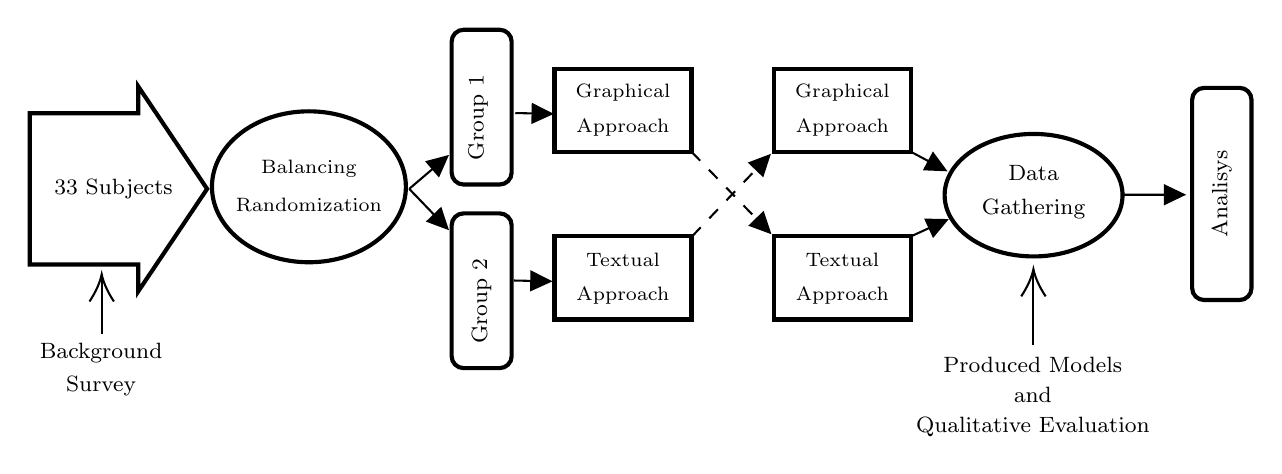
\begin{tikzpicture}[x=0.9pt,y=0.9pt,yscale=-1,xscale=1]
%uncomment if require: \path (0,327); %set diagram left start at 0, and has height of 327


%Shape: Ellipse [id:dp633810982278807] 
\draw  [line width=1.5]  (84.73,72.26) .. controls (84.73,55.52) and (102.16,41.96) .. (123.66,41.96) .. controls (145.16,41.96) and (162.59,55.52) .. (162.59,72.26) .. controls (162.59,88.99) and (145.16,102.56) .. (123.66,102.56) .. controls (102.16,102.56) and (84.73,88.99) .. (84.73,72.26) -- cycle ;



%Shape: Ellipse [id:dp7904221795411808] 
\draw  [line width=1.5]  (378.89,75.63) .. controls (378.89,62.05) and (394.88,51.04) .. (414.61,51.04) .. controls (434.33,51.04) and (450.32,62.05) .. (450.32,75.63) .. controls (450.32,89.21) and (434.33,100.22) .. (414.61,100.22) .. controls (394.88,100.22) and (378.89,89.21) .. (378.89,75.63) -- cycle ;

%Rounded Rect [id:dp5302697683495847] 
\draw  [line width=1.5]  (180.95,87.75) .. controls (180.95,85.09) and (183.11,82.93) .. (185.77,82.93) -- (200.23,82.93) .. controls (202.9,82.93) and (205.06,85.09) .. (205.06,87.75) -- (205.06,140.25) .. controls (205.06,142.91) and (202.9,145.07) .. (200.23,145.07) -- (185.77,145.07) .. controls (183.11,145.07) and (180.95,142.91) .. (180.95,140.25) -- cycle ;
%Rounded Rect [id:dp9616486966995694] 
\draw  [line width=1.5]  (180.95,14.03) .. controls (180.95,11.37) and (183.11,9.21) .. (185.77,9.21) -- (200.23,9.21) .. controls (202.9,9.21) and (205.06,11.37) .. (205.06,14.03) -- (205.06,66.52) .. controls (205.06,69.19) and (202.9,71.35) .. (200.23,71.35) -- (185.77,71.35) .. controls (183.11,71.35) and (180.95,69.19) .. (180.95,66.52) -- cycle ;

%Shape: Rectangle [id:dp03801896284105699] 
\draw  [line width=1.5]  (222.23,24.87) -- (277.28,24.87) -- (277.28,58.21) -- (222.23,58.21) -- cycle ;
%Straight Lines [id:da1799424135415575] 
\draw    (163.93,73.09) -- (177.61,61.43) ;
\draw [shift={(179.89,59.48)}, rotate = 499.54] [fill={rgb, 255:red, 0; green, 0; blue, 0 }  ][line width=0.08]  [draw opacity=0] (8.93,-4.29) -- (0,0) -- (8.93,4.29) -- cycle    ;
%Straight Lines [id:da17029537209985257] 
\draw    (163.93,73.09) -- (177.81,87.53) ;
\draw [shift={(179.89,89.69)}, rotate = 226.13] [fill={rgb, 255:red, 0; green, 0; blue, 0 }  ][line width=0.08]  [draw opacity=0] (8.93,-4.29) -- (0,0) -- (8.93,4.29) -- cycle    ;
%Straight Lines [id:da39402523544663426] 
\draw  [dash pattern={on 4.5pt off 4.5pt}]  (277.5,92.15) -- (307.06,61.21) ;
\draw [shift={(309.13,59.04)}, rotate = 493.69] [fill={rgb, 255:red, 0; green, 0; blue, 0 }  ][line width=0.08]  [draw opacity=0] (8.93,-4.29) -- (0,0) -- (8.93,4.29) -- cycle    ;
%Straight Lines [id:da7992081880522388] 
\draw  [dash pattern={on 4.5pt off 4.5pt}]  (277.28,58.21) -- (307.27,89.16) ;
\draw [shift={(309.35,91.31)}, rotate = 225.9] [fill={rgb, 255:red, 0; green, 0; blue, 0 }  ][line width=0.08]  [draw opacity=0] (8.93,-4.29) -- (0,0) -- (8.93,4.29) -- cycle    ;
%Right Arrow [id:dp3913444800583221] 
\draw  [line width=1.5]  (11.57,42.74) -- (55.14,42.74) -- (55.14,31.99) -- (82.78,73.11) -- (55.14,114.23) -- (55.14,103.49) -- (11.57,103.49) -- cycle ;
%Shape: Rectangle [id:dp003852149638719382] 
\draw  [line width=1.5]  (310.31,24.87) -- (365.36,24.87) -- (365.36,58.21) -- (310.31,58.21) -- cycle ;
%Shape: Rectangle [id:dp0126542660109914] 
\draw  [line width=1.5]  (310.31,92.18) -- (365.36,92.18) -- (365.36,125.52) -- (310.31,125.52) -- cycle ;
%Shape: Rectangle [id:dp4954877903085966] 
\draw  [line width=1.5]  (222.23,92.18) -- (277.28,92.18) -- (277.28,125.52) -- (222.23,125.52) -- cycle ;
%Straight Lines [id:da3442884963113835] 
\draw    (365.36,58.21) -- (377.4,64.63) ;
\draw [shift={(380.04,66.05)}, rotate = 208.07999999999998] [fill={rgb, 255:red, 0; green, 0; blue, 0 }  ][line width=0.08]  [draw opacity=0] (8.93,-4.29) -- (0,0) -- (8.93,4.29) -- cycle    ;
%Straight Lines [id:da6883068419855551] 
\draw    (365.36,92.18) -- (377.84,86.46) ;
\draw [shift={(380.57,85.22)}, rotate = 515.4100000000001] [fill={rgb, 255:red, 0; green, 0; blue, 0 }  ][line width=0.08]  [draw opacity=0] (8.93,-4.29) -- (0,0) -- (8.93,4.29) -- cycle    ;
%Rounded Rect [id:dp5928061300931144] 
\draw  [line width=1.5]  (478.27,37.32) .. controls (478.27,34.68) and (480.41,32.55) .. (483.04,32.55) -- (497.34,32.55) .. controls (499.97,32.55) and (502.1,34.68) .. (502.1,37.32) -- (502.1,112.96) .. controls (502.1,115.59) and (499.97,117.72) .. (497.34,117.72) -- (483.04,117.72) .. controls (480.41,117.72) and (478.27,115.59) .. (478.27,112.96) -- cycle ;

%Straight Lines [id:da6932528701926595] 
\draw    (450.32,75.46) -- (472.85,75.45) ;
\draw [shift={(475.85,75.45)}, rotate = 539.96] [fill={rgb, 255:red, 0; green, 0; blue, 0 }  ][line width=0.08]  [draw opacity=0] (8.93,-4.29) -- (0,0) -- (8.93,4.29) -- cycle    ;
%Straight Lines [id:da7950818392289087] 
\draw    (40.46,131.56) -- (40.46,109.39) ;
\draw [shift={(40.46,107.39)}, rotate = 450] [color={rgb, 255:red, 0; green, 0; blue, 0 }  ][line width=0.75]    (10.93,-4.9) .. controls (6.95,-2.3) and (3.31,-0.67) .. (0,0) .. controls (3.31,0.67) and (6.95,2.3) .. (10.93,4.9)   ;
%Straight Lines [id:da5784112946450906] 
\draw    (414.54,135.73) -- (414.54,107.33) ;
\draw [shift={(414.54,105.33)}, rotate = 450] [color={rgb, 255:red, 0; green, 0; blue, 0 }  ][line width=0.75]    (10.93,-4.9) .. controls (6.95,-2.3) and (3.31,-0.67) .. (0,0) .. controls (3.31,0.67) and (6.95,2.3) .. (10.93,4.9)   ;
%Straight Lines [id:da04489153588175898] 
\draw    (206.5,42.65) -- (218.97,42.92) ;
\draw [shift={(221.97,42.99)}, rotate = 181.23] [fill={rgb, 255:red, 0; green, 0; blue, 0 }  ][line width=0.08]  [draw opacity=0] (8.93,-4.29) -- (0,0) -- (8.93,4.29) -- cycle    ;
%Straight Lines [id:da30869554668079413] 
\draw    (205.97,109.89) -- (218.45,110.16) ;
\draw [shift={(221.44,110.22)}, rotate = 181.23] [fill={rgb, 255:red, 0; green, 0; blue, 0 }  ][line width=0.08]  [draw opacity=0] (8.93,-4.29) -- (0,0) -- (8.93,4.29) -- cycle    ;




% Text Node
\draw (249.75,48.63) node  [font=\scriptsize] [align=left] {Approach};
% Text Node
\draw (249.75,34.46) node  [font=\scriptsize] [align=left] {Graphical};
% Text Node
\draw (490.19,75.14) node  [font=\footnotesize,rotate=-270] [align=left] {Analisys};
% Text Node
\draw (414.31,168.64) node  [font=\footnotesize] [align=left] {Qualitative Evaluation};
% Text Node
\draw (414.31,155.81) node  [font=\footnotesize] [align=left] {and};
% Text Node
\draw (414.31,143.84) node  [font=\footnotesize] [align=left] {Produced Models};
% Text Node
\draw (187.85,136.5) node [anchor=north west][inner sep=0.75pt]  [font=\footnotesize,rotate=-270] [align=left] {Group 2};
% Text Node
\draw (337.84,34.46) node  [font=\scriptsize] [align=left] {Graphical};
% Text Node
\draw (337.84,48.63) node  [font=\scriptsize] [align=left] {Approach};
% Text Node
\draw (249.75,101.76) node  [font=\scriptsize] [align=left] {Textual};
% Text Node
\draw (249.75,115.93) node  [font=\scriptsize] [align=left] {Approach};
% Text Node
\draw (337.84,101.76) node  [font=\scriptsize] [align=left] {Textual};
% Text Node
\draw (337.84,115.93) node  [font=\scriptsize] [align=left] {Approach};
% Text Node
\draw (414.61,66.67) node  [font=\footnotesize] [align=left] {Data};
% Text Node
\draw (414.61,81.26) node  [font=\footnotesize] [align=left] {Gathering};
% Text Node
\draw (40.22,138.89) node  [font=\footnotesize] [align=left] {Background};
% Text Node
\draw (40.22,152.23) node  [font=\footnotesize] [align=left] {Survey};
% Text Node
\draw (123.66,64.96) node  [font=\scriptsize] [align=left] {Balancing};
% Text Node
\draw (123.66,79.56) node  [font=\scriptsize] [align=left] {Randomization};
% Text Node
\draw (186.5,62.78) node [anchor=north west][inner sep=0.75pt]  [font=\footnotesize,rotate=-270] [align=left] {Group 1};
% Text Node
\draw (45.21,73.11) node  [font=\footnotesize] [align=left] {33 Subjects};


\end{tikzpicture}

    % \includegraphics[width=\columnwidth]{images/DesignExperimento.png}
    \fonte{Author.}
\end{figure}

%###########################################################
\subsection{Conduction}
\label{ssec_experiments:preliminary_conduction}
%###########################################################

\textbf{Preparation:} 
Initially, we held remote meetings between the researchers involved to define the planning and the adopted operation mode in response to the current exception scenario due to the worldwide pandemic.
% Initially, remote meetings were held between the researchers involved to define the planning and the mode of operation that should be adopted, in response to the current scenario of exception due to the worldwide pandemic.
As a result, we defined activities adapted from the first experiment conducted in person.
% As a result, activities were defined that should be adapted in relation to the first experiment, which was conducted in person.
Hence, to capture a significant sample for the object of study, we decided to contact the professors responsible for teaching, in the first half of 2021, two courses of different undergraduate courses: Database (SE) and Database I (CS).
% In order to capture a significant sample for the object of study, it was decided to contact the professors responsible for teaching two courses of different undergraduate courses: Database (SE) and Database I (CS) in the first half of 2021.
% With the initial objectives aligned, the collaborating teachers made the disclosure of profile questionnaires (Google Forms) to the subjects.
Once the initial objectives aligned, the collaborating teachers disclosed the profile questionnaires (Google Forms) to the subjects.

We reused the four (4) instruments from the original experiment. 
% The four (4) instruments from the original experiment were reused. 
The first two were modeling problems with similar levels of complexity, while the last two were qualitative assessments.
% The first two were modeling problems with similar levels of complexity, while the last two were of qualitative assessment.
For respecting the health security protocols required (social distancing), we decided to carry out the activities remotely.
% We decided that the activities would carry out remotely, respecting the health security protocols required (social distancing). 
% It was decided that the activities would be carried out remotely, respecting the health security protocols required (social distancing). 
For this purpose, we prepared a virtual machine with the tools installed, even as the instruments and supporting materials. 
% For this purpose, a virtual machine was prepared with the tools installed, as well as the instruments and supporting materials. 
This virtual machine had accessed on the university's computers by the subjects using their institutional credentials.
% This virtual machine should be accessed on the university's computers by the subjects using their institutional credentials.

\textbf{Execution:} 
The profile form also served as a term of participation since the presence in the experiment was voluntary.
With this information, we have randomized the subjects to define the groups.
% With this information, the subjects were then randomized to define the groups.
We did not find wide discrepancies among the subjects' knowledge levels, demonstrating a homogeneous sample in general.
% We found that there were no major discrepancies between the levels of knowledge of the subjects, demonstrating that there was a homogeneous sample in general.
On the experiment day, the first activity that we performed was a brief initial presentation.
% On the experiment day, the first activity carried out was a brief initial presentation.
Then, the training phase for the participants began.
During this phase, we have presented the two database modeling tools used in the experiment, providing an overview of the operation and answering possible questions that arose.
% During this phase, the two database modeling tools that would be used were presented, providing an overview of the operation and answering possible questions that arose.
The training phase included watching videos to demonstrate both tools: brModelo, and our proposal, respectively.

Then, we start the modeling phase of the proposed problems.
All subjects accessed the virtual machines with the problems provided in PDF documents.
% When starting Instrument 1, all participants were informed with which tool they should develop the solution, thus respecting the groups to which they were part.
When starting Instrument 1, we informed which tool each participant should develop the solution, thus respecting the group of which one was part.
We asked the subjects to write down the start and end times of the tasks for each instrument they performed.
We stipulated no time limit for completion according to the subjects who completed the modeling task. 
We asked them to comply with the guidelines included in the support material for saving the generated artifacts.
% We stipulated no time limit for completion and, according to the subjects completed the modeling task, they were asked to comply with the guidelines included in the support material for saving the generated artifacts.
With the models saved, we informed the subjects that they should move on to the next task described in Instrument 2, although it was necessary to use the reverse approach to the one they had initially used.

Since the subjects concluded the instruments of the data modeling problems, we delivered the qualitative assessment instruments.
% At the end of the instruments that contained the modeling problems, we delivered the qualitative assessment instruments.
As the subjects had completed the tasks, we had thanked and released them.
With the conclusion of the experiment by 33 subjects, we closed the evaluation and performed the stage of result analysis.

%###########################################################
\subsection{Results Analysis}
\label{ssec_experiments:preliminary_resultAnalysis}
%###########################################################

We have performed all Kolmogorov-Smirnov and Wilcoxon Signed-Rank calculations with the support of the R language and the Gnumeric software. In parallel with the validation of a specialist in the statistics field and the aid of literature~\cite{Triola:2018}.
% All Kolmogorov-Smirnov and Wilcoxon Signed-Rank calculations were performed with the support of the R language and the Gnumeric software, in parallel with the validation of a specialist in the field of statistics and the aid of literature~\cite{Triola:2018}.

\textbf{Effort:} 
To answer \textbf{RQ1.},  
%regarding the effort to use the approaches, 
% the execution times were extracted from the instruments.
we have extracted the execution times from the instruments.
From the gross amount of the execution times, we have calculated the difference to perform the Kolmogorov-Smirnov normality test.
Because it is a statistical test, this technique has the product of measuring the $p$-value.
For this test, we adopted a significance level of $\alpha$~=~5\%.
It means that the p-value is less than 5\%, then we rejected the hypothesis that the distribution is normal.
% This means that the $p$-value is less than 5\% ($p$ < 0.05), a hypothesis that the distribution is normal should be rejected.

After calculations with the set of time differences, we reached a $p$-value of 0.26218.
As $p$-value > $\alpha$, we do not reject the null hypothesis, thus concluding that the data are normally distributed.
%\textit{i.e.}, 
In other words, the difference between the data sample and the normal distribution is not large enough to be statistically significant.
It is important to note that the higher the $p$-value, the more it supports a null hypothesis.
% In the case of the result obtained, the chance of type 1 error (rejecting a null hypothesis that is correct) is very high, and can be translated into 26.21\% (0.26218).
In the case of the result obtained, the chance of type 1 error (rejecting a correct null hypothesis) is very high and translates into 26.21\% (0.26218).
Once we performed the normality tests on the sample, we carried out the hypothesis test of the average effort regarding \textbf{RQ1.}
In the Wilcoxon Signed-Rank test for dependent samples, we used a significance level of $\alpha$~=~5\%, with which we reached a measure of 0.77948 for the $p$-value.
Because it is a two-tailed test, \textit{i.e.}, it includes equality in its null hypothesis, this $p$-value shows not enough evidence to guarantee the rejection of the statement of $H_0: \mu Time_G = \mu Time_T$.
Therefore, we do not reject the null hypothesis that the approaches have no difference in average efforts since, according to the test, this difference is not statistically significant. 
Figure \ref{fig:boxplotTempo1} displays a box plot with the variation of data observed through these data.

% \begin{figure}[!htb]
%     \centering
%     % \includegraphics[width=.9\columnwidth]{experimentResults/EsforcoBoxplot.pdf}
%     % \begin{tikzpicture}
%   \begin{axis}
%     [
    % boxplot/draw direction=y,
    % xtick={1, 2},
    % ylabel={\footnotesize Time (minutes)},
    % xticklabels={{\footnotesize Graphical Treatment}, {\footnotesize Textual Treatment}},
    % height= 5cm
%     ]
%     \addplot+[fill=olive, fill opacity=0.7, draw=black,
%     boxplot prepared={
%       median=25.00,
%       upper quartile=28.00,
%       lower quartile=21.00,
%       upper whisker=60.00,
%       lower whisker=12.00
%     },
%     ] coordinates {};
%     \addplot+[fill=teal, fill opacity=0.7, draw=black,
%     boxplot prepared={
%       median=33.00,
%       upper quartile=43.00,
%       lower quartile=27.00,
%       upper whisker=60.00,
%       lower whisker=15.00
%     },
%     ] coordinates {};
%   \end{axis}
% \end{tikzpicture}

\begin{filecontents*}{data.csv}
11,12,14,15,17,17,19,19,20,21,30,30,32,32,32,33,35,35,35,37,39,42,43,45,45,46,48,50,51,51,51,60,60
17,20,21,21,23,23,24,26,26,26,27,27,30,31,31,34,36,38,38,38,39,40,40,40,40,44,46,47,48,49,50,52,60
\end{filecontents*}

\begin{tikzpicture}
    \pgfplotstableread[col sep=comma]{data.csv}\csvdata
    % Boxplot groups columns, but we want rows
    \pgfplotstabletranspose\datatransposed{\csvdata} 
    \begin{axis}[
        boxplot/draw direction=y,
        xtick={1, 2},
        ylabel={\scriptsize Time (minutes)},
        xticklabels={{\scriptsize Graphical Treatment}, {\scriptsize Textual Treatment}},
        height=7cm,
        width=10cm,
        % boxplot/draw direction = y,
        % axis x line* = bottom,
        % axis y line = left,
        % enlarge y limits,
        ymajorgrids,
        % xtick = {1, 2},
        % xticklabel style = {align=center, font=\small},
        % xticklabels = {Graphical Treatment, Textual Treatment},
        % ylabel = {Time (minutes)},
        ytick = {15, 30, 45, 60},
        yticklabel style = {font=\scriptsize}
    ]
        \foreach \n in {1,...,2} {
            \addplot+[boxplot, fill, fill opacity=0.4, draw=black] table[y index=\n] {\datatransposed};
        }
    \end{axis}
\end{tikzpicture}


%     % \includesvg[width=.7\columnwidth]{figures/Effort}
%     \caption{Box-plot - Effort per treatments.}
%     \label{fig:boxplotTempo1}
% \end{figure}

\textbf{Effectiveness:} 
% To answer \textbf{RQ2.} regarding the effectiveness of the use of approaches
To answer \textbf{RQ2.}, regarding the approaches' use effectiveness, we evaluated the artifacts produced by the subjects according to the established reference models\footnote{Available at: \url{https://doi.org/10.5281/zenodo.5454378}}. 
In this evaluation, we used the F1 applied to the pattern recognition and the information retrieval areas.
% In this evaluation, we used F1 from the area of pattern recognition and information retrieval. 
F1 represents the combination of the observed accuracy and the recallability of a result concerning a reference.
By definition, this combination refers to Precision and Recall metrics. On the one hand, Precision is the ratio of the recovered instances by relevance. On the other hand, Recall is the ratio of the relevant instances to the recovered.
% By definition, this combination refers to Precision and Recall metrics, where Precision is the proportion of recovered instances that are relevant and Recall is the proportion of relevant instances that are recovered.

In addition, we performed the Kolmogorov-Smirnov normality test to F1 for each model. 
After calculations with the set of differences in F1 for each model, we reached a $p$-value of 0.45459.
With this test result, the chance of type 1 error (rejecting a correct null hypothesis) can be very high, and hence we can translate it into 45.45\% (0.45459).
%With this test result, the chance of type 1 error (rejecting a correct null hypothesis) can be very high, and can be translated into 45.45\% (0.45459).
As the $p$-value > $\alpha$, we do not reject the null hypothesis, thus realizing that the data are a normal distribution.
%As the $p$-value > $\alpha$, we do not reject the null hypothesis, thus realizing that the data is normally distributed.
%, \textit{i.e.} the difference between the data sample and the normal distribution is not large enough to be statistically significant.
After we tested the sample for normality, we tested the second hypothesis defined in this experiment.
%After the sample was tested for normality, we tested the second hypothesis defined in this experiment.
This time, in the Wilcoxon Signed-Rank test for dependent samples, we used again a significance level of $\alpha$~=~5\%, with which we reached a measure of 0.00197 for the $p$-value.
% By the original statement including an equality, also characterizing this test as two-tailed, it was concluded that the calculated $p$-value demonstrates that there is enough evidence to guarantee the rejection of the statement of the original null hypothesis, denoted as $H_0: \mu Effectiveness_G = \mu Effectiveness_T$.
By the original statement including equality, also characterizing this test as two-tailed, we concluded that the calculated $p$-value demonstrated enough evidence to guarantee the statement rejection of the primary null hypothesis, denoted as $H_0: \mu Effectiveness_G = \mu Effectiveness_T$.
% Therefore, we reject the null hypothesis that the approaches have equal effectiveness, because according to the statistical test, the average difference of F1 among treatments is statistically significant.
Therefore, we rejected the null hypothesis that the approaches have equal effectiveness since, according to the statistical test, the average difference of F1 among treatments is statistically significant.
Table \ref{tab:ResultsModelosGeral} shows average measures of the evaluated values and also provides the possibility to carry out a dispersion analysis.
Based on these data, it was possible to verify that the textual approach has an advantage on average.

\rowcolors{1}{gray!15}{white}
\begin{table}[!htb]
    \caption{Measures of the conceptual data models produced in the experiment.}
    \label{tab:ResultsModelosGeral}
    \centering
    % \scriptsize
    \tiny
    \begin{tabular}{l|ccccc|ccccc}%{l|ccccc|ccccc}
    \bottomrule
    \rowcolor[HTML]{C0C0C0}
    \multicolumn{1}{l}{} &
    \multicolumn{5}{c|}{\textbf{Graphical Treatment}} &
    \multicolumn{5}{c}{\textbf{Textual Treatment}}
    \\ 
    \hline
    \rowcolor[HTML]{C0C0C0}
    \textbf{Measure} & \textbf{MI} & \textbf{RI} & \textbf{P(\%)} & \textbf{R(\%)} & \textbf{F1(\%)} &
    \textbf{MI} & \textbf{RI} & \textbf{P(\%)} & \textbf{R(\%)} & \textbf{F1(\%)}
    \\
    \hline
Maximum	&	47.00	&	36.00	&	96.67	&	92.31	&	88.00	&	56.00	&	46.00	&	97.22	&	97.87	&	91.36	\\
3\textdegree Quartile	&	31.00	&	28.00	&	92.31	&	63.04	&	76.32	&	34.00	&	31.00	&	94.74	&	75.00	&	82.86	\\
Median	&	26.00	&	24.00	&	88.89	&	56.41	&	68.85	&	30.00	&	29.00	&	90.63	&	65.96	&	74.63	\\
Average	&	27.52	&	24.12	&	87.69	&	57.96	&	69.13	&	30.88	&	27.45	&	89.49	&	63.65	&	73.16	\\
1\textdegree Quartile	&	23.00	&	20.00	&	84.21	&	50.00	&	62.50	&	26.00	&	23.00	&	87.88	&	51.06	&	63.01	\\
Minimum	&	18.00	&	16.00	&	72.73	&	41.03	&	52.46	&	19.00	&	15.00	&	72.73	&	31.91	&	45.45	\\
Variance	&	35.58	&	28.65	&	42.87	&	143.35	&	78.93	&	63.32	&	39.76	&	42.59	&	259.85	&	133.58	\\
SD &	5.97	&	5.35	&	6.55	&	11.97	&	8.88	&	7.96	&	6.31	&	6.53	&	16.12	&	11.56	\\
    \toprule
\end{tabular}
\begin{tablenotes}
    \scriptsize
    \centering
    \item \textit{Legend: MI = Modeled Items; RI = Relevant Items; P = Precision; R = Recall; F1 = F1-Score; SD = Standard Deviation.}
\end{tablenotes}
\fonte{Author.}
\end{table}

Figure \ref{fig:boxplotMedidaF1} box plot graph displays the F1-Score for each treatment applied. 
Based on this graph, it is possible to verify the result obtained in the hypothesis test because the data dispersion does present a significant difference between the approaches.

\begin{figure}[!htb]
        \centering
        \caption{Box-plot - Effort per treatments.}
        \label{fig:boxplotTempo1}
        \include{img/BoxPlotEsforco1}
        \fonte{Author.}
\end{figure}

\begin{figure}[!htb]
        \centering
        \caption{Box-plot - F1 per treatments.}
        \label{fig:boxplotMedidaF1}
        \include{img/boxplotMedidaF1}
        \fonte{Author.}
\end{figure}

% \begin{figure}[!htb]
%     \centering
%     % \includegraphics[width=.9\columnwidth]{experimentResults/EfetividadeBoxplot.pdf}
%     \include{figures/boxplotMedidaF1}
%     % \includesvg[width=.7\columnwidth]{figures/F-Score}
%     \caption{Box-plot - F1 per treatments.}
%     \label{fig:boxplotMedidaF1}
% \end{figure}

\textbf{Qualitative Evaluation:} 
We took place with the analysis of the two instruments applied after the modeling tasks.
We have used the first instrument according to the TAM model~\cite{Davis:1989,Persico:2014} to answer the \textbf{RQ3.} regarding the PEoU and PU.
% The first was used to respond to \textbf{RQ3.} regarding the PEoU and PU of treatments, according to the TAM model~\cite{Davis:1989,Persico:2014}. 
It occurred through the quality attributes selection described in ISO/IEC 25010.
For this to happen, we established a Likert~\cite{Likert} scale from one to six points to measure the subjects' agreement level in the face of the statements exposed in the form.
% For this, we established a Likert scale from one to six points to measure the level of agreement of the subjects in the face of the statements exposed in the form.
We have chosen an even number of alternatives to avoid possible neutral responses.
% This scale served to measure the level of agreement of the subjects in the face of the statements exposed in the form.
Thus, we grouped the seven (7) quality attributes into three (3) defined categories as follows:
% Thus, the 7 quality attributes are grouped into three (3) categories being defined as follows:

\begin{itemize}
% \begin{inparaenum}
    \item \textbf{Functionality} 
        \begin{itemize}
            \item \textit{Conformity}: ability level to which the software achieves specified goals with functional completeness, correctness, and appropriateness related to their functionalities.
        \end{itemize}
    \item \textbf{Usability}
        \begin{itemize}
            %Appropriateness recognisability
            \item \textit{Understandability}: ability level to which users can recognize whether the software is appropriate for their needs; 
            \item \textit{Learnability}: ability level to which the software enables the user to learn how to use it with effectiveness, efficiency in emergencies;
            \item \textit{Operability}: ability level to which the software is easy to operate and control, being also appropriate to use.
            %\item \textit{Operability}: ability level to which the software is easy to operate, control, and appropriate to use.
        \end{itemize}
    \item \textbf{Quality in Use}
        \begin{itemize}
            \item \textit{Quality in Use}: ability level to which the software achieves specified goals with effectiveness and efficiency with their users when used in specified contexts;
            % Performance Efficiency
            \item \textit{Productivity}: ability level to which the software to achieve specified goals with time-behavior, resources utilization, and capacity when performing its functions to meet requirements;
            \item \textit{Satisfaction}: ability level to which the software achieves specified goals with usefulness, trust, pleasure, and comfort with their users when used in specified contexts.
        \end{itemize}
        % \end{inparadesc}
% \end{inparaenum}
\end{itemize}

After summarizing the results, we observed a good acceptance by the subjects for the ERtext tool developed in this work.
Figure \ref{fig:inst3GERALExp} synthesizes the responses received for each quality attribute, showing a certain degree of similarity in the subjects' perception during the application of the treatments.
% A point that can be emphasized is the set of positive responses concerning the \textit{Productivity} and \textit{Operability} since in the hypothesis test related to the effort, the treatments demonstrated a similar need for execution time.
It is worth emphasizing a point that is the positive responses set concerning the \textit{Productivity} and \textit{Operability} since the hypothesis test related to the effort the treatments demonstrated a similar need for execution time.
According to the evaluations received, the most evidence about disadvantages of ERtext was mainly concerning the quality attributes of \textit{Understandability} and \textit{Learnability}.
%According to the evaluations received, the most evident disadvantages of ERtext are manifested mainly concerning \textit{Understandability} and \textit{Learnability} quality attributes.

\begin{figure}[!htb]
    \centering
    \caption{Quality attributes per treatments.}
    \label{fig:inst3GERALExp}
    % \includegraphics[width=.9\columnwidth]{experimentResults/Inst3.png}
    \pgfplotsset{testbar/.style={
        xbar stacked,
        legend cell align=left,
        legend style={
            legend columns=8,
            font=\scriptsize,
            at={(xticklabel cs:1.0)},
            anchor=north east,
            draw=none,
            nodes={scale=1}
            },
        width=10cm,
        axis y line*= none, 
        axis x line*= bottom,
        xmajorgrids = false,
        xmin=0,xmax=33,
        ytick = data,
        yticklabels = {
            {\scriptsize Conformity-ERtext},
            {\scriptsize Conformity-brModelo},
            {\scriptsize Understandability-ERtext}, %Intelligibility
            {\scriptsize Understandability-brModelo},
            {\scriptsize Learnability-ERtext}, %Apprehensibility
            {\scriptsize Learnability-brModelo}, 
            {\scriptsize Operability-ERtext},
            {\scriptsize Operability-brModelo},
            {\scriptsize Quality in Use-ERtext},
            {\scriptsize Quality in Use-brModelo},
            {\scriptsize Productivity-ERtext}, %Performance Efficiency
            {\scriptsize Productivity-brModelo},
            {\scriptsize Satisfaction-ERtext},
            {\scriptsize Satisfaction-brModelo}
        },
        tick align = outside, 
        xtick pos = left,
        xticklabel style = {font=\scriptsize},
        bar width=3.5mm, 
        y=6.5mm,
        enlarge y limits={abs=0.450},% 0.5 + 0.5*(y - bar width)/y [TeX.sx #47995]
        nodes near coords,
        nodes near coords align=center,%Move values in bar
        every node near coord/.append style={
            black,
            font=\scriptsize,
            text opacity=1,
            fill=white,
            fill opacity=0.5,
            outer sep=\pgflinewidth
        }
    }}
    \begin{tikzpicture}
    \begin{axis}[testbar] 
    \addplot[pattern color=red,pattern=north east lines] coordinates
        {(0,14)(1,13)(1,12)(1,11)(2,10)(1,9)(1,8)(1,7)(0,6)(1,5)(2,4)(2,3)(0,2)(1,1)};
    \addplot[pattern color=teal,pattern=vertical lines] coordinates
        {(2,14)(0,13)(0,12)(0,11)(0,10)(0,9)(0,8)(1,7)(0,6)(0,5)(0,4)(0,3)(2,2)(2,1)};
    \addplot[pattern color=gray, pattern=grid] coordinates
       {(0,14)(1,13)(2,12)(0,11)(3,10)(1,9)(0,8)(3,7)(2,6)(2,5)(1,4)(5,3)(1,2)(1,1)};
    \addplot[pattern color=magenta, pattern=north west lines] coordinates
       {(4,14)(2,13)(3,12)(1,11)(10,10)(5,9)(7,8)(9,7)(2,6)(2,5)(7,4)(4,3)(4,2)(6,1)};
    \addplot[pattern color=blue, pattern=horizontal lines] coordinates
       {(11,14)(11,13)(10,12)(7,11)(11,10)(11,9)(12,8)(9,7)(11,6)(10,5)(11,4)(13,3)(10,2)(9,1)};
    \addplot[pattern color=green, pattern=crosshatch dots] coordinates
       {(16,14)(18,13)(17,12)(24,11)(7,10)(15,9)(13,8)(10,7)(18,6)(18,5)(12,4)(9,3)(16,2)(14,1)};
    \legend{1-Disagree, 2, 3, 4, 5, 6-Agree}
    \end{axis}
    \end{tikzpicture}
    
% \begin{tikzpicture}
% \begin{axis}[
%     xbar stacked,
%     legend cell align=center,
%     legend style={
%     legend columns=5,
%         at={(xticklabel cs:1.0)},
%         anchor=north east,
%         draw=none
%     },
%     ytick=data,
%     axis y line*=none,
%     axis x line*=bottom,
%     tick label style={font=\small},
%     legend style={font=\small},
%     label style={font=\small},
%     xtick={0,3,6},
%     xticklabel= {},
%     bar width=5mm,
%     ylabel={Questions},
%     yticklabels={P-Q1, T-Q1, P-Q2, T-Q2, P-Q3, T-Q3, P-Q4, T-Q4,P-Q5, T-Q5,P-Q6, T-Q6, P-Q7, T-Q7},
%     xmin=0,
%     xmax=6,
%     area legend,
%     y=6.5mm,
%     enlarge y limits={abs=0.625},
%     nodes near coords,
%     nodes near coords align=center,
%     every node near coord/.append style={
%         black,
%         font=\small,
%         text opacity=.65,
%         fill=white,
%         fill opacity=0.75,
%         outer sep=\pgflinewidth
%     }
% ]
% \addplot[pattern color=red,pattern=horizontal lines] coordinates
% {(0,14)(0,13)(0,12)(0,11) (3,10)(0,9)(0,8) (0,7) (0,6)(0,5)(0,4) (0,3) (0,2) (0,1)};   
% \addplot[pattern color=orange,pattern=grid] coordinates
% {(3,14) (0,13)(0,12)(0,11)(2,10) (1,9)(1,8)(0,7)(3,6)(0,5)(0,4)(3,3) (4,2) (0,1) };  
% \addplot[pattern color = green, pattern=crosshatch dots] coordinates
% {(0,14) (0,13) (3,12)(2,11)(1,10) (3,9)(4,8)(1,7)(3,6)(1,5)(3,4)(2,3)(2,2) (2,1) };   
% \addplot[pattern color=blue, pattern =vertical lines ] coordinates
% {(2,14) (3,13) (2,12)(3,11)(0,10)(2,9)(1,8)(4,7)(0,6)(3,5) (3,4)(1,3)(0,2)(4,1)};   
% \addplot[pattern color=gray, pattern = dots] coordinates
% {(1,14)(3,13)(1,12)(1,11)(0,10)(0,9)(0,8)(1,7) (0,6)(2,5) (0,4)(0,3)(0,2)(0,1) };   
% \legend{1-Disagree, 2, 3, 4, 5-Agree}

% \end{axis}
% \end{tikzpicture}
% \footnotesize
% T-Thoth answers; P-Parsifal answers;






% \begin{tikzpicture}
% \begin{axis}[
%     xbar stacked,
%     legend cell align=left,
%     legend style={
%     legend columns=2,
%         at={(xticklabel cs:1.0)},
%         anchor=north east,
%         draw=none
%     },
%     ytick=data,
%     axis y line*=none,
%     axis x line*=bottom,
%     tick label style={font=\scriptsize},
%     legend style={font=\scriptsize},
%     %legend style={font=\scriptsize,row sep=-0.1cm,/tikz/every odd column/.append style={column sep=0.01cm}},
%     label style={font=\scriptsize},
%     xtick={0,10,...,100},
%     width=\columnwidth,
%     bar width=3.5mm,
%     % xlabel={Frequencia em \%},
%     yticklabels={
%     {Q1 - OC},
%     {Q2 - TD},
%     {Q3 - OC},
%     {Q4 - TD},
%     {Q5 - OC},
%     {Q6 - TD},
%     {Q7 - OC},
%     {Q8 - TD},
%     {Q9 - OC},
%     {Q10 - TD},
%     {Q11 - OC},
%     {Q12 - TD}},
%     xmin=0,
%     xmax=100,
%     area legend,
%     y=5mm,
%     enlarge y limits={abs=0.625},
%     nodes near coords,
%     nodes near coords={\pgfmathprintnumber\pgfplotspointmeta\%},
%     nodes near coords align=center,%Move values in bar
%     every node near coord/.append style={
%         black,
%         font=\footnotesize,
%         text opacity=1,
%         fill=white,
%         fill opacity=0.7,
%         outer sep=\pgflinewidth
%     }
% ]
% \addplot[pattern color=blue,pattern=dots] coordinates
% {(0,0)(0,1)(0,2)(0,3)(0,4)(0,5)(0,6)(0,7)(0,8)(0,9)(0,10)(0,11)};
% \addplot[pattern color=red, pattern=vertical lines] coordinates
% {(4,0)(32,1)(0,2)(9,3)(13,4)(18,5)(0,6)(9,7)(5,8)(5,9)(0,10)(14,11)};
% \addplot[pattern color=cyan, pattern=grid] coordinates
% {(27,0)(9,1)(4,2)(5,3)(23,4)(27,5)(36,6)(23,7)(27,8)(41,9)(46,10)(45,11)};
% \addplot[pattern color=green, pattern=horizontal lines] coordinates
% {(55,0)(32,1)(55,2)(68,3)(41,4)(50,5)(46,6)(64,7)(64,8)(45,9)(36,10)(27,11)};
% \addplot[pattern color=orange, pattern=crosshatch dots] coordinates
% {(14,0)(27,1)(41,2)(18,3)(23,4)(5,5)(18,6)(4,7)(4,8)(9,9)(18,10)(14,11)};
% \legend{Strongly disagree,Disagree,Neither agree nor disagree,Agree,Strongly agree}; 

% \end{axis}  
% \end{tikzpicture}d
    \fonte{Author.}
\end{figure}

Concerning \textbf{RQ4.} on the assessment of DSL designers, we analyzed the artifacts of the 2nd qualitative assessment instrument.
This instrument listed the 8 ER modeling builders covered by DSL, arranged with a Likert~\cite{Likert} scale from one to six points.
% Again, an even number was chosen on the scale to avoid neutral responses that could lead to a more subjective bias.
Again, we have chosen an even number on the scale to avoid neutral responses that could lead to a more subjective bias.
Figure \ref{fig:inst4GERALExp} compiles all the responses received. 
The builders related to Entities, Referential Attributes, Descriptive Attributes, and Cardinality were the best evaluated.
In contrast, all builders obtained at least one disagreement, in which we can highlight the most disagreeing evaluations related to the current representations of ternary relationship and self-relationship, unfortunately.
%In contrast, all builders obtained at least one disagreement, highlighting the most disagreeing evaluations related with the current representations of Ternary Relationship and Self-relationship, unfortunately.

\begin{figure}[!htb]
    \centering
    \caption{Evaluation of DSL designers.}
    \label{fig:inst4GERALExp}
    % \includegraphics[width=0.9\columnwidth]{experimentResults/Inst4.png}
    \include{img/Inst4}
    \fonte{Author.}
\end{figure}

All data collected and used for statistical tests can be accessed in a public repository available on the Zenodo\footnote{Available at: \url{https://doi.org/10.5281/zenodo.5454378}} platform.

%#######################################################
%#######################################################
\subsection{Threats to Validity}
\label{ssec_experiments:preliminary_threats}
%#######################################################
%#######################################################

In empirical studies, it is necessary to analyze and discuss the threats to validity also the strategies used to mitigate them.
For this list of possible threats, we adopted the classification schema proposed by Cook and Campbell~\cite{Cook:1979}.
%For the list of possible threats, we adopted the classification scheme published by Cook and Campbell~\cite{Cook:1979}. 
These threats followed the proposed pattern, and we divided them into four (4) categories: construct validity, internal validity, external validity, and conclusion validity.
% These threats followed the proposed pattern and were divided into four (4) categories, namely: construct validity, internal validity, external validity and conclusion validity.

\textbf{Construct Validity}: 
Threats to construct validity concerns the experiment design and social factors.
\begin{enumerate}[label=\roman*.]
    \item \textit{Inappropriate Pre-operational Explanation}: is related to the fact that the experiment did not have the objective of the artifacts sufficiently defined before translation into measures or treatments. To mitigate this threat, we compared the effort of each approach as well as their effectiveness carried out according to the Precision and Recall metrics; 
    %\item The fact that the experiment did not have the objective of the artifacts sufficiently defined before translation into measures or treatments becomes a threat. To mitigate this threat, we compared the effort of each approach as well as their effectiveness carried out according to the Precision and Recall metrics; 
   
    \item \textit{Interaction of Different Treatments}: 
    if the subjects are involved in one more study, the controls of the different studies can change and reverberate in the final results.
    To avoid this, we followed a paired design and, therefore, all subjects performed both treatments.
    However, we have not observed learning issues during the execution of activities.
    %However, learning issues during the execution of activities were not observed.
    We can verify this through the normality of the analyzed distributions of both samples: effort and effectiveness, demonstrating that the results remained similar as a whole with a low variation; 
    %\textit{i.e.} low standard deviation indicates that the data points tend to be very close to the mean. 
    
    % \item If the subjects are involved in one more study, the controls of the different studies, can change and reverberate in the final results. 
    % To avoid this, we followed a paired design, and therefore, all subjects performed both treatments. 
    % However, we do not observe learning issues among the execution of activities. 
    % This can be verified through the normality of the analyzed distributions of both samples: effort and effectiveness, demonstrating that the results remained similar as a whole with a low variation.
    
    \item \textit{Hypothesis Prediction}: 
    when subjects participate in an experiment, they may try to find out what the objective or intended experiment result is. 
    This threat can bias the behavior, positively or negatively, depending on the anticipated hypothesis.
    To mitigate this threat, we do not inform the subjects about further details of the experiment; 
    
    \item We do not inform the subjects about further details of the experiment to mitigate the bias of the behavior, which can affect positively or negatively, depending on the anticipated hypothesis.
\end{enumerate}

\textbf{Internal Validity}: 
Threats to internal validity are the influences that can affect independent variables in correlation to causality without the researcher's knowledge.
\begin{enumerate} [label=\roman*.]
    \item \textit{History}: there is a risk when a specific period influences the experiment's performance. Due to the coronavirus pandemic, we conducted the entire evaluation in a controlled environment providing remote access for the subjects. 
    In addition, to soothe this threat, we carried out the entire process in March when, in general, students are not necessarily overwhelmed with academic activities;
    %\item There is a risk when a specific period influences the experiment's performance. Due to the coronavirus pandemic, we conducted the entire evaluation in a controlled environment providing remote access for the subjects.
    
    \item \textit{Maturation}: occurs concerning the subjects react in different ways over time. 
    Examples are when subjects are affected negatively (tiredness or boredom) or positively (learning) during the experiment execution.
    To alleviate this threat, we informed subjects from the beginning that they could terminate their participation at any time, without any penalty;
    %\item Sometimes the subjects could be affected negatively (tiredness or boredom) or positively (learning) during the experiment execution.
    %To alleviate this threat, we informed subjects from the beginning that they could terminate their participation at any time, without any penalty;
    
    \item \textit{Tests}: 
    if we have repeated the tests, the subjects can respond differently at other times, \textit{i.e.}, they know how to perform the test. 
    If there is a need to become familiar with the tests, we do not return the test results to the participant to not subsidize intentional learning. 
    %If the tests are repeated, the subjects may respond differently at different times, as they know how the test is performed. 
    There was no need for repetition of activities since they were performed once per participant in each treatment;
    %If there is a need to familiarize yourself with the tests, the test results must not be returned to the subject, so as not to support unintentional learning. 
    
    \item \textit{Instrumentation}: 
    is related to the artifacts used to carry out the experiment study, such as data collection forms. 
    %is related to the artifacts used to perform experiment, such as data collection forms. 
    If the design of instruments is poor, then it negatively affects the experience.
    %If these are poorly designed, the experience is negatively affected.
    To combat this threat, we minimally adapted all artifacts due to the design of the experiment (remote) and previously verified and validated in meetings between the researchers involved in this work.
    %To combat this threat, all artifacts were minimally adapted due to the design of the experiment (remote), and previously verified and validated in meetings between the researchers involved in this work.
    In addition, we already had the first study with results counting 27 participants to validate the planned protocol for this experiment replication;
    
    \item We adapted all artifacts due to the design of the experiment (remote), which we verified and validated previously in meetings among the researchers involved in this work to avoid the instrumentation of artifacts that can affect the execution.
    %All artifacts were minimally adapted due to the design of the experiment (remote), and previously verified and validated in meetings between the researchers involved in this work to avoid that the instrumentation of artifacts can be affect the execution.
    In addition, we already had the first study with results counting 27 participants to validate the planned protocol for this experiment replication.
\end{enumerate}

\textbf{External Validity}: 
% Threats to external validity are conditions related to experiment replication.
\begin{enumerate}[label=\roman*.]
    % \item \textit{Experiment Subjects}: the subjects selected for the experiment may not include a significant group for an study area.
    % Seeking to mitigate this threat, the experiment was carried out with undergrad students of SE and CS programs, and soon, inserted in the context of using the conceptual modeling of relational databases. 
    % In addition, the fact that the sample has more than 30 subjects is also a way of mitigating greater statistical threats in the analyzed area.
    \item We carried out the experimental study with undergrad students of SE and CS programs and soon inserted in the context of using the conceptual database modeling seeking to mitigate the selection of subjects from a significant group for a study area; 
    %In addition, the fact that the sample has more than 30 subjects is also a way of mitigating greater statistical threats in the analyzed area.
    %\item \textit{Subjects Interaction with the Evaluation Artifacts}: is related to the application of the evaluation artifacts of the experiment with the subjects.
    %Depending on the moment, this can affect the experimental results.
    %For example, if a questionnaire is answered a few days after the execution experiment, people tend to respond differently than they would do moments after the activities.
    %To mitigate this threat, participants were asked to answer the questionnaires and, before thanking them, we checked the submission of the instruments.
    \item We asked the participants to answer the questionnaires post-experiment and, before thanking them, we checked the submission of the instruments to avoid the subjects' interaction with the evaluation artifacts can be affected the preliminary experimental results; 
    % \item \textit{Configuration and Treatment Interaction}: is related to the use of an unrepresentative configuration or material. 
    % To soften this threat, documentation was used based on templates and traditional models found in database teaching material. 
    % In addition, the artifacts were validated with two specialists in the field of SE.
    \item We used the documentation based on templates and traditional models found in database teaching material to soften an unrepresentative configuration and material.
\end{enumerate}

\textbf{Conclusion Validity}: 
% Threats to the validity of the conclusion are related to questions that affect the ability to infer a correct conclusion about the relationship between treatments and the result of an experiment.
\begin{enumerate} [label=\roman*.]
    % \item \textit{Low Statistical Power}:
    % To try mitigating this threat, some statistical methods were adopted, such as the Kolmogorov-Smirnov normality test, the Wilcoxon Signed-Rank Test as a hypothesis test for dependent samples. 
    % In addition, the tests were reviewed by an expert in the statistics field.
    \item We adopted some statistical methods such as the Kolmogorov-Smirnov normality test and the Wilcoxon Signed-Rank Test as a hypothesis test for dependent samples. We use them to try to mitigate the low statistical power of our preliminary experimental results;
    % \item \textit{Reliability of Measurements}:
    % The reliability of the measurements used has a direct impact on the validity of the experiment as a whole. 
    % To mitigate this threat, it was adopted objective measurements that did not depend on subjective judgment (effort spent, measured in time, and F1).
    % On the other hand, the metrics used for the qualitative evaluation still served as a complementary input in the discussion of the results obtained, alongside with the indication of possible points of improvement in our proposal.
    \item We adopted objective measurements that did not depend on subjective judgment (effort spent, measured in time, and F1) to mitigate the measurement reliability threat.
    On the other hand, the metrics used for the qualitative evaluation still served as a complementary input in the results obtained discussion, alongside the indication of possible points of improvement in our proposal;
    % \textit{Experimental Environment}:
    % The experiment must be carried out in a controlled environment.
    % In order to mitigate this possible threat, we created copies of a virtual machine that were accessed by all subjects. 
    % We also instructed subjects that conversations could not take place during the entire execution of activities, in addition to not leaving the remote environment or access other electronic devices before the end of the tasks.
    \item We created copies of a virtual machine that all subjects accessed to guarantee that we experimented in a controlled environment.
    %We created copies of a virtual machine that were accessed by all subjects to guarantee that the experiment was carried out in a controlled environment.
    %Also, we instructed subjects that conversations could not take place during the entire execution of activities, in addition to not leaving the remote environment or access other electronic devices before the end of the tasks.
\end{enumerate}

%------------------------------------------------------------------------------
\section{Learning and Tool Features - Experiment 2 and 3}
\label{sec_experiments:finalEval}
%------------------------------------------------------------------------------

% A meta das avaliações experimentais finais foi realizar dinâmicas similares com a descrita na Seção \ref{sec_experiments:preliminaryEval}. 
% Contudo, desta vez o objetivo foi avaliar, além da linguagem, também a qualidade dos artefatos produzidos, a usabilidade e experiência dos participantes.
% Sendo assim, a pretensão foi comparar as abordagens (textual vs gráfica) em avaliações mais profundas para as novas funcionalidades desenvolvidas da nossa ferramenta.
% Isso implicou na criação e inclusão de novos instrumentos para a verificação dos artefatos gerados.
The goal of the final empirical evaluations was to perform dynamics similar to those described in Section \ref{sec_experiments:preliminaryEval}.
However, this time the goal was to evaluate beyond the language, the quality of artifacts produced, the usability, and the subjects' experience.
%However, this time the objective was to evaluate, in addition to the language, also the quality of the artifacts produced, the usability and experience of the participants.
Therefore, the intention was to compare the approaches (textual vs graphical) in deeper evaluations of the new features developed in our tool.
Hence, this implied the creation and inclusion of new instruments to verify the generated artifacts.

% Houve um planejamento prévio para a utilização de um grupo composto por acadêmicos de uma classe de projeto e modelagem de banco de dados na UNIPAMPA.
% Esta turma começou as aulas em novembro de 2021 e chegou ao término em março de 2022, possuindo inicialmente cinquenta (50) alunos matriculados.
% Esta Seção descreve uma visão geral dos dois experimentos executados (\ac{ex2} e \ac{ex3}), suas execuções, resultados obtidos e sua discussão.
There was prior planning for using a group composed of academics from a database design and modeling class at UNIPAMPA.
%There was a prior planning for the use of a group composed of academics from a database design and modeling class at UNIPAMPA.
This group started classes in November 2021 and ended in March 2022, initially having fifty (50) students enrolled.
This section describes the highlight of the two experiments performed - \ac{ex2} and \ac{ex3} - their execution, results obtained, and discussion.
%This section describes an overview of the two experiments performed - \ac{ex2} and \ac{ex3} - their execution, results obtained, and their discussion.

%######################################################
\subsection{Experiment 2}
\label{ssec_experiments:Experiment2}
%######################################################

% Em geral, o \ac{ex2} realizado replicou novamente o protocolo descrito anteriormente, ou seja, a condução passou por uma preparação quase \textit{ipsis litteris} ao descrito na Seção \ref{ssec_experiments:preliminary_conduction}.
% Utilizamos os mesmos tratamentos, as mesmas perguntas de pesquisa e hipóteses.
% Contudo, foi necessário que adotássemos métodos estatísticos diferentes em razão do tamanho das amostras.
In general, the performed \ac{ex2} replicated the previously described protocol again, that is, the conduction underwent a preparation almost \textit{ipsis litteris} as described in Section \ref{ssec_experiments:preliminary_conduction}.
We used the same treatments, and the same research questions and hypotheses.
However, it was necessary to adopt different statistical methods due to the size of the samples.

% Os convites foram feitos para uma turma de Engenharia de software e, mediante a oportunidade, foi extendida a outra turma, esta do curso de Ciência da Computação, totalizando cinquenta e quatro (54) respondentes.
% Exposto isto, nesta nova execução obtivemos um total de vinte e cinco (25) sujeitos que aceitaram participar, ou seja, menos da metade dos respondentes.
% Estes sujeitos realizaram as tarefas de forma remota em um ambiente previamente preparado pelos pesquisadores envolvidos.
We made the invitations to a Software Engineering class and, given the opportunity, it was extended to another, this one from the Computer Science course, totaling fifty-four (54) respondents.
%The invitations were made to a Software Engineering class and, given the opportunity, it was extended to another class, this one from the Computer Science course, totaling fifty-four (54) respondents.
Hence, in this new execution, we obtained less than half of the subjects who agreed to participate, i.e., totaling twenty-five (25) respondents.
%Having said that, in this new execution we obtained a total of twenty-five (25) subjects who agreed to participate, that is, less than half of the respondents.
These subjects performed the tasks remotely in an environment previously prepared by the researchers involved.

% Além de reusarmos os quatro (4) instrumentos de avaliação anteriores, ainda adicionamos um novo instrumento contendo um método não verbal para que os participantes relatassem suas emoções. 
% Este método, chamado de Emocards, tem como base o conceito de Circumplexo de Afeto de Russell~\cite{desmet:2001}.
% Enquanto o Circumplexo de Russel divide as emoções humanas em quadrantes diferentes, o método Emocards o extende adicionando dezesseis (16) representações gráficas de faces humanas.
% Estas representações são pares masculino/feminino, que são então associados a cada um dos octantes contidos nos quadrantes do circumplexo. 
In addition to reusing the four (4) previous assessment instruments, we added a new fifth instrument containing a non-verbal method for participants to report their emotions.
%In addition to reusing the four (4) previous assessment instruments, we also added a new instrument containing a non-verbal method for participants to report their emotions.
This method, called Emocards, is based on the concept of Russell's Circumplex of Affection~\cite{desmet:2001}.
While Russell's Circumplex divides human emotions into different quadrants, the Emocards method extends it by adding sixteen (16) graphical representations of human faces.
These representations are male/female pairs, which are then associated with each of the octants contained in Russell's Circumplex quadrants.
%These representations are male/female pairs, which are then associated with each of the octants contained in the quadrants of the circumplex.

% O conceito do circumplexo e suas divisões é de que a cada dois (2) octantes se forme um quadrante que defina um estado de espírito. 
% Os conjunto dos octantes 1 e 2 formam um quadrante que diz respeito as sensações de felicidade.
% O conjunto dos octantes 3 e 4 definem um quadrante relacionado as sensações de relaxamento.
% O conjunto de octantes 5 e 6 formam o quadrante onde a sensações de tristeza estão contidas.
% Finalmentem, os octantes 7 e 8 constituem o quadrante que abrange sensações de irritabilidade.
% A Figura \ref{fig:Octantes} mostra os quatro (4) estados de espírito que são previstos no circumplexo.
The concept of the circumplex and its divisions is that every two (2) octants form a quadrant that defines a state of mind.
The set of octants 1 and 2 forms a quadrant that concerns feelings of happiness.
The set of octants 3 and 4 defines a quadrant related to feelings of relaxation.
The set of octants 5 and 6 forms a quadrant that contains feelings of sadness.
%The set of octants 5 and 6 forms the quadrant where feelings of sadness are contained.
Finally, octants 7 and 8 constitute the quadrant that encompasses feelings of irritability.
Figure \ref{fig:Octantes} shows the four (4) states of mind predicted in Russel's Circumplex.
%Figure \ref{fig:Octantes} shows the four (4) states of mind that are predicted in the circumplex.

\begin{figure}[!htb]
        \centering
        \caption{The four (4) quadrants with the states of mind of Russell's Circumplex.}
        \label{fig:Octantes}
        

\tikzset{every picture/.style={line width=0.75pt}} %set default line width to 0.75pt        

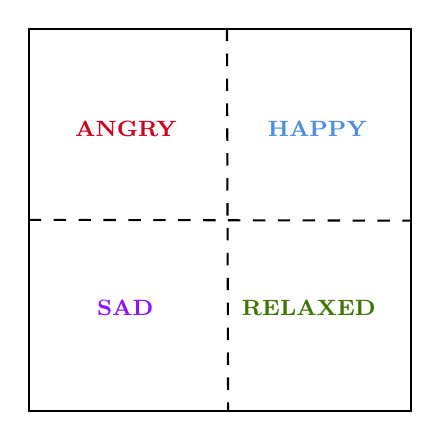
\begin{tikzpicture}[x=0.75pt,y=0.75pt,yscale=-1,xscale=1]
%uncomment if require: \path (0,300); %set diagram left start at 0, and has height of 300


%Shape: Rectangle [id:dp11534307415903555] 
\draw   (148.93,21.48) -- (332.92,21.48) -- (332.92,205.47) -- (148.93,205.47) -- cycle ;
%Straight Lines [id:da7440202322498375] 
\draw  [dash pattern={on 4.5pt off 4.5pt}]  (244.26,21.2) -- (244.82,205.76) ;
%Straight Lines [id:da9738201325291478] 
\draw  [dash pattern={on 4.5pt off 4.5pt}]  (148.75,113.27) -- (332.79,113.69) ;

% Text Node
\draw (169.67,64.48) node [anchor=north west][inner sep=0.75pt]  [font=\footnotesize] [align=left] {\textcolor[rgb]{0.82,0.01,0.11}{\textbf{ANGRY}}};
% Text Node
\draw (262.5,64.48) node [anchor=north west][inner sep=0.75pt]  [font=\footnotesize] [align=left] {\textcolor[rgb]{0.29,0.56,0.89}{\textbf{HAPPY}}};
% Text Node
\draw (180.17,150.48) node [anchor=north west][inner sep=0.75pt]  [font=\footnotesize] [align=left] {\textbf{\textcolor[rgb]{0.56,0.07,1}{SAD}}};
% Text Node
\draw (250,150.48) node [anchor=north west][inner sep=0.75pt]  [font=\footnotesize,color={rgb, 255:red, 65; green, 117; blue, 5 }  ,opacity=1 ] [align=left] {\textbf{RELAXED}};


\end{tikzpicture}

        \fonte{Author.}
\end{figure}

% A Figura \ref{fig:EmocardsMethod} apresenta o método Emocards inserido no Circumplexo de Afeto de Russel, mostrando os oito (8) octantes distribuídos nos quatro (4) estados de espírito, e com as dezesseis (16) representações gráficas associadas a eles. 
Figure \ref{fig:EmocardsMethod} presents the Emocards method inserted in Russell's Circumplex of Affection, showing the eight (8) octants distributed in the four (4) states of mind and with the sixteen (16) graphic representations associated with them.

\begin{figure}[!htb]
        \centering
        \caption{Emocards method and its eight categories within Russell's Circumplex.}
        \label{fig:EmocardsMethod}
        \includegraphics[width=0.5\textwidth]{img/Emocards.png}
        \fonte{\cite{Reijneveld:2003}.}
\end{figure}

% A execução se deu em dezembro de 2021, ainda sem oferecer acesso aos participantes para que eles avaliassem os artefados produzidos pelos geradores implementados em ambas as ferramentas.
% Em relação aos geradores da ERtext, os mesmos foram desativados dentro do ambiente controlado que distribuído.
% Para os geradores da brModelo foi apenas orientado que não era necessário fazer a transformação do modelo conceitual para o lógico ou físico. 
% Isso se deu em razão de tentarmos replicar o experimento anterior visando comparar resultados e, por conta do tempo disponível ser limitado, isso poderia tornar somar mais uma ameaça aos resultados, já que demandaria mais esforço para realizar as tarefas adicionais.
The execution took place in December 2021, still without offering access to the participants so that they could evaluate the artifacts produced by the generators implemented in both tools.
On the one hand, regarding the ERtext generators, we deactivated them within the controlled environment that we distributed.
%Regarding the ERtext generators, they were deactivated within the controlled environment that was distributed.
On the other hand, for the brModelo generators, we only advised that it was not required to transform the conceptual model into a logical or physical one.
%For the brModelo generators, it was only advised that it was not necessary to transform the conceptual model into a logical or physical one.
Hence, this has happened because we tried to replicate the previous experiment to compare the results. 
Also, given the limited time available, this could add another threat to the results, as it would require more effort to perform the additional tasks.
%This was due to the fact that we tried to replicate the previous experiment in order to compare results and, due to the limited time available, this could add another threat to the results, as it would require more effort to perform the additional tasks.

%###########################################################
\subsubsection{Results Analysis}
%###########################################################

% Esta seção apresenta os resultados obtidos da execução do \ac{ex2}.
% Os dados utilizados estão disponíveis em um repositório\footnote{: link do repositório ex2 no Zenodo.} público na plataforma Zenodo.
% Todos os testes estatísticos foram realizados com apoio da linguagem R em conjunto com a IDE RStudio. 
% Os scripts para este experimento estão disponíveis de forma pública em um repositório\footnote{\url{https://github.com/JonnathanRiquelmo/misc/blob/main/some-scripts.r}}, portanto desta forma qualquer pessoa pode, além de consultar todos os dados brutos, executá-los localmente e verificar os resultados.
This section presents the results obtained from the execution of \ac{ex2}.
The data used is available in a public repository\footnote{EX2 repository: https://doi.org/10.5281/zenodo.6416356.} on the Zenodo platform.
All statistical tests were performed with the support of the R language with the IDE RStudio.
The scripts for this experiment are publicly available in a repository\footnote{\url{https://github.com/JonnathanRiquelmo/misc/blob/main/some-scripts.r}}. 
Hence, anyone can run it locally and verify their results beyond also querying all the raw data.
%so this way anyone can, in addition to querying all the raw data, running it locally, and verifying the results.

% Levamos em consideração as mesmas hipóteses anteriores, relacionadas ao esforço (tempo) necessário e efetividade (qualidade) alcançada pelos modelos feitos.
% Para a avaliação referente ao esforço foram utilizados o teste de normalidade Shapiro-Wilk, em razão da amostra ter menos de trinta (30) elementos, e o Teste T pareado para amostras dependentes, em que foi levado em consideração os tempos coletados durante a execução das atividades de modelagem do experimento.
We bore in mind the same previous hypotheses related to the effort (time) needed and effectiveness (quality) achieved by the models created.
%We took into account the same previous hypotheses, related to the effort (time) needed and effectiveness (quality) achieved by the models made.
For the evaluation regarding the effort, once the sample had less than thirty (30) elements, we used the Shapiro-Wilk normality test.
Otherside the paired T-Test for dependent samples, when we considered the effort spent collected during the execution of the modeling activities.
%For the evaluation regarding the effort, the Shapiro-Wilk normality test was used, due to the sample having less than thirty (30) elements, and the paired T Test for dependent samples, in which the times collected during the execution of the modeling activities were taken into account.

% O método Shapiro-Wilk testa a hipótese nula de que uma distribuição é normal, mediante o cálculo do valor $W$, onde após é então verificado na tabela do teste\footnote{\url{ http://www.uel.br/projetos/experimental/pages/arquivos/Probabilidades\_Shapiro.pdf }} se ocorre a rejeição ou aceitação da hipótese. 
% O cálculo do método Shapiro-Wilk é dado conforme a fórmula da Equação \ref{eq:Shapiro}: 
The Shapiro-Wilk method tests the null hypothesis by calculating whether is a normal distribution revealed by the value $W$.
Then we can verify in the test table\footnote{\url{ http://www.uel.br/ projects/experimental/pages/arquivos/probabilities\_Shapiro.pdf }} whether the hypothesis is rejected or accepted.
%The Shapiro-Wilk method tests the null hypothesis that a distribution is normal, by calculating the value $W$, after which it is then verified in the test table\footnote{\url{ http://www.uel.br/ projects/experimental/pages/arquivos/probabilities\_Shapiro.pdf }} if the hypothesis is rejected or accepted.
The calculation of the Shapiro-Wilk method is given according to the formula of Equation \ref{eq:Shapiro}:

\begin{equation}
\label{eq:Shapiro}
%\[ 
W = \frac{\left(\sum_{i=1}^{n} a_ix_{(i)}\right)^2}{\sum_{i=1}^{n}\left(x_i -\overline{x}\right)} 
%\]
\end{equation}

% Uma forma simplificada do Teste T pareado para amostras dependentes
% se dá conforme a fórmula da Equação \ref{eq:TestT}:
A simplified form of the Paired T-Test for dependent samples
is given according to the formula of Equation \ref{eq:TestT}:

\begin{equation}
\label{eq:TestT}
%\[ 
t = \frac{m}{s/\sqrt{n}} 
%\]
\end{equation}

% Nesta fórmula o \textit{\textbf{m}} e o \textit{\textbf{s}} são a média e o desvio padrão da diferença (\textbf{\textit{d}}), respectivamente. 
% O \textit{\textbf{n}} corresponde ao tamanho de \textit{\textbf{d}}, ou seja, o tamanho da amostra.
% Este teste de hipótese é usado para comparar as médias de duas amostras relacionadas, ou seja, quando se possui dois valores (ou pares de valores) para uma mesma amostra. 
% Contudo, para comparar as médias dos dois conjuntos de dados emparelhados, as diferenças entre todos os pares precisaram ser calculadas primeiro.
% O nível de significância alfa ($\alpha$) utilizado foi de cinco por cento (5\%).
In this formula, \textit{\textbf{m}} and \textit{\textbf{s}} are the mean and standard deviation of the difference (\textbf{\textit{d}}), respectively.
The \textit{\textbf{n}} corresponds to the size of \textit{\textbf{d}}, that is, the size of the sample.
We used this hypothesis test to compare the means of two related samples, \textit{i.e.}, when you have two values (or pairs of values) for the same sample.
%This hypothesis test is used to compare the means of two related samples, that is, when you have two values (or pairs of values) for the same sample.
However, to compare the means of the two paired data sets, the differences between all pairs had to be calculated first.
The alpha significance level ($\alpha$) used was five percent (5\%).

% Para os testes da efetividade foram adotados os mesmos métodos estatísticos, porém ao invés do uso da métrica de tempo gasto nas atividades, foi necessário outra grandeza.
% Sendo assim, foram realizados novamente cálculos para uma medida F1, conforme também descrito anteriormente na Seção \ref{ssec_experiments:preliminary_planning}.
We adopted the same statistical methods for the effectiveness tests, but instead of using the effort spent (time) measure on activities, we used another magnitude.
%For the effectiveness tests, the same statistical methods were adopted, but instead of using the metric of time spent on activities, another magnitude was needed.
Therefore, we performed calculations again for an F1 measure, as described previously in Section \ref{ssec_experiments:preliminary_planning}.
%Therefore, calculations were performed again for an F1 measure, as also described previously in Section \ref{ssec_experiments:preliminary_planning}.


% A partir dos valores brutos dos tempos foi calculada a diferença para ser possível realizar o teste de normalidade Shapiro-Wilk.
% Por ser um teste estatístico, esta técnica tem como produto a medida do valor-$p$.
% Para este teste foi adotado um nível de significância $\alpha$~=~5\%. 
% Isso significa que se o valor-$p$ for menor que 5\% ($p$ < 0.05), a hipótese nula de que a distribuição é normal deve ser rejeitada.
From the raw time values, the difference was calculated to be able to perform the Shapiro-Wilk normality test.
As it is a statistical test, this technique has as its product the measure of the $p$-value.
A significance level of $\alpha$~=~5\% was adopted for this test.
Hence, through this, if the $p$-value is less than 5\% ($p$ < 0.05), we must reject the null hypothesis since the distribution is not normal.
%This means that if the $p$-value is less than 5\% ($p$ < 0.05), the null hypothesis that the distribution is normal must be rejected.

% Após os cálculos com o conjunto das diferenças dos tempos chegou-se a um valor-$p$ de 0.5991.
% Como valor-$p$ \textgreater $\alpha$, a hipótese nula foi aceita, concluindo assim que os dados são normalmente distribuídos.
% Em outras palavras, a diferença entre a amostra de dados e a distribuição normal não é grande o suficiente para ser estatisticamente significativa.
After the calculations with the set of time differences, we reached a $p$-value of 0.5991.
As $p$-value \textgreater $\alpha$, we accepted the null hypothesis, thus concluding that the data are a normal distribution.
%As $p$-value \textgreater $\alpha$, the null hypothesis was accepted, thus concluding that the data are normally distributed.
In other words, the difference between the sample data and the normal distribution is not large enough to be statistically significant.

% É importante ressaltar que quanto maior o valor-$p$, mais ele suporta uma hipótese nula. 
% No caso do resultado obtido a chance de erro do tipo 1 (rejeitar uma hipótese nula que é correta) é muito alta, podendo ser traduzida em 59,91\% (0.5991).
% Ainda em relação ao teste de normalidade, o valor de \textit{W} calculado foi de 0.968, estando dentro do intervalo aceito do valor crítico de 95\%. 
% Isto significa que existe 95\% de chances da amostra ter origem em uma população normal.
It is important to note that the higher the $p$-value, the more it supports a null hypothesis.
In the case of the result obtained, the chance of a type 1 error (rejecting a correct null hypothesis) is very high, which we can translate into 59.91\% (0.5991).
%In the case of the result obtained, the chance of a type 1 error (rejecting a null hypothesis that is correct) is very high, which can be translated into 59.91\% (0.5991).
Still, about the normality test, we calculated the value of \textit{W} resulting 0.968, being within the range of the critical value accepted of 95\%.
%Still in relation to the normality test, the value of \textit{W} calculated was 0.968, being within the accepted range of the critical value of 95\%.
So this means that there is a 95\% chance that the sample comes from a  population considered normal.
%This means that there is a 95\% chance that the sample comes from a normal population.

% Tendo sido a amostra testada quanto à sua normalidade, foi possível realizar o teste da primeira hipótese estabelecida neste experimento. 
% No teste T pareado para amostras dependentes foi utilizado um nível de significância $\alpha$~=~5\%, com o qual se chegou a uma medida de 0.3492 para o valor-$p$. 
Once we tested the sample for normality, it was possible to test the first hypothesis established in this experiment.
In the paired T-test for dependent samples, we used a significance level of $\alpha$~=~5\%, which reached a measure of 0.3492 for the $p$-value.

% Por ser um teste bicaudal, ou seja, que inclui uma igualdade na sua hipótese nula, esse valor-$p$ não mostra evidências suficientes para garantir a rejeição da afirmativa de $H_0 : \mu Time_G = \mu Time_T$.
% Em resumo, a média dos valores da abordagem gráfica (brModelo) é considerada similar à média da população da abordagem textual (ERtext).
% Em outras palavras, a diferença entre as médias da brModelo e da ERtext não é grande o suficiente para ser estatisticamente significativa.
% A Figura \ref{fig:boxplotTempo2} exibe um gráfico boxplot com a variação observada dos dados obtidos. 
As it is a two-tailed test, that is, it includes an equality in its null hypothesis, this $p$-value does not show enough evidence to guarantee the rejection of the statement of $H_0 : \mu Time_G = \mu Time_T$.
In short, we considered the average of the values of the graphical approach (brModelo) similar to the textual one (ERtext).
%In short, the average of the values of the graphical approach (brModelo) is considered similar to the average of the population of the textual approach (ERtext).
In other words, the difference between the brModelo and ERtext means is not large enough to be statistically significant.
Figure \ref{fig:boxplotTime2} shows a box-plot with the observed variation of the data obtained.
%Figure \ref{fig:boxplotTime2} displays a box-plot plot with the observed variation of the data obtained.

\begin{figure}[!htb]
        \centering
        \caption{Box-plot - Effort per treatments in EX2.}
        \label{fig:boxplotTempo2}
        \begin{filecontents*}{data2.csv}
24,24,28,28,29,30,30,30,31,33,35,38,38,44,45,46,46,46,53,58,61,70,74,90,102
21,23,25,29,30,30,31,32,35,36,40,40,43,44,47,50,50,55,55,55,67,74,93,93,171
\end{filecontents*}

\makeatletter
\pgfplotsset{
    boxplot/hide outliers/.code={
        \def\pgfplotsplothandlerboxplot@outlier{}%
    }
}
\makeatother

\begin{tikzpicture}
    \pgfplotstableread[col sep=comma]{data2.csv}\csvdata
    % Boxplot groups columns, but we want rows
    \pgfplotstabletranspose\datatransposed{\csvdata} 
    \begin{axis}[
        boxplot/draw direction=y,
        xtick={1, 2},
        ylabel={\scriptsize Time (minutes)},
        xticklabels={{\scriptsize Graphical Treatment}, {\scriptsize Textual Treatment}},
        height=7cm,
        width=10cm,
        % boxplot/draw direction = y,
        % axis x line* = bottom,
        % axis y line = left,
        % enlarge y limits,
        ymajorgrids,
        % xtick = {1, 2},
        % xticklabel style = {align=center, font=\small},
        % xticklabels = {Graphical Treatment, Textual Treatment},
        % ylabel = {Time (minutes)},
        ytick = {15, 30, 45, 60, 75, 90,  105, 120, 135, 150, 165, 180},
        yticklabel style = {font=\scriptsize}
    ]
        \foreach \n in {1,...,2} {
            \addplot+[boxplot, /pgfplots/boxplot/hide outliers, fill, fill opacity=0.4, draw=black] table[y index=\n] {\datatransposed};
        }
    \end{axis}
\end{tikzpicture}


        \fonte{Author.}
\end{figure}

% Para avaliar a hipotése referente a efetividade do uso das abordagens, os artefatos produzidos pelos sujeitos foram avaliados conforme os modelos de referência previamente estabelecidos.
% Como dito, nesta avaliação foi utilizada a medida F1, uma medida proveniente da área de reconhecimento de padrões e recuperação de informação. 
% Essa medida representa a combinação da precisão e revocabilidade observada de um resultado em relação à uma referência.
To assess the hypothesis regarding the effectiveness of using the approaches, we analyzed the artifacts produced by the subjects according to the previously established reference models.
As mentioned, we used in this evaluation the F1 measure, this measure from the area of pattern recognition and information retrieval.
This measure represents the combination of the accuracy observed and the recallability of a result against a reference.

% Após a obtenção dos valores F1 de cada modelo, foi realizado o teste de normalidade Shapiro-Wilk.
% Após os cálculos com o conjunto das diferenças da medida F1 de cada modelo, chegou-se a um valor-$p$ de 0.5166.
% Com este resultado obtido a chance de erro do tipo 1 (rejeitar uma hipótese nula que é correta) pode ser muito alta, podendo ser traduzida em 51,66\% (0.5166).
After obtaining the F1 values of each model, we performed the Shapiro-Wilk normality test.
After the calculations with the set of differences of the F1 measure of each model, we reached a $p$-value of 0.5166.
With this result obtained, the chance of a type 1 error (rejecting a correct null hypothesis) can be very high, which we can translate into 51.66\% (0.5166).

% Como o valor-$p$ \textgreater $\alpha$, a hipótese nula foi aceita, constatando assim que os dados são normalmente distribuídos, isto é, a diferença entre a amostra de dados e uma distribuição normal não é grande o suficiente para ser estatisticamente significativa.
As the value-$p$ \textgreater $\alpha$, we accepted the null hypothesis, thus noting that the data are a normal distribution, \textit{i.e.}, the difference between the sample of data and normal distribution is not large enough to be statistically significant.
%As the value-$p$ \textgreater $\alpha$, the null hypothesis was accepted, thus noting that the data are normally distributed, that is, the difference between the sample of data and a normal distribution is not large enough to be statistically significant.

% Após a amostra ser testada quanto à sua normalidade, foi realizado o teste da segunda hipótese definida, relativa a efetividade (qualidade) das abordagens. 
% Desta vez, no teste T pareado para amostra dependentes, novamente foi utilizado um nível de significância $\alpha$~=~5\%, com o qual se chegou a uma medida de 0.2147 para o valor-$p$. 
After we tested the sample for normality, we performed the test of the second hypothesis defined concerning the effectiveness (quality) of the approaches.
%After the sample was tested for normality, the test of the second defined hypothesis was performed, concerning the effectiveness (quality) of the approaches.
This time, in the paired T-test for dependent samples, we used a significance level $\alpha$~=~5\% again, with which we reached a measure of 0.2147 for the $p$-value.
%This time, in the paired T-test for dependent samples, a significance level $\alpha$~=~5\% was used again, with which a measure of 0.2147 was reached for the $p$-value.

% Pela afirmativa original incluir uma igualdade, caracterizando também este teste como bicaudal, chegou-se a conclusão que o valor-$p$ calculado demonstra que não há evidências suficientes para garantir a rejeição da afirmativa da hipótese nula original, denotada como $H_0 : \mu Effectiveness_G = \mu Effectiveness_T$.
% Logo, a hipótese nula de que as abordagens possuem efetividades iguais é aceita, pois segundo o teste a diferença média da medida F1 entre os tratamentos não é estatisticamente significativa.
% A Figura \ref{tab:ResultsModelosGeral2} apresenta as medidas médias dos valores avaliados, e também fornecem a possibilidade para a realização de uma análise de dispersão.
By the original statement including equality, also characterizing this test as two-tailed, we concluded that the calculated $p$-value demonstrates that there is not enough evidence to guarantee the rejection of the statement of the original null hypothesis, denoted as $H_0 : \mu Effectiveness_G = \mu Effectiveness_T$.
%By the original statement including an equality, also characterizing this test as two-tailed, it was concluded that the calculated value-$p$ demonstrates that there is not enough evidence to guarantee the rejection of the statement of the original null hypothesis, denoted as $H_0 : \mu Effectiveness_G = \mu Effectiveness_T$.
Therefore, we accepted the null hypothesis that the approaches have equal effectiveness because, in accord with the test, the mean difference of the F1 measure between the treatments is not statistically significant.
%Therefore, the null hypothesis that the approaches have equal effectiveness is accepted, because according to the test, the mean difference of the F1 measure between the treatments is not statistically significant.
Table \ref{tab:ResultsModelosGeral2} presents the basic statistical measures of the values evaluated, providing means for dispersion analysis.
%Table \ref{tab:ResultsModelosGeral2} presents the average measures of the evaluated values, and also provides the possibility to carry out a dispersion analysis.

\rowcolors{1}{gray!15}{white}
\begin{table}[!htb]
    \caption{Measures of the conceptual data models produced in EX2.}
    \label{tab:ResultsModelosGeral2}
    \centering
    % \scriptsize
    \tiny
    \begin{tabular}{l|ccccc|ccccc}%{l|ccccc|ccccc}
    \bottomrule
    \rowcolor[HTML]{C0C0C0}
    \multicolumn{1}{l}{} &
    \multicolumn{5}{c|}{\textbf{Graphical Treatment}} &
    \multicolumn{5}{c}{\textbf{Textual Treatment}}
    \\ 
    \hline
    \rowcolor[HTML]{C0C0C0}
    \textbf{Measure} & \textbf{MI} & \textbf{RI} & \textbf{P(\%)} & \textbf{R(\%)} & \textbf{F1(\%)} &
    \textbf{MI} & \textbf{RI} & \textbf{P(\%)} & \textbf{R(\%)} & \textbf{F1(\%)}
    \\
    \hline
Maximum	&	49.00	&	44.00	&	93.75	&	92.50	&	91.67	&	65.00	&	45.00	&	94.74	&	92.68	&	91.14	\\
3\textdegree Quartile	&	46.00	&	39.00	&	88.89	&	85.42	&	86.02	&	47.00	&	38.00	&	89.19	&	87.80	&	87.06	\\
Average	&	41.08	&	35.20	&	85.88	&	78.57	&	81.74	&	44.64	&	36.48	&	83.24	&	83.35	&	82.81	\\
Median	&	43.00	&	36.00	&	86.05	&	77.50	&	81.32	&	44.00	&	36.00	&	85.37	&	83.67	&	84.71	\\
1\textdegree Quartile	&	36.00	&	31.00	&	84.78	&	75.00	&	79.12	&	40.00	&	34.00	&	81.82	&	79.59	&	78.72	\\
Minimum	&	27.00	&	23.00	&	71.43	&	57.50	&	68.66	&	34.00	&	32.00	&	58.46	&	69.39	&	69.47	\\
Variance	&	34.63	&	23.84	&	20.21	&	72.57	&	26.91	&	59.59	&	10.25	&	102.43	&	34.72	&	37.18	\\
SD	&	5.89	&	4.88	&	4.50	&	8.52	&	5.19	&	7.72	&	3.20	&	10.12	&	5.89	&	6.10	\\
    \toprule
\end{tabular}
\begin{tablenotes}
    \scriptsize
    \centering
    \item \textit{Legend: MI = Modeled Items; RI = Relevant Items; P = Precision; \\R = Recall; F1 = F1-Score; SD = Standard Deviation.}
\end{tablenotes}
\fonte{Author.}
\end{table}

% O gráfico boxplot da Figura \ref{fig:boxplotMedidaF2} exibe uma representação visual da medida F1 dos tratamentos aplicados.
% Com base neste gráfico é possível verificar o resultado obtido no teste de hipótese pois a dispersão dos dados não apresenta grande diferença entre as abordagens. 
The box-plot in Figure \ref{fig:boxplotMeasureF2} shows a visual representation of the F1 measurement of the treatments applied.
Based on this graph, it is possible to verify the result obtained in the hypothesis test, as the data dispersion does not present a high difference between the approaches.

\begin{figure}[!htb]
        \centering
        \caption{Box-plot - F1 per treatments in EX2.}
        \label{fig:boxplotMeasureF2}
        \include{img/boxplotMedidaF2}
        \fonte{Author.}
\end{figure}

% A avaliação referente aos atributos de qualidade para as ferramentas é apresentado na Figura \ref{fig:inst3GERALExp2}.
% No geral, o resultado da avaliação feita pelos participantes foi proporcionalmente similar a obtida no experimento anterior. 
% Os destaques desta vez ficaram por conta do atributo de satisfação para a abordagem textual, enquanto os atributos de conformidade e compreensão se sairam melhores na abordagem gráfica. 
% Outro ponto a ser ressaltado é a diferença levemente menor no atributo de produtividade, mas ainda se mantendo em favor da abordagem textual.
Figure~\ref{fig:inst3GERALExp2} shows the evaluation regarding the quality attributes of the tools.
%The evaluation regarding the quality attributes for the tools is shown in Figure~\ref{fig:inst3GERALExp2}.
In general, the evaluation results made by the participants were proportionally similar to that obtained in the previous experiment.
%In general, the result of the evaluation made by the participants was proportionally similar to that obtained in the previous experiment.
The highlights this time was the Satisfaction attribute for the textual approach, while the Conformity and Understanding attributes performed better in the graphical one.
%The highlights this time was the satisfaction attribute for the textual approach, while the conformity and understanding attributes performed better in the graphical approach.
Another point to highlight is the slightly smaller difference in the Productivity attribute, but still in favor of the textual approach.
%Another point to be highlighted is the slightly smaller difference in the productivity attribute, but still in favor of the textual approach.

\begin{figure}[!htb]
    \centering
    \caption{Quality attributes per treatments in EX2.}
    \label{fig:inst3GERALExp2}
    \include{img/Inst3_2}
    \fonte{Author.}
\end{figure}

% A avaliação referente aos construtores da DSL da abordagem textual, os resultados também seguiram a mesma proporção observada no primeiro experimento.
% Isso nos leva a concluir que de fato é necessário, principalmente, uma reavaliação da representação dos relacionamentos ternários para torná-los mais fáceis de aprender, interpretar e utilizar.
The evaluation results referring to the DSL builders of the textual approach also followed the same proportion observed in the first experiment.
%The evaluation referring to the DSL builders of the textual approach, the results also followed the same proportion observed in the first experiment.
Then leads us to conclude that it is necessary, mainly, to re-execute an evaluation of the representation of the ternary relationships to make them easier to learn, interpret, and use.
%This leads us to conclude that, in fact, it is necessary, mainly, a reassessment of the representation of ternary relationships to make them easier to learn, interpret and use.

\begin{figure}[!htb]
    \centering
    \caption{Evaluation of DSL designers in EX2.}
    \label{fig:inst4GERALExp2}
    \pgfplotsset{testbar/.style={
            xbar stacked,
            legend cell align=left,
            legend style={
                legend columns=6,
                font=\scriptsize,
                at={(xticklabel cs:1.0)},
                anchor=north east,
                draw=none
                },
            width=10cm,
            axis y line*= none, 
            axis x line*= bottom,
            xmajorgrids = false,
            xmin=0,xmax=25,
            ytick = data,
            yticklabels = {
            {\scriptsize Entity}, 
            {\scriptsize Referential Attribute},
            {\scriptsize Descriptive Attribute},
            {\scriptsize Binary Relationship},
            {\scriptsize Ternary Relationship}, 
            {\scriptsize Self-relationship},
            {\scriptsize Cardinality},
            {\scriptsize Generalization}
            },
            tick align = outside, 
            xticklabel style = {font=\scriptsize},
            xtick pos = left,
             bar width=3.5mm, 
             y=6.5mm,
             enlarge y limits={abs=0.450},% 0.5 + 0.5*(y - bar width)/y [TeX.sx #47995] #47995]
            nodes near coords,
            nodes near coords align=center,%Move values in bar
            every node near coord/.append style={
                black,
                font=\scriptsize,
                text opacity=1,
                fill=white,
                fill opacity=0.5,
                outer sep=\pgflinewidth
            }
        }}
    \begin{tikzpicture}
    \begin{axis}[testbar] 
    \addplot[pattern color=red,pattern=north east lines] coordinates
        {(0,8)(0,7)(0,6)(0,5)(0,4)(0,3)(0,2)(0,1)};
    \addplot[pattern color=teal,pattern=vertical lines] coordinates
        {(0,8)(0,7)(0,6)(1,5)(2,4)(1,3)(0,2)(0,1)};   
    \addplot[pattern color=gray, pattern=grid] coordinates
        {(0,8)(0,7)(2,6)(2,5)(5,4)(0,3)(0,2)(3,1)};   
    \addplot[pattern color=magenta, pattern=north west lines] coordinates
        {(3,8)(4,7)(2,6)(0,5)(6,4)(3,3)(0,2)(3,1)};   
    \addplot[pattern color=blue, pattern=horizontal lines] coordinates
        {(4,8)(4,7)(6,6)(11,5)(7,4)(5,3)(5,2)(6,1)}; 
    \addplot[pattern color=green, pattern=crosshatch dots] coordinates
        {(18,8)(17,7)(15,6)(11,5)(5,4)(16,3)(20,2)(13,1)};
    \legend{1-Disagree, 2, 3, 4, 5, 6-Agree}
    \end{axis}
    \end{tikzpicture}

% \begin{figure}[!ht]
% \centering
% \caption{Resultados do formulários de avaliação.}
% \begin{tikzpicture}
% \begin{axis}[
%     xbar stacked,
%     legend cell align=center,
%     legend style={
%     legend columns=5,
%         at={(xticklabel cs:1.0)},
%         anchor=north east,
%         draw=none
%     },
%     ytick=data,
%     axis y line*=none,
%     axis x line*=bottom,
%     tick label style={font=\small},
%     legend style={font=\small},
%     label style={font=\small},
%     xtick={0,5,10},
%     xticklabel= {},
%     bar width=7mm,
%     ylabel={Formulário/Grupo},
%     yticklabels={F1-C, F1-E, F2-C, F2-E, F3-C, F3-E},
%     xmin=0,
%     xmax=10,
%     area legend,
%     y=9mm,
%     enlarge y limits={abs=0.825},
%     nodes near coords,
%     nodes near coords align=center,
%     every node near coord/.append style={
%         black,
%         font=\small,
%         text opacity=.65,
%         fill=white,
%         fill opacity=0.6,
%         outer sep=\pgflinewidth
%     }
% ]
% %NOTA 1
% \addplot[pattern color=red,pattern=horizontal lines] coordinates
% {(0,6)(0,5)(0,4)(0,3)(0,2)(0,1)};
% %NOTA 2
% \addplot[pattern color=orange,pattern=grid] coordinates
% {(1,6)(1,5)(1,4)(0,3)(1,2)(0,1)};   
% \addplot[pattern color = green, pattern=crosshatch dots] coordinates
% % NOTA 3
% {(3,6)(3,5)(5,4)(2,3)(5,2)(1,1)};   
% \addplot[pattern color=blue, pattern =vertical lines ] coordinates
% %NOTA 4
% {(2,6)(3,5)(1,4)(4,3)(3,2)(3,1)};   
% \addplot[pattern color=gray, pattern = dots] coordinates
% %NOTA 5
% {(3,6)(3,5)(2,4)(4,3)(0,2)(6,1)};   
% \legend{1-Disagree, 2, 3, 4, 5-Agree}

% \end{axis}
% \end{tikzpicture}
% \footnotesize
% \label{img:respostas1}
% 	\fonte{O autor.}
% \end{figure}
    \fonte{Author.}
\end{figure}

% Finalmente, chegamos aos instrumentos adicionados para tentar verificar o estado de espírito, ou as emoções causadas, pela execução das atividades com cada abordagem.
% Os resultados das avaliações são dispostas em um circumplexo de Russell.
% É possível observar que em relação ao uso da abordagem textual com a ferramenta ERtext houve uma concentração maior nos quadrantes que dizem respeito aos sentimento de alegria (octantes 1 e 2) e relaxamento (octantes 3 e 4).
Finally, we come to the added instruments trying to verify the state of mind or the emotions caused by the execution of the activities with each approach.
%Finally, we come to the added instruments to try to verify the state of mind, or the emotions caused, by the execution of the activities with each approach.
We arranged the results of the evaluations in Russell's Circumplex. 
%The results of the evaluations are arranged in a Russell circumplex. 
It is possible to observe that regarding the use of the textual approach with the ERtext tool, there was a greater concentration in the quadrants that concern feelings of happiness (Octants 1 and 2) and relaxation (Octants 3 and 4).

% Esses dois quadrantes concentraram um total de vinte (20) respondentes.
% Ainda, houve a distribuição de três (3) partipantes que expressaram sentimentos relacionados a tristeza (octantes 5 e 6), e dois (2) sujeitos que demonstraram se identificarem com os Emocards relacionados ao quadrante que diz respeito a emoções de irritabilidade (octantes 7 e 8).
% A Figura \ref{fig:Emocards1_alt} apresenta a distribuição dos sujeitos por cada octante previsto no método Emocards, e que utilizaram a abordagem textual.
These two quadrants concentrated a total of twenty (20) respondents.
Also, there were a distribution of three (3) participants who expressed feelings related to sadness (Octants 5 and 6) and two (2) subjects who demonstrated identification with the Emocards related to the quadrant that concerns emotions of irritability (Octants 7 and 8).
Figure \ref{fig:Emocards1_alt} presents the distribution of subjects for each octant predicted in the Emocards method, which used the textual approach.

\begin{figure}[!htb]
    \centering
    \caption{EX2 Emocards - ERtext.}
    \label{fig:Emocards1_alt}
    

\tikzset{every picture/.style={line width=0.75pt}} %set default line width to 0.75pt        

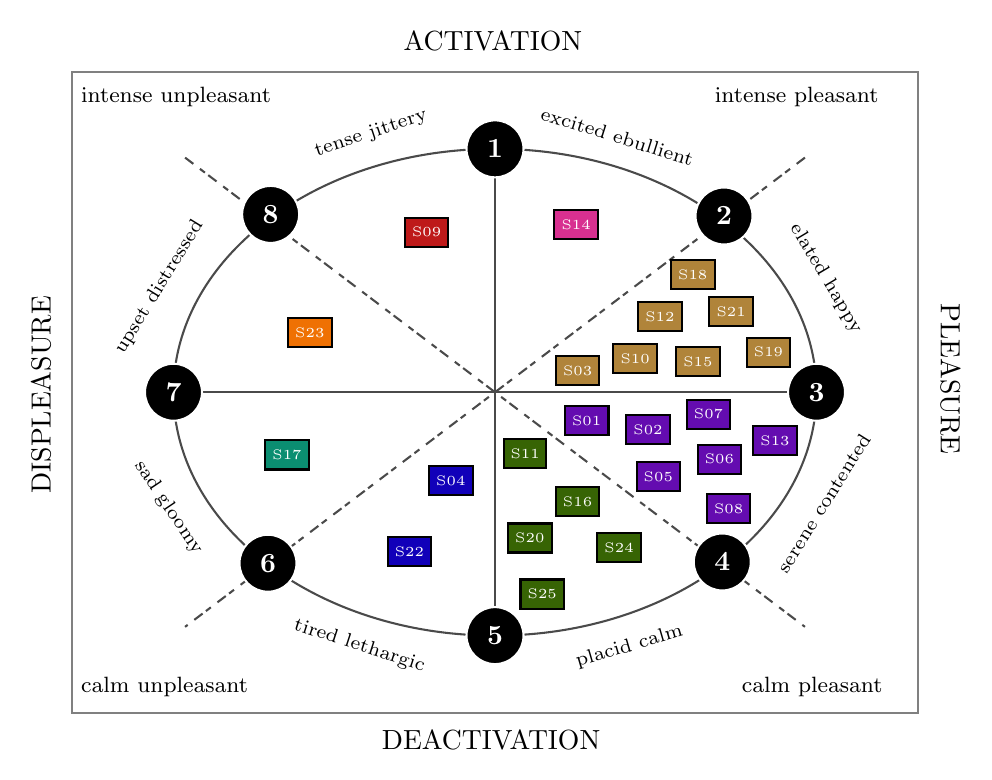
\begin{tikzpicture}[x=0.75pt,y=0.75pt,yscale=-1,xscale=1]
%uncomment if require: \path (0,389); %set diagram left start at 0, and has height of 389

%Flowchart: Or [id:dp3592995680476845] 
\draw  [color={rgb, 255:red, 74; green, 74; blue, 74 }  ,draw opacity=1 ] (182.64,181.1) .. controls (182.64,116.34) and (252,63.84) .. (337.55,63.84) .. controls (423.11,63.84) and (492.46,116.34) .. (492.46,181.1) .. controls (492.46,245.86) and (423.11,298.36) .. (337.55,298.36) .. controls (252,298.36) and (182.64,245.86) .. (182.64,181.1) -- cycle ; \draw  [color={rgb, 255:red, 74; green, 74; blue, 74 }  ,draw opacity=1 ] (182.64,181.1) -- (492.46,181.1) ; \draw  [color={rgb, 255:red, 74; green, 74; blue, 74 }  ,draw opacity=1 ] (337.55,63.84) -- (337.55,298.36) ;
%Straight Lines [id:da30798451784186187] 
\draw [color={rgb, 255:red, 74; green, 74; blue, 74 }  ,draw opacity=1 ] [dash pattern={on 3.75pt off 3pt on 2.25pt off 1.5pt}]  (188.22,68.06) -- (486.88,294.14) ;
%Straight Lines [id:da7804870395610348] 
\draw [color={rgb, 255:red, 74; green, 74; blue, 74 }  ,draw opacity=1 ] [dash pattern={on 3.75pt off 3pt on 2.25pt off 1.5pt}]  (486.88,68.06) -- (188.22,294.14) ;
%Shape: Rectangle [id:dp23344423808181314] 
\draw  [color={rgb, 255:red, 128; green, 128; blue, 128 }  ,draw opacity=1 ] (133.68,26.77) -- (541.42,26.77) -- (541.42,335.43) -- (133.68,335.43) -- cycle ;

% Text Node
\draw  [color={rgb, 255:red, 0; green, 0; blue, 0 }  ,draw opacity=1 ][fill={rgb, 255:red, 100; green, 12; blue, 176 }  ,fill opacity=1 ]  (400.79,192.22) -- (421.79,192.22) -- (421.79,206.22) -- (400.79,206.22) -- cycle  ;
\draw (411.29,199.22) node  [font=\tiny,color={rgb, 255:red, 255; green, 255; blue, 255 }  ,opacity=1 ] [align=left] {S02};
% Text Node
\draw  [color={rgb, 255:red, 0; green, 0; blue, 0 }  ,draw opacity=1 ][fill={rgb, 255:red, 55; green, 100; blue, 4 }  ,fill opacity=1 ]  (342.09,203.64) -- (362.09,203.64) -- (362.09,217.64) -- (342.09,217.64) -- cycle  ;
\draw (352.09,210.64) node  [font=\tiny,color={rgb, 255:red, 255; green, 255; blue, 255 }  ,opacity=1 ] [align=left] {S11};
% Text Node
\draw  [color={rgb, 255:red, 0; green, 0; blue, 0 }  ,draw opacity=1 ][fill={rgb, 255:red, 176; green, 132; blue, 58 }  ,fill opacity=1 ]  (366.87,163.61) -- (387.87,163.61) -- (387.87,177.61) -- (366.87,177.61) -- cycle  ;
\draw (377.37,170.61) node  [font=\tiny,color={rgb, 255:red, 255; green, 255; blue, 255 }  ,opacity=1 ] [align=left] {S03};
% Text Node
\draw  [color={rgb, 255:red, 0; green, 0; blue, 0 }  ,draw opacity=1 ][fill={rgb, 255:red, 100; green, 12; blue, 176 }  ,fill opacity=1 ]  (461.95,197.33) -- (482.95,197.33) -- (482.95,211.33) -- (461.95,211.33) -- cycle  ;
\draw (472.45,204.33) node  [font=\tiny,color={rgb, 255:red, 255; green, 255; blue, 255 }  ,opacity=1 ] [align=left] {S13};
% Text Node
\draw  [color={rgb, 255:red, 0; green, 0; blue, 0 }  ,draw opacity=1 ][fill={rgb, 255:red, 183; green, 0; blue, 0 }  ,fill opacity=0.9 ]  (294.12,96.99) -- (315.12,96.99) -- (315.12,110.99) -- (294.12,110.99) -- cycle  ;
\draw (304.62,103.99) node  [font=\tiny,color={rgb, 255:red, 255; green, 255; blue, 255 }  ,opacity=1 ] [align=left] {S09};
% Text Node
\draw  [color={rgb, 255:red, 0; green, 0; blue, 0 }  ,draw opacity=1 ][fill={rgb, 255:red, 100; green, 12; blue, 176 }  ,fill opacity=1 ]  (371.22,187.92) -- (392.22,187.92) -- (392.22,201.92) -- (371.22,201.92) -- cycle  ;
\draw (381.72,194.92) node  [font=\tiny,color={rgb, 255:red, 255; green, 255; blue, 255 }  ,opacity=1 ] [align=left] {S01};
% Text Node
\draw  [color={rgb, 255:red, 0; green, 0; blue, 0 }  ,draw opacity=1 ][fill={rgb, 255:red, 100; green, 12; blue, 176 }  ,fill opacity=1 ]  (405.75,214.64) -- (426.75,214.64) -- (426.75,228.64) -- (405.75,228.64) -- cycle  ;
\draw (416.25,221.64) node  [font=\tiny,color={rgb, 255:red, 255; green, 255; blue, 255 }  ,opacity=1 ] [align=left] {S05};
% Text Node
\draw  [color={rgb, 255:red, 0; green, 0; blue, 0 }  ,draw opacity=1 ][fill={rgb, 255:red, 17; green, 0; blue, 185 }  ,fill opacity=1 ]  (305.76,216.61) -- (326.76,216.61) -- (326.76,230.61) -- (305.76,230.61) -- cycle  ;
\draw (316.26,223.61) node  [font=\tiny,color={rgb, 255:red, 255; green, 255; blue, 255 }  ,opacity=1 ] [align=left] {S04};
% Text Node
\draw  [color={rgb, 255:red, 0; green, 0; blue, 0 }  ,draw opacity=1 ][fill={rgb, 255:red, 176; green, 132; blue, 58 }  ,fill opacity=1 ]  (424.83,159.33) -- (445.83,159.33) -- (445.83,173.33) -- (424.83,173.33) -- cycle  ;
\draw (435.33,166.33) node  [font=\tiny,color={rgb, 255:red, 255; green, 255; blue, 255 }  ,opacity=1 ] [align=left] {S15};
% Text Node
\draw  [color={rgb, 255:red, 0; green, 0; blue, 0 }  ,draw opacity=1 ][fill={rgb, 255:red, 100; green, 12; blue, 176 }  ,fill opacity=1 ]  (435.18,206.39) -- (456.18,206.39) -- (456.18,220.39) -- (435.18,220.39) -- cycle  ;
\draw (445.68,213.39) node  [font=\tiny,color={rgb, 255:red, 255; green, 255; blue, 255 }  ,opacity=1 ] [align=left] {S06};
% Text Node
\draw  [color={rgb, 255:red, 0; green, 0; blue, 0 }  ,draw opacity=1 ][fill={rgb, 255:red, 100; green, 12; blue, 176 }  ,fill opacity=1 ]  (439.6,230.11) -- (460.6,230.11) -- (460.6,244.11) -- (439.6,244.11) -- cycle  ;
\draw (450.1,237.11) node  [font=\tiny,color={rgb, 255:red, 255; green, 255; blue, 255 }  ,opacity=1 ] [align=left] {S08};
% Text Node
\draw  [color={rgb, 255:red, 0; green, 0; blue, 0 }  ,draw opacity=1 ][fill={rgb, 255:red, 176; green, 132; blue, 58 }  ,fill opacity=1 ]  (394.61,157.99) -- (415.61,157.99) -- (415.61,171.99) -- (394.61,171.99) -- cycle  ;
\draw (405.11,164.99) node  [font=\tiny,color={rgb, 255:red, 255; green, 255; blue, 255 }  ,opacity=1 ] [align=left] {S10};
% Text Node
\draw  [color={rgb, 255:red, 0; green, 0; blue, 0 }  ,draw opacity=1 ][fill={rgb, 255:red, 207; green, 0; blue, 118 }  ,fill opacity=0.81 ]  (366.18,93.21) -- (387.18,93.21) -- (387.18,107.21) -- (366.18,107.21) -- cycle  ;
\draw (376.68,100.21) node  [font=\tiny,color={rgb, 255:red, 255; green, 255; blue, 255 }  ,opacity=1 ] [align=left] {S14};
% Text Node
\draw  [color={rgb, 255:red, 0; green, 0; blue, 0 }  ,draw opacity=1 ][fill={rgb, 255:red, 176; green, 132; blue, 58 }  ,fill opacity=1 ]  (406.53,137.78) -- (427.53,137.78) -- (427.53,151.78) -- (406.53,151.78) -- cycle  ;
\draw (417.03,144.78) node  [font=\tiny,color={rgb, 255:red, 255; green, 255; blue, 255 }  ,opacity=1 ] [align=left] {S12};
% Text Node
\draw  [color={rgb, 255:red, 0; green, 0; blue, 0 }  ,draw opacity=1 ][fill={rgb, 255:red, 100; green, 12; blue, 176 }  ,fill opacity=1 ]  (429.94,184.66) -- (450.94,184.66) -- (450.94,198.66) -- (429.94,198.66) -- cycle  ;
\draw (440.44,191.66) node  [font=\tiny,color={rgb, 255:red, 255; green, 255; blue, 255 }  ,opacity=1 ] [align=left] {S07};
% Text Node
\draw  [color={rgb, 255:red, 255; green, 255; blue, 255 }  ,draw opacity=1 ][fill={rgb, 255:red, 0; green, 0; blue, 0 }  ,fill opacity=1 ]  (337.55, 63.84) circle [x radius= 13.73, y radius= 13.73]   ;
\draw (337.55,63.84) node  [font=\normalsize,color={rgb, 255:red, 255; green, 255; blue, 255 }  ,opacity=1 ] [align=left] {\textbf{1}};
% Text Node
\draw  [color={rgb, 255:red, 255; green, 255; blue, 255 }  ,draw opacity=1 ][fill={rgb, 255:red, 0; green, 0; blue, 0 }  ,fill opacity=1 ]  (447.88, 96.18) circle [x radius= 13.73, y radius= 13.73]   ;
\draw (447.88,96.18) node  [font=\normalsize,color={rgb, 255:red, 255; green, 255; blue, 255 }  ,opacity=1 ] [align=left] {\textbf{2}};
% Text Node
\draw  [color={rgb, 255:red, 255; green, 255; blue, 255 }  ,draw opacity=1 ][fill={rgb, 255:red, 0; green, 0; blue, 0 }  ,fill opacity=1 ]  (492.46, 181.1) circle [x radius= 13.73, y radius= 13.73]   ;
\draw (492.46,181.1) node  [font=\normalsize,color={rgb, 255:red, 255; green, 255; blue, 255 }  ,opacity=1 ] [align=left] {\textbf{3}};
% Text Node
\draw  [color={rgb, 255:red, 255; green, 255; blue, 255 }  ,draw opacity=1 ][fill={rgb, 255:red, 0; green, 0; blue, 0 }  ,fill opacity=1 ]  (447.05, 262.88) circle [x radius= 13.73, y radius= 13.73]   ;
\draw (447.05,262.88) node  [font=\normalsize,color={rgb, 255:red, 255; green, 255; blue, 255 }  ,opacity=1 ] [align=left] {\textbf{4}};
% Text Node
\draw  [color={rgb, 255:red, 255; green, 255; blue, 255 }  ,draw opacity=1 ][fill={rgb, 255:red, 0; green, 0; blue, 0 }  ,fill opacity=1 ]  (337.55, 298.36) circle [x radius= 13.73, y radius= 13.73]   ;
\draw (337.55,298.36) node  [font=\normalsize,color={rgb, 255:red, 255; green, 255; blue, 255 }  ,opacity=1 ] [align=left] {\textbf{5}};
% Text Node
\draw  [color={rgb, 255:red, 255; green, 255; blue, 255 }  ,draw opacity=1 ][fill={rgb, 255:red, 0; green, 0; blue, 0 }  ,fill opacity=1 ]  (228.16, 263.49) circle [x radius= 13.73, y radius= 13.73]   ;
\draw (228.16,263.49) node  [font=\normalsize,color={rgb, 255:red, 255; green, 255; blue, 255 }  ,opacity=1 ] [align=left] {\textbf{6}};
% Text Node
\draw  [color={rgb, 255:red, 255; green, 255; blue, 255 }  ,draw opacity=1 ][fill={rgb, 255:red, 0; green, 0; blue, 0 }  ,fill opacity=1 ]  (182.64, 181.1) circle [x radius= 13.73, y radius= 13.73]   ;
\draw (182.64,181.1) node  [font=\normalsize,color={rgb, 255:red, 255; green, 255; blue, 255 }  ,opacity=1 ] [align=left] {\textbf{7}};
% Text Node
\draw  [color={rgb, 255:red, 255; green, 255; blue, 255 }  ,draw opacity=1 ][fill={rgb, 255:red, 0; green, 0; blue, 0 }  ,fill opacity=1 ]  (229.45, 95.43) circle [x radius= 13.73, y radius= 13.73]   ;
\draw (229.45,95.43) node  [font=\normalsize,color={rgb, 255:red, 255; green, 255; blue, 255 }  ,opacity=1 ] [align=left] {\textbf{8}};
% Text Node
\draw (112.89,231.39) node [anchor=north west][inner sep=0.75pt]  [rotate=-270] [align=left] {DISPLEASURE};
% Text Node
\draw (292.08,5.96) node [anchor=north west][inner sep=0.75pt]   [align=left] {ACTIVATION};
% Text Node
\draw (281.58,342.71) node [anchor=north west][inner sep=0.75pt]   [align=left] {DEACTIVATION};
% Text Node
\draw (562.94,136.89) node [anchor=north west][inner sep=0.75pt]  [rotate=-90] [align=left] {PLEASURE};
% Text Node
\draw (150.9,160.23) node [anchor=north west][inner sep=0.75pt]  [font=\scriptsize,rotate=-301.49] [align=left] {upset distressed};
% Text Node
\draw (247.79,60.45) node [anchor=north west][inner sep=0.75pt]  [font=\scriptsize,rotate=-341.6] [align=left] {tense jittery};
% Text Node
\draw (359.94,41.46) node [anchor=north west][inner sep=0.75pt]  [font=\scriptsize,rotate=-17.34] [align=left] {excited ebullient};
% Text Node
\draw (485.75,96.5) node [anchor=north west][inner sep=0.75pt]  [font=\scriptsize,rotate=-59.2] [align=left] {elated happy};
% Text Node
\draw (470.66,265.95) node [anchor=north west][inner sep=0.75pt]  [font=\scriptsize,rotate=-301.93] [align=left] {serene contented};
% Text Node
\draw (373.68,306.2) node [anchor=north west][inner sep=0.75pt]  [font=\scriptsize,rotate=-343.65] [align=left] {placid calm};
% Text Node
\draw (241.21,287.33) node [anchor=north west][inner sep=0.75pt]  [font=\scriptsize,rotate=-18.04] [align=left] {tired lethargic};
% Text Node
\draw (169.56,210.51) node [anchor=north west][inner sep=0.75pt]  [font=\scriptsize,rotate=-56.13] [align=left] {sad gloomy};
% Text Node
\draw (455,317) node [anchor=north west][inner sep=0.75pt]  [font=\footnotesize] [align=left] {calm pleasant};
% Text Node
\draw (136.67,317) node [anchor=north west][inner sep=0.75pt]  [font=\footnotesize] [align=left] {calm unpleasant};
% Text Node
\draw (136.67,32.78) node [anchor=north west][inner sep=0.75pt]  [font=\footnotesize] [align=left] {intense unpleasant};
% Text Node
\draw (442,32.78) node [anchor=north west][inner sep=0.75pt]  [font=\footnotesize] [align=left] {intense pleasant};
% Text Node
\draw  [color={rgb, 255:red, 0; green, 0; blue, 0 }  ,draw opacity=1 ][fill={rgb, 255:red, 55; green, 100; blue, 4 }  ,fill opacity=1 ]  (366.83,226.83) -- (387.83,226.83) -- (387.83,240.83) -- (366.83,240.83) -- cycle  ;
\draw (377.33,233.83) node  [font=\tiny,color={rgb, 255:red, 255; green, 255; blue, 255 }  ,opacity=1 ] [align=left] {S16};
% Text Node
\draw  [color={rgb, 255:red, 0; green, 0; blue, 0 }  ,draw opacity=1 ][fill={rgb, 255:red, 11; green, 142; blue, 113 }  ,fill opacity=1 ]  (226.83,204.33) -- (247.83,204.33) -- (247.83,218.33) -- (226.83,218.33) -- cycle  ;
\draw (237.33,211.33) node  [font=\tiny,color={rgb, 255:red, 255; green, 255; blue, 255 }  ,opacity=1 ] [align=left] {S17};
% Text Node
\draw  [color={rgb, 255:red, 0; green, 0; blue, 0 }  ,draw opacity=1 ][fill={rgb, 255:red, 176; green, 132; blue, 58 }  ,fill opacity=1 ]  (422.33,117.33) -- (443.33,117.33) -- (443.33,131.33) -- (422.33,131.33) -- cycle  ;
\draw (432.83,124.33) node  [font=\tiny,color={rgb, 255:red, 255; green, 255; blue, 255 }  ,opacity=1 ] [align=left] {S18};
% Text Node
\draw  [color={rgb, 255:red, 0; green, 0; blue, 0 }  ,draw opacity=1 ][fill={rgb, 255:red, 176; green, 132; blue, 58 }  ,fill opacity=1 ]  (458.83,154.83) -- (479.83,154.83) -- (479.83,168.83) -- (458.83,168.83) -- cycle  ;
\draw (469.33,161.83) node  [font=\tiny,color={rgb, 255:red, 255; green, 255; blue, 255 }  ,opacity=1 ] [align=left] {S19};
% Text Node
\draw  [color={rgb, 255:red, 0; green, 0; blue, 0 }  ,draw opacity=1 ][fill={rgb, 255:red, 55; green, 100; blue, 4 }  ,fill opacity=1 ]  (343.83,244.33) -- (364.83,244.33) -- (364.83,258.33) -- (343.83,258.33) -- cycle  ;
\draw (354.33,251.33) node  [font=\tiny,color={rgb, 255:red, 255; green, 255; blue, 255 }  ,opacity=1 ] [align=left] {S20};
% Text Node
\draw  [color={rgb, 255:red, 0; green, 0; blue, 0 }  ,draw opacity=1 ][fill={rgb, 255:red, 176; green, 132; blue, 58 }  ,fill opacity=1 ]  (440.83,135.33) -- (461.83,135.33) -- (461.83,149.33) -- (440.83,149.33) -- cycle  ;
\draw (451.33,142.33) node  [font=\tiny,color={rgb, 255:red, 255; green, 255; blue, 255 }  ,opacity=1 ] [align=left] {S21};
% Text Node
\draw  [color={rgb, 255:red, 0; green, 0; blue, 0 }  ,draw opacity=1 ][fill={rgb, 255:red, 17; green, 0; blue, 185 }  ,fill opacity=1 ]  (285.83,250.83) -- (306.83,250.83) -- (306.83,264.83) -- (285.83,264.83) -- cycle  ;
\draw (296.33,257.83) node  [font=\tiny,color={rgb, 255:red, 255; green, 255; blue, 255 }  ,opacity=1 ] [align=left] {S22};
% Text Node
\draw  [color={rgb, 255:red, 0; green, 0; blue, 0 }  ,draw opacity=1 ][fill={rgb, 255:red, 239; green, 113; blue, 3 }  ,fill opacity=1 ]  (237.83,145.33) -- (258.83,145.33) -- (258.83,159.33) -- (237.83,159.33) -- cycle  ;
\draw (248.33,152.33) node  [font=\tiny,color={rgb, 255:red, 255; green, 255; blue, 255 }  ,opacity=1 ] [align=left] {S23};
% Text Node
\draw  [color={rgb, 255:red, 0; green, 0; blue, 0 }  ,draw opacity=1 ][fill={rgb, 255:red, 55; green, 100; blue, 4 }  ,fill opacity=1 ]  (386.83,248.83) -- (407.83,248.83) -- (407.83,262.83) -- (386.83,262.83) -- cycle  ;
\draw (397.33,255.83) node  [font=\tiny,color={rgb, 255:red, 255; green, 255; blue, 255 }  ,opacity=1 ] [align=left] {S24};
% Text Node
\draw  [color={rgb, 255:red, 0; green, 0; blue, 0 }  ,draw opacity=1 ][fill={rgb, 255:red, 55; green, 100; blue, 4 }  ,fill opacity=1 ]  (349.83,271.33) -- (370.83,271.33) -- (370.83,285.33) -- (349.83,285.33) -- cycle  ;
\draw (360.33,278.33) node  [font=\tiny,color={rgb, 255:red, 255; green, 255; blue, 255 }  ,opacity=1 ] [align=left] {S25};


\end{tikzpicture}

    \fonte{Author.}
\end{figure}

% A avaliação da abordagem gráfica, utilizando a ferramenta brModelo, apresentou uma distribuição semelhante.
% Para os quadrantes que englobam sentimentos de alegria e relaxamento, foram dezenove (19) sujeitos.
% O quadrante que representa sentimentos relacionados a triteza, foram quatro (4) sujeitos, enquanto que no quadrante respectivo a sensações de irritabilidade foram apenas dois (2) participantes.
% A Figura \ref{fig:Emocards2_alt} apresenta a distribuição dos sujeitos por cada octante previsto no método Emocards, e que utilizaram a abordagem gráfica.
The evaluation of the graphical approach, using the brModelo tool, showed a similar distribution.
For the quadrants that encompass feelings of happiness and relaxation, there were nineteen (19) subjects.
In the quadrant that represents feelings related to sadness, there were four (4) subjects, while in the quadrant corresponding to feelings of irritability, there were only two (2) participants.
Figure \ref{fig:Emocards2_alt} shows the distribution of subjects for each octant predicted in the Emocards method, which used the graphical approach.

\begin{figure}[!htb]
    \centering
    \caption{EX2 Emocards - brModelo.}
    \label{fig:Emocards2_alt}
    

\tikzset{every picture/.style={line width=0.75pt}} %set default line width to 0.75pt        

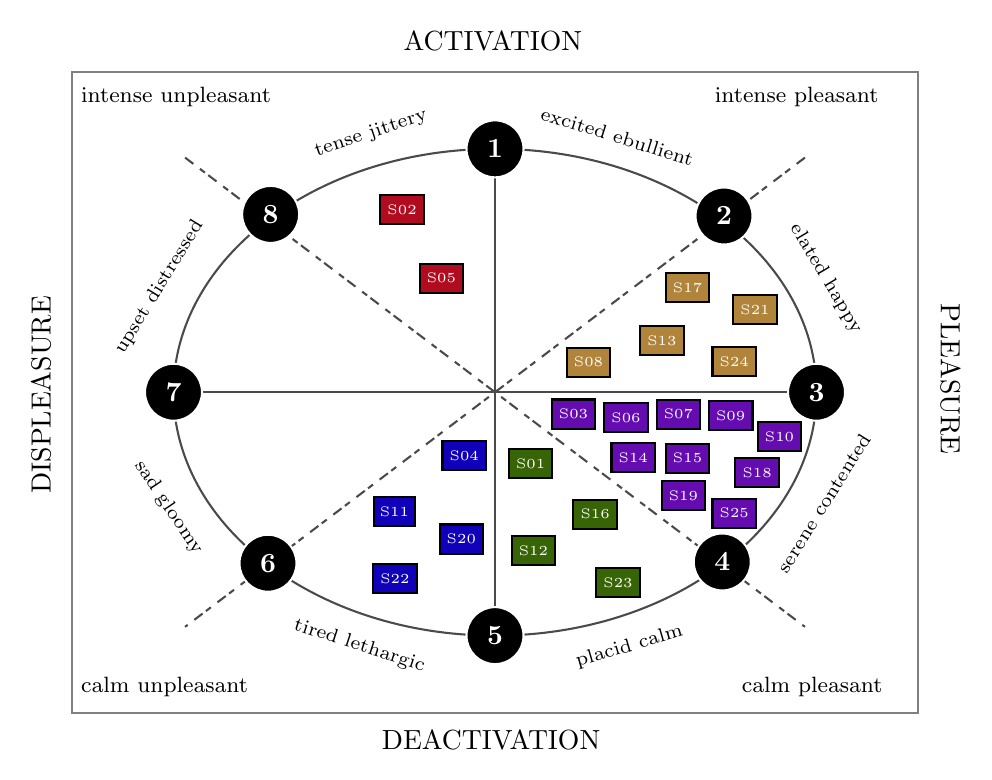
\begin{tikzpicture}[x=0.75pt,y=0.75pt,yscale=-1,xscale=1]
%uncomment if require: \path (0,389); %set diagram left start at 0, and has height of 389

%Flowchart: Or [id:dp3592995680476845] 
\draw  [color={rgb, 255:red, 74; green, 74; blue, 74 }  ,draw opacity=1 ] (182.64,181.1) .. controls (182.64,116.34) and (252,63.84) .. (337.55,63.84) .. controls (423.11,63.84) and (492.46,116.34) .. (492.46,181.1) .. controls (492.46,245.86) and (423.11,298.36) .. (337.55,298.36) .. controls (252,298.36) and (182.64,245.86) .. (182.64,181.1) -- cycle ; \draw  [color={rgb, 255:red, 74; green, 74; blue, 74 }  ,draw opacity=1 ] (182.64,181.1) -- (492.46,181.1) ; \draw  [color={rgb, 255:red, 74; green, 74; blue, 74 }  ,draw opacity=1 ] (337.55,63.84) -- (337.55,298.36) ;
%Straight Lines [id:da30798451784186187] 
\draw [color={rgb, 255:red, 74; green, 74; blue, 74 }  ,draw opacity=1 ] [dash pattern={on 3.75pt off 3pt on 2.25pt off 1.5pt}]  (188.22,68.06) -- (486.88,294.14) ;
%Straight Lines [id:da7804870395610348] 
\draw [color={rgb, 255:red, 74; green, 74; blue, 74 }  ,draw opacity=1 ] [dash pattern={on 3.75pt off 3pt on 2.25pt off 1.5pt}]  (486.88,68.06) -- (188.22,294.14) ;
%Shape: Rectangle [id:dp23344423808181314] 
\draw  [color={rgb, 255:red, 128; green, 128; blue, 128 }  ,draw opacity=1 ] (133.68,26.77) -- (541.42,26.77) -- (541.42,335.43) -- (133.68,335.43) -- cycle ;

% Text Node
\draw  [color={rgb, 255:red, 0; green, 0; blue, 0 }  ,draw opacity=1 ][fill={rgb, 255:red, 176; green, 11; blue, 31 }  ,fill opacity=1 ]  (282.29,86.22) -- (303.29,86.22) -- (303.29,100.22) -- (282.29,100.22) -- cycle  ;
\draw (292.79,93.22) node  [font=\tiny,color={rgb, 255:red, 255; green, 255; blue, 255 }  ,opacity=1 ] [align=left] {S02};
% Text Node
\draw  [color={rgb, 255:red, 0; green, 0; blue, 0 }  ,draw opacity=1 ][fill={rgb, 255:red, 17; green, 0; blue, 185 }  ,fill opacity=1 ]  (279.09,231.64) -- (299.09,231.64) -- (299.09,245.64) -- (279.09,245.64) -- cycle  ;
\draw (289.09,238.64) node  [font=\tiny,color={rgb, 255:red, 255; green, 255; blue, 255 }  ,opacity=1 ] [align=left] {S11};
% Text Node
\draw  [color={rgb, 255:red, 0; green, 0; blue, 0 }  ,draw opacity=1 ][fill={rgb, 255:red, 100; green, 12; blue, 176 }  ,fill opacity=1 ]  (364.87,184.61) -- (385.87,184.61) -- (385.87,198.61) -- (364.87,198.61) -- cycle  ;
\draw (375.37,191.61) node  [font=\tiny,color={rgb, 255:red, 255; green, 255; blue, 255 }  ,opacity=1 ] [align=left] {S03};
% Text Node
\draw  [color={rgb, 255:red, 0; green, 0; blue, 0 }  ,draw opacity=1 ][fill={rgb, 255:red, 176; green, 132; blue, 58 }  ,fill opacity=1 ]  (407.45,149.33) -- (428.45,149.33) -- (428.45,163.33) -- (407.45,163.33) -- cycle  ;
\draw (417.95,156.33) node  [font=\tiny,color={rgb, 255:red, 255; green, 255; blue, 255 }  ,opacity=1 ] [align=left] {S13};
% Text Node
\draw  [color={rgb, 255:red, 0; green, 0; blue, 0 }  ,draw opacity=1 ][fill={rgb, 255:red, 100; green, 12; blue, 176 }  ,fill opacity=1 ]  (440.62,185.49) -- (461.62,185.49) -- (461.62,199.49) -- (440.62,199.49) -- cycle  ;
\draw (451.12,192.49) node  [font=\tiny,color={rgb, 255:red, 255; green, 255; blue, 255 }  ,opacity=1 ] [align=left] {S09};
% Text Node
\draw  [color={rgb, 255:red, 0; green, 0; blue, 0 }  ,draw opacity=1 ][fill={rgb, 255:red, 55; green, 100; blue, 4 }  ,fill opacity=1 ]  (344.22,208.42) -- (365.22,208.42) -- (365.22,222.42) -- (344.22,222.42) -- cycle  ;
\draw (354.72,215.42) node  [font=\tiny,color={rgb, 255:red, 255; green, 255; blue, 255 }  ,opacity=1 ] [align=left] {S01};
% Text Node
\draw  [color={rgb, 255:red, 0; green, 0; blue, 0 }  ,draw opacity=1 ][fill={rgb, 255:red, 176; green, 11; blue, 31 }  ,fill opacity=1 ]  (301.25,119.14) -- (322.25,119.14) -- (322.25,133.14) -- (301.25,133.14) -- cycle  ;
\draw (311.75,126.14) node  [font=\tiny,color={rgb, 255:red, 255; green, 255; blue, 255 }  ,opacity=1 ] [align=left] {S05};
% Text Node
\draw  [color={rgb, 255:red, 0; green, 0; blue, 0 }  ,draw opacity=1 ][fill={rgb, 255:red, 17; green, 0; blue, 185 }  ,fill opacity=1 ]  (312.26,204.61) -- (333.26,204.61) -- (333.26,218.61) -- (312.26,218.61) -- cycle  ;
\draw (322.76,211.61) node  [font=\tiny,color={rgb, 255:red, 255; green, 255; blue, 255 }  ,opacity=1 ] [align=left] {S04};
% Text Node
\draw  [color={rgb, 255:red, 0; green, 0; blue, 0 }  ,draw opacity=1 ][fill={rgb, 255:red, 100; green, 12; blue, 176 }  ,fill opacity=1 ]  (419.83,205.83) -- (440.83,205.83) -- (440.83,219.83) -- (419.83,219.83) -- cycle  ;
\draw (430.33,212.83) node  [font=\tiny,color={rgb, 255:red, 255; green, 255; blue, 255 }  ,opacity=1 ] [align=left] {S15};
% Text Node
\draw  [color={rgb, 255:red, 0; green, 0; blue, 0 }  ,draw opacity=1 ][fill={rgb, 255:red, 100; green, 12; blue, 176 }  ,fill opacity=1 ]  (390.18,186.39) -- (411.18,186.39) -- (411.18,200.39) -- (390.18,200.39) -- cycle  ;
\draw (400.68,193.39) node  [font=\tiny,color={rgb, 255:red, 255; green, 255; blue, 255 }  ,opacity=1 ] [align=left] {S06};
% Text Node
\draw  [color={rgb, 255:red, 0; green, 0; blue, 0 }  ,draw opacity=1 ][fill={rgb, 255:red, 176; green, 132; blue, 58 }  ,fill opacity=1 ]  (372.1,159.61) -- (393.1,159.61) -- (393.1,173.61) -- (372.1,173.61) -- cycle  ;
\draw (382.6,166.61) node  [font=\tiny,color={rgb, 255:red, 255; green, 255; blue, 255 }  ,opacity=1 ] [align=left] {S08};
% Text Node
\draw  [color={rgb, 255:red, 0; green, 0; blue, 0 }  ,draw opacity=1 ][fill={rgb, 255:red, 100; green, 12; blue, 176 }  ,fill opacity=1 ]  (464.11,195.49) -- (485.11,195.49) -- (485.11,209.49) -- (464.11,209.49) -- cycle  ;
\draw (474.61,202.49) node  [font=\tiny,color={rgb, 255:red, 255; green, 255; blue, 255 }  ,opacity=1 ] [align=left] {S10};
% Text Node
\draw  [color={rgb, 255:red, 0; green, 0; blue, 0 }  ,draw opacity=1 ][fill={rgb, 255:red, 100; green, 12; blue, 176 }  ,fill opacity=1 ]  (393.68,205.71) -- (414.68,205.71) -- (414.68,219.71) -- (393.68,219.71) -- cycle  ;
\draw (404.18,212.71) node  [font=\tiny,color={rgb, 255:red, 255; green, 255; blue, 255 }  ,opacity=1 ] [align=left] {S14};
% Text Node
\draw  [color={rgb, 255:red, 0; green, 0; blue, 0 }  ,draw opacity=1 ][fill={rgb, 255:red, 55; green, 100; blue, 4 }  ,fill opacity=1 ]  (345.53,250.28) -- (366.53,250.28) -- (366.53,264.28) -- (345.53,264.28) -- cycle  ;
\draw (356.03,257.28) node  [font=\tiny,color={rgb, 255:red, 255; green, 255; blue, 255 }  ,opacity=1 ] [align=left] {S12};
% Text Node
\draw  [color={rgb, 255:red, 0; green, 0; blue, 0 }  ,draw opacity=1 ][fill={rgb, 255:red, 100; green, 12; blue, 176 }  ,fill opacity=1 ]  (415.44,184.66) -- (436.44,184.66) -- (436.44,198.66) -- (415.44,198.66) -- cycle  ;
\draw (425.94,191.66) node  [font=\tiny,color={rgb, 255:red, 255; green, 255; blue, 255 }  ,opacity=1 ] [align=left] {S07};
% Text Node
\draw  [color={rgb, 255:red, 255; green, 255; blue, 255 }  ,draw opacity=1 ][fill={rgb, 255:red, 0; green, 0; blue, 0 }  ,fill opacity=1 ]  (337.55, 63.84) circle [x radius= 13.73, y radius= 13.73]   ;
\draw (337.55,63.84) node  [font=\normalsize,color={rgb, 255:red, 255; green, 255; blue, 255 }  ,opacity=1 ] [align=left] {\textbf{1}};
% Text Node
\draw  [color={rgb, 255:red, 255; green, 255; blue, 255 }  ,draw opacity=1 ][fill={rgb, 255:red, 0; green, 0; blue, 0 }  ,fill opacity=1 ]  (447.88, 96.18) circle [x radius= 13.73, y radius= 13.73]   ;
\draw (447.88,96.18) node  [font=\normalsize,color={rgb, 255:red, 255; green, 255; blue, 255 }  ,opacity=1 ] [align=left] {\textbf{2}};
% Text Node
\draw  [color={rgb, 255:red, 255; green, 255; blue, 255 }  ,draw opacity=1 ][fill={rgb, 255:red, 0; green, 0; blue, 0 }  ,fill opacity=1 ]  (492.46, 181.1) circle [x radius= 13.73, y radius= 13.73]   ;
\draw (492.46,181.1) node  [font=\normalsize,color={rgb, 255:red, 255; green, 255; blue, 255 }  ,opacity=1 ] [align=left] {\textbf{3}};
% Text Node
\draw  [color={rgb, 255:red, 255; green, 255; blue, 255 }  ,draw opacity=1 ][fill={rgb, 255:red, 0; green, 0; blue, 0 }  ,fill opacity=1 ]  (447.05, 262.88) circle [x radius= 13.73, y radius= 13.73]   ;
\draw (447.05,262.88) node  [font=\normalsize,color={rgb, 255:red, 255; green, 255; blue, 255 }  ,opacity=1 ] [align=left] {\textbf{4}};
% Text Node
\draw  [color={rgb, 255:red, 255; green, 255; blue, 255 }  ,draw opacity=1 ][fill={rgb, 255:red, 0; green, 0; blue, 0 }  ,fill opacity=1 ]  (337.55, 298.36) circle [x radius= 13.73, y radius= 13.73]   ;
\draw (337.55,298.36) node  [font=\normalsize,color={rgb, 255:red, 255; green, 255; blue, 255 }  ,opacity=1 ] [align=left] {\textbf{5}};
% Text Node
\draw  [color={rgb, 255:red, 255; green, 255; blue, 255 }  ,draw opacity=1 ][fill={rgb, 255:red, 0; green, 0; blue, 0 }  ,fill opacity=1 ]  (228.16, 263.49) circle [x radius= 13.73, y radius= 13.73]   ;
\draw (228.16,263.49) node  [font=\normalsize,color={rgb, 255:red, 255; green, 255; blue, 255 }  ,opacity=1 ] [align=left] {\textbf{6}};
% Text Node
\draw  [color={rgb, 255:red, 255; green, 255; blue, 255 }  ,draw opacity=1 ][fill={rgb, 255:red, 0; green, 0; blue, 0 }  ,fill opacity=1 ]  (182.64, 181.1) circle [x radius= 13.73, y radius= 13.73]   ;
\draw (182.64,181.1) node  [font=\normalsize,color={rgb, 255:red, 255; green, 255; blue, 255 }  ,opacity=1 ] [align=left] {\textbf{7}};
% Text Node
\draw  [color={rgb, 255:red, 255; green, 255; blue, 255 }  ,draw opacity=1 ][fill={rgb, 255:red, 0; green, 0; blue, 0 }  ,fill opacity=1 ]  (229.45, 95.43) circle [x radius= 13.73, y radius= 13.73]   ;
\draw (229.45,95.43) node  [font=\normalsize,color={rgb, 255:red, 255; green, 255; blue, 255 }  ,opacity=1 ] [align=left] {\textbf{8}};
% Text Node
\draw (112.89,231.39) node [anchor=north west][inner sep=0.75pt]  [rotate=-270] [align=left] {DISPLEASURE};
% Text Node
\draw (292.08,5.96) node [anchor=north west][inner sep=0.75pt]   [align=left] {ACTIVATION};
% Text Node
\draw (281.58,342.71) node [anchor=north west][inner sep=0.75pt]   [align=left] {DEACTIVATION};
% Text Node
\draw (562.94,136.89) node [anchor=north west][inner sep=0.75pt]  [rotate=-90] [align=left] {PLEASURE};
% Text Node
\draw (150.9,160.23) node [anchor=north west][inner sep=0.75pt]  [font=\scriptsize,rotate=-301.49] [align=left] {upset distressed};
% Text Node
\draw (247.79,60.45) node [anchor=north west][inner sep=0.75pt]  [font=\scriptsize,rotate=-341.6] [align=left] {tense jittery};
% Text Node
\draw (359.94,41.46) node [anchor=north west][inner sep=0.75pt]  [font=\scriptsize,rotate=-17.34] [align=left] {excited ebullient};
% Text Node
\draw (485.75,96.5) node [anchor=north west][inner sep=0.75pt]  [font=\scriptsize,rotate=-59.2] [align=left] {elated happy};
% Text Node
\draw (470.66,265.95) node [anchor=north west][inner sep=0.75pt]  [font=\scriptsize,rotate=-301.93] [align=left] {serene contented};
% Text Node
\draw (373.68,306.2) node [anchor=north west][inner sep=0.75pt]  [font=\scriptsize,rotate=-343.65] [align=left] {placid calm};
% Text Node
\draw (241.21,287.33) node [anchor=north west][inner sep=0.75pt]  [font=\scriptsize,rotate=-18.04] [align=left] {tired lethargic};
% Text Node
\draw (169.56,210.51) node [anchor=north west][inner sep=0.75pt]  [font=\scriptsize,rotate=-56.13] [align=left] {sad gloomy};
% Text Node
\draw (455,317) node [anchor=north west][inner sep=0.75pt]  [font=\footnotesize] [align=left] {calm pleasant};
% Text Node
\draw (136.67,317) node [anchor=north west][inner sep=0.75pt]  [font=\footnotesize] [align=left] {calm unpleasant};
% Text Node
\draw (136.67,32.78) node [anchor=north west][inner sep=0.75pt]  [font=\footnotesize] [align=left] {intense unpleasant};
% Text Node
\draw (442,32.78) node [anchor=north west][inner sep=0.75pt]  [font=\footnotesize] [align=left] {intense pleasant};
% Text Node
\draw  [color={rgb, 255:red, 0; green, 0; blue, 0 }  ,draw opacity=1 ][fill={rgb, 255:red, 55; green, 100; blue, 4 }  ,fill opacity=1 ]  (375.33,232.83) -- (396.33,232.83) -- (396.33,246.83) -- (375.33,246.83) -- cycle  ;
\draw (385.83,239.83) node  [font=\tiny,color={rgb, 255:red, 255; green, 255; blue, 255 }  ,opacity=1 ] [align=left] {S16};
% Text Node
\draw  [color={rgb, 255:red, 0; green, 0; blue, 0 }  ,draw opacity=1 ][fill={rgb, 255:red, 176; green, 132; blue, 58 }  ,fill opacity=1 ]  (419.83,123.83) -- (440.83,123.83) -- (440.83,137.83) -- (419.83,137.83) -- cycle  ;
\draw (430.33,130.83) node  [font=\tiny,color={rgb, 255:red, 255; green, 255; blue, 255 }  ,opacity=1 ] [align=left] {S17};
% Text Node
\draw  [color={rgb, 255:red, 0; green, 0; blue, 0 }  ,draw opacity=1 ][fill={rgb, 255:red, 100; green, 12; blue, 176 }  ,fill opacity=1 ]  (453.33,212.83) -- (474.33,212.83) -- (474.33,226.83) -- (453.33,226.83) -- cycle  ;
\draw (463.83,219.83) node  [font=\tiny,color={rgb, 255:red, 255; green, 255; blue, 255 }  ,opacity=1 ] [align=left] {S18};
% Text Node
\draw  [color={rgb, 255:red, 0; green, 0; blue, 0 }  ,draw opacity=1 ][fill={rgb, 255:red, 100; green, 12; blue, 176 }  ,fill opacity=1 ]  (417.83,223.83) -- (438.83,223.83) -- (438.83,237.83) -- (417.83,237.83) -- cycle  ;
\draw (428.33,230.83) node  [font=\tiny,color={rgb, 255:red, 255; green, 255; blue, 255 }  ,opacity=1 ] [align=left] {S19};
% Text Node
\draw  [color={rgb, 255:red, 0; green, 0; blue, 0 }  ,draw opacity=1 ][fill={rgb, 255:red, 17; green, 0; blue, 185 }  ,fill opacity=1 ]  (310.83,244.83) -- (331.83,244.83) -- (331.83,258.83) -- (310.83,258.83) -- cycle  ;
\draw (321.33,251.83) node  [font=\tiny,color={rgb, 255:red, 255; green, 255; blue, 255 }  ,opacity=1 ] [align=left] {S20};
% Text Node
\draw  [color={rgb, 255:red, 0; green, 0; blue, 0 }  ,draw opacity=1 ][fill={rgb, 255:red, 176; green, 132; blue, 58 }  ,fill opacity=1 ]  (452.33,134.33) -- (473.33,134.33) -- (473.33,148.33) -- (452.33,148.33) -- cycle  ;
\draw (462.83,141.33) node  [font=\tiny,color={rgb, 255:red, 255; green, 255; blue, 255 }  ,opacity=1 ] [align=left] {S21};
% Text Node
\draw  [color={rgb, 255:red, 0; green, 0; blue, 0 }  ,draw opacity=1 ][fill={rgb, 255:red, 17; green, 0; blue, 185 }  ,fill opacity=1 ]  (278.83,263.83) -- (299.83,263.83) -- (299.83,277.83) -- (278.83,277.83) -- cycle  ;
\draw (289.33,270.83) node  [font=\tiny,color={rgb, 255:red, 255; green, 255; blue, 255 }  ,opacity=1 ] [align=left] {S22};
% Text Node
\draw  [color={rgb, 255:red, 0; green, 0; blue, 0 }  ,draw opacity=1 ][fill={rgb, 255:red, 55; green, 100; blue, 4 }  ,fill opacity=1 ]  (386.33,265.83) -- (407.33,265.83) -- (407.33,279.83) -- (386.33,279.83) -- cycle  ;
\draw (396.83,272.83) node  [font=\tiny,color={rgb, 255:red, 255; green, 255; blue, 255 }  ,opacity=1 ] [align=left] {S23};
% Text Node
\draw  [color={rgb, 255:red, 0; green, 0; blue, 0 }  ,draw opacity=1 ][fill={rgb, 255:red, 176; green, 132; blue, 58 }  ,fill opacity=1 ]  (442.33,159.33) -- (463.33,159.33) -- (463.33,173.33) -- (442.33,173.33) -- cycle  ;
\draw (452.83,166.33) node  [font=\tiny,color={rgb, 255:red, 255; green, 255; blue, 255 }  ,opacity=1 ] [align=left] {S24};
% Text Node
\draw  [color={rgb, 255:red, 0; green, 0; blue, 0 }  ,draw opacity=1 ][fill={rgb, 255:red, 100; green, 12; blue, 176 }  ,fill opacity=1 ]  (442.33,232.33) -- (463.33,232.33) -- (463.33,246.33) -- (442.33,246.33) -- cycle  ;
\draw (452.83,239.33) node  [font=\tiny,color={rgb, 255:red, 255; green, 255; blue, 255 }  ,opacity=1 ] [align=left] {S25};


\end{tikzpicture}

    \fonte{Author.}
\end{figure}

% Levando em consideração que são abordagens que em sua essência são diametralmente opostas, acreditamos que a similaridade dos resultados observados pode ser um bom sinal.
% Isso indica em um primeiro momento que nossa proposta alcança um nível similar de satisfação, semelhante ao de outra ferramenta já madura e amplamente estabelecida.
% Contudo, para verificarmos mais a fundo isto foi então feito um terceiro experimento visando avaliar os geradores implementados, de uma forma mais qualitativa, uma vez que já possuímos material estatísticamente relevante e que suporta nossas conclusões em relação as hipóteses tratadas.
Seeing that these are approaches that, in essence, are opposed, we believe that the similarity of the observed results may be a good sign.
%Taking into account that these are approaches that, in essence, are diametrically opposed, we believe that the similarity of the observed results may be a good sign.
Firstly, this indicates that our proposal achieves a similar level of satisfaction as the other mature and widely established tool.
%This indicates at first that our proposal achieves a similar level of satisfaction, similar to that of another mature and widely established tool.
However, further to check this better, we carried out a third experiment to evaluate the implemented generators, this time qualitatively, since we already have the statistically relevant material that supports our conclusions concerning the hypotheses treated.
%However, to further verify this, a third experiment was carried out to evaluate the implemented generators, in a more qualitative way, since we already have statistically relevant material that supports our conclusions in relation to the hypotheses treated.

%######################################################
\subsection{Experiment 3}
\label{ssec_experiments:Experiment3}
%######################################################

% O \ac{ex3} foi realizado na segunda metade de fevereiro de 2022.
% Os vinte e cinto (25) participantes do \ac{ex2} foram novamente convidados a participarem.
% Houve a aceitação de quinze (15) sujeitos.
We carried out \ac{ex3} in the second half of February 2022.
% \ac{ex3} was carried out in the second half of February 2022.
We again invited twenty-five (25) participants from \ac{ex2} to participate.
% The twenty-five (25) participants of \ac{ex2} were again invited to participate.
There were the acceptance of fifteen (15) subjects.
% There was the acceptance of fifteen (15) subjects.

% Desta vez o protocolo original foi novamente modificado.
% Nesta execução não procuramos realizar a medição do tempo ou da qualidade dos modelos produzidos.
% Da mesma maneira, os participantes precisavam realizar a modelagem de dois (2) problemas simples, um com cada abordagem.
This time, we modified the original protocol again.
% This time the original protocol was modified again.
In this execution, we do not seek to measure the time or quality of the models produced.
Likewise, we required the participants to model two (2) simple problems, one with each approach.
% Likewise, participants were required to model two (2) simple problems, one with each approach.

% O ambiente controlado deixou de ser uma máquina virtual, uma vez que houve a geração de um plugin completo para o Eclipse e disponibilizado publicamente .
% Este plugin tinha como dependência de funcionamento apenas a instalação de uma IDE Eclipse e do Java, independentemente do sistema operacional usado.
% De toda a forma as atividades ocorreram de forma remota, quando como nos outros experimentos os pesquisadores acompanharam de maneira online os sujeitos.
The controlled environment was no longer in a virtual machine since a complete plugin for Eclipse was generated and made publicly available.
This plugin only depended on the Eclipse IDE and Java installation, regardless of the operating system utilized.
%This plugin only depended on the installation of an Eclipse IDE and Java, regardless of the operating system used.
In any case, the activities took place remotely when as in the other experiments, the researchers followed the subjects online.

% Os instrumentos também foram diferentes, já que nesta execução os instrumentos de avaliação dos contrutores e atributos de qualidade foram omitidos.
% Nossa intenção era que os sujeitos avaliassem os artefatos gerados pelas ferramentas que suportavam as abordagens, nos diferentes níveis suportados.
% Para isto utilizou-se uma escala Likert para se obter a avaliação destes artefatos gerados em cada um dos níveis de modelagem (conceitual, lógico e físico).
The instruments were also different in this execution since we omitted the builders' assessment instruments and the quality attributes.
% The instruments were also different, since in this execution the builders' assessment instruments and quality attributes were omitted.
Our intention was for the subjects to evaluate the artifacts generated by the tools that supported the approaches at the different levels.
For this, we used a Likert~\cite{Likert} scale to obtain the evaluation of these artifacts generated in each of the modeling levels (conceptual, logical, and physical).
% For this, a Likert scale was used to obtain the evaluation of these artifacts generated in each of the modeling levels (conceptual, logical and physical).

% Foi ainda reutilizado o método Emocards descrito anteriormente, visando entender o estado de espírito que o uso das ferramentas por completo podiam causar.
% Nós também adicionamos uma série de perguntas abertas e, finalmente, um formulário com uma conhecida escala de usabilidade utilizada na engenharia de sistemas, nomeada \ac{sus}~\cite{sus:1995}.
The Emocards method described previously was also reused to understand the state of mind that utilization of the full features in the tools could cause.
%The Emocards method described previously was also reused, in order to understand the state of mind that the use of fully features in the tools could cause.
Beyond, we also added a series of open-ended questions and, finally, a form with a well-known usability scale utilized in systems engineering named \ac{sus}~\cite{sus:1995}.
%We also added a series of open-ended questions and, finally, a form with a well-known usability scale used in systems engineering, named \ac{sus}~\cite{sus:1995}.
 
%###########################################################
\subsubsection{Results Analysis}
%###########################################################

% No que diz respeito a avaliação dos artefatos relacionados aos níveis de modelagem, a Figura \ref{fig:ToolModelsEval} apresenta o resumo dos valores obtidos.
% Em relação a classificação os modelos conceituais produzidos, houve uma melhor aceitação por parte da abordagem gráfica, na ferramenta brModelo.
% Foram onze (11) avaliações com conceito máximo, em contraste a abordagem textual, utilizando a solução proposta ERtext.
% A abordagem textual, além de ter menos avaliações máximas, totalizando sete (7), ainda teve avaliações com score dois (2), ou seja, baixas.
% Para deixar registrado, a escala Likert usada ia de um (1 - a pior avaliação) até seis (6 - a melhor avaliação), e enquanto o modelo conceitual da abordagem gráfica era apenas o diagrama, a abordagem textual era representado pelo modelo escrito e acompanhado de um equivalente gráfico que utilizava elementos \ac{uml}.
Regarding the artifacts evaluation related to the modeling levels, Figure \ref{fig:ToolModelsEval}  presents a brief of the values obtained.
%Regarding the evaluation of artifacts related to the modeling levels, Figure \ref{fig:ToolModelsEval} presents a summary of the values obtained.
Concerning the classification of the conceptual models produced, there was a better acceptance of the graphical approach in the brModelo tool.
In contrast to the textual approach, the proposed ERtext solution received eleven (11) evaluations with a maximum score.
% There were eleven (11) evaluations with maximum concept, in contrast to the textual approach, using the proposed ERtext solution.
In addition to having fewer maximum scores, the textual approach, which totaled seven (7), still had evaluations with a score of two (2), \textit{i.e.}, low considerations.
% The textual approach, in addition to having fewer maximum ratings, totaling seven (7), still had ratings with a score of two (2), that is, low considerations.
We applied the Likert~\cite{Likert} scale ranging from one (1 - the worst rating) to six (6 - the best rating). It is worth noting that while the conceptual model of the graphical approach was just the diagram, the textual one has represented by the textual model and accompanied by a graphic equivalent that used UML elements.
% For the record, the Likert scale used ranged from one (1 - the worst rating) to six (6 - the best rating), and while the conceptual model of the graphical approach was just the diagram, the textual approach was represented by the textual model and accompanied by a graphical equivalent that used \ac{uml} elements.

\begin{figure}[!htb]
    \centering
    \caption{Evaluation of produced artifacts per treatments.}
    \label{fig:ToolModelsEval}
    \pgfplotsset{testbar/.style={
        xbar stacked,
        legend cell align=left,
        legend style={
            legend columns=8,
            font=\scriptsize,
            at={(xticklabel cs:1.0)},
            anchor=north east,
            draw=none,
            nodes={scale=1}
            },
        width=10cm,
        axis y line*= none, 
        axis x line*= bottom,
        xmajorgrids = false,
        xmin=0,xmax=15,
        ytick = data,
        yticklabels = {
            {\scriptsize Conceptual Model-ERtext},
            {\scriptsize Conceptual Model-brModelo},
            {\scriptsize Logical Model-ERtext},
            {\scriptsize Logical Model-brModelo},
            {\scriptsize Physical Model-ERtext},
            {\scriptsize Physical Model-brModelo}
        },
        tick align = outside, 
        xtick pos = left,
        xticklabel style = {font=\scriptsize},
        bar width=5mm, 
        y=7mm,
        enlarge y limits={abs=0.450},% 0.5 + 0.5*(y - bar width)/y [TeX.sx #47995]
        nodes near coords,
        nodes near coords align=center,%Move values in bar
        every node near coord/.append style={
            black,
            font=\scriptsize,
            text opacity=1,
            fill=white,
            fill opacity=0.5,
            outer sep=\pgflinewidth
        }
    }}
    \begin{tikzpicture}
    \begin{axis}[testbar] 
    \addplot[pattern color=red,pattern=north east lines] coordinates
        {(0,6)(0,5)(0,4)(0,3)(0,2)(0,1)};
    \addplot[pattern color=teal,pattern=vertical lines] coordinates
        {(0,6)(0,5)(0,4)(0,3)(0,2)(0,1)};
    \addplot[pattern color=gray, pattern=grid] coordinates
        {(2,6)(0,5)(2,4)(2,3)(0,2)(3,1)};
    \addplot[pattern color=magenta, pattern=north west lines] coordinates
        {(1,6)(0,5)(2,4)(1,3)(3,2)(3,1)};
    \addplot[pattern color=blue, pattern=horizontal lines] coordinates
        {(5,6)(4,5)(4,4)(7,3)(3,2)(4,1)};
    \addplot[pattern color=green, pattern=crosshatch dots] coordinates
        {(7,6)(11,5)(7,4)(5,3)(9,2)(5,1)};
    \legend{1-Strongly Bad, 2, 3, 4, 5, 6-Strongly Good}
    \end{axis}
    \end{tikzpicture}
    \fonte{Author.}
\end{figure}

% Quanto a avaliação dos modelos lógicos gerados a partir dos modelos conceituais, houve uma equivalência maior, mas com uma pequena vantagem para a abordagem textual.
% Em relação a avaliação dos modelos físicos, foi pedido que os códigos \ac{sql} fossem executados em um \ac{dbms}, especificamente o PostgreSQL uma vez que o mesmo era utilizado de forma recorrente na classe de projeto e modelagem de banco de dados.
Respecting the evaluation of the logical models generated from the conceptual models, we recognize the most equivalency but with fewer advantages for the textual approach.
%Regarding the evaluation of the logical models generated from the conceptual models, there was a greater equivalence, but with a small advantage for the textual approach.
Regarding the evaluation of the physical models, we requested that the subjects run the \ac{sql} codes generated in a \ac{dbms}, specifically PostgreSQL since it has been used recurrently in the Databases' classes.
%Regarding the evaluation of the physical models, it was requested that the \ac{sql} codes were executed in a \ac{dbms}, specifically PostgreSQL, since it was used in a recurrent way in the classes.

% Os resultados dos modelos físicos mostraram uma vantagem leve para a abordagem textual, tendo ainda abordagem gráfica recebido avaliações com score (2), ou seja, considerando os modelos com qualidade baixa.
The results of the physical models showed a slight advantage for the textual approach, and the graphical one also received evaluations with a score (2), that is, considering the models with low quality.

% É importante salientar que a cada avaliação dos artefatos ainda era perguntado, de forma aberta, se existia critícas, elogios, dúvidas ou sugestões de melhoria quanto a representações observadas.
% As respostas coletadas serviriam depois para uma análise qualitativa utilizando codificação qualitativa.
It is relevant to point out that at each evaluation of the artifacts, it was still openly asked if there were criticisms, compliments, doubts, or suggestions for improvement regarding the observed representations.
Then the collected responses would be used for a qualitative analysis using qualitative coding.

% Quanto a avaliação utilizando o método Emocards, os resultados são apresentados nas Figuras \ref{fig:Emocards4_alt} e \ref{fig:Emocards3_alt}.
% Novamente houveram resultados muito aproximados, demonstrando que ambas as ferramentas conseguem despertar sentimentos e estados de espírito similares.
As for the evaluation using the Emocards method, Figures show \ref{fig:Emocards4_alt} and \ref{fig:Emocards3_alt} the results.
Again, there were very similar results, demonstrating that both tools can arouse similar feelings and states of mind.
%Again, there were very similar results, demonstrating that both tools are able to arouse similar feelings and states of mind.

% Nos Emocards relativos a abordagem textual (Figura \ref{fig:Emocards4_alt}), utilizando a ERtext, houve cinco (5) sujeitos que expressaram estarem no quadrante que engloba sentimentos de felicidade.
% Outros nove (9) sujeitos demonstraram estarem no quadrante que envolve sentimentos relacionados a relaxamento, e apenas um (1) participante escolheu uma representação gráfica de face humana que era classificada no quadrante que compreende sentimentos de irritabilidade. 
In the Emocards related to the textual approach (Figure \ref{fig:Emocards4_alt}), using ERtext, we received five (5) responses from subjects who expressed being in the quadrant that encompasses feelings of happiness.
%In the Emocards related to the textual approach (Figure \ref{fig:Emocards4_alt}), using ERtext, there were five (5) subjects who expressed being in the quadrant that encompasses feelings of happiness.
From another point of view, another nine (9) responses from subjects showed being in the quadrant that involves feelings related to relaxation. 
Ending, only one (1) participant chose a graphic representation of the human face classified in the quadrant that comprises feelings of irritability.
%Another nine (9) subjects were shown to be in the quadrant that involves feelings related to relaxation, and only one (1) participant chose a graphic representation of the human face that was classified in the quadrant that comprises feelings of irritability.

\begin{figure}[!htb]
    \centering
    \caption{EX3 Emocards - ERtext.}
    \label{fig:Emocards4_alt}
    

\tikzset{every picture/.style={line width=0.75pt}} %set default line width to 0.75pt        

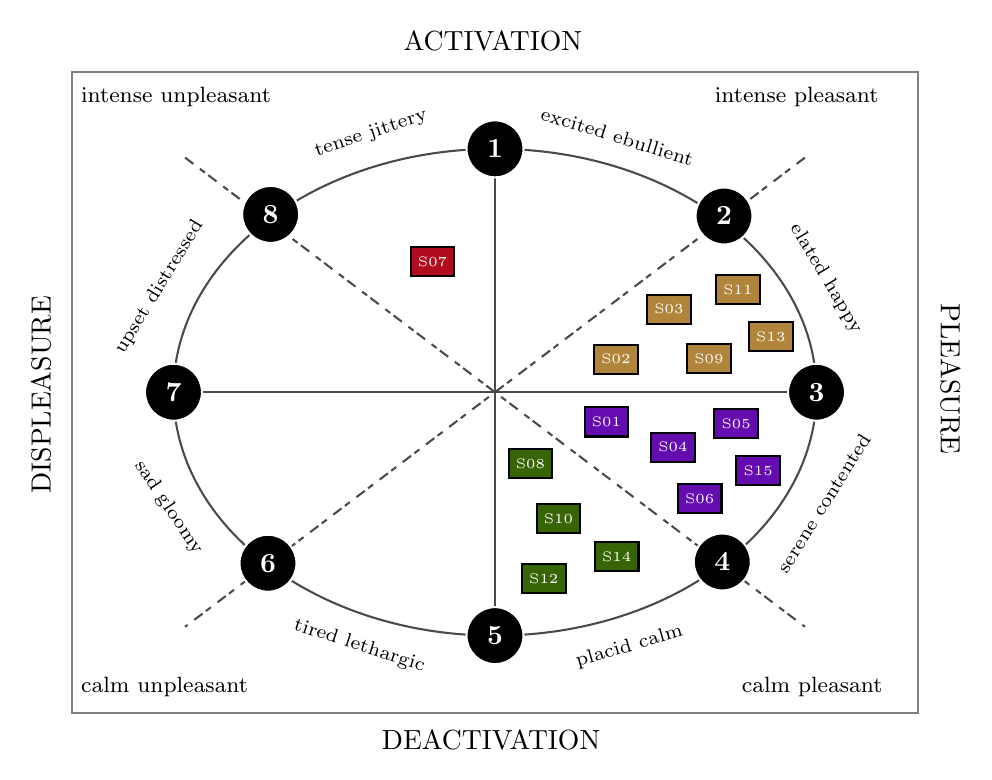
\begin{tikzpicture}[x=0.75pt,y=0.75pt,yscale=-1,xscale=1]
%uncomment if require: \path (0,389); %set diagram left start at 0, and has height of 389

%Flowchart: Or [id:dp3592995680476845] 
\draw  [color={rgb, 255:red, 74; green, 74; blue, 74 }  ,draw opacity=1 ] (182.64,181.1) .. controls (182.64,116.34) and (252,63.84) .. (337.55,63.84) .. controls (423.11,63.84) and (492.46,116.34) .. (492.46,181.1) .. controls (492.46,245.86) and (423.11,298.36) .. (337.55,298.36) .. controls (252,298.36) and (182.64,245.86) .. (182.64,181.1) -- cycle ; \draw  [color={rgb, 255:red, 74; green, 74; blue, 74 }  ,draw opacity=1 ] (182.64,181.1) -- (492.46,181.1) ; \draw  [color={rgb, 255:red, 74; green, 74; blue, 74 }  ,draw opacity=1 ] (337.55,63.84) -- (337.55,298.36) ;
%Straight Lines [id:da30798451784186187] 
\draw [color={rgb, 255:red, 74; green, 74; blue, 74 }  ,draw opacity=1 ] [dash pattern={on 3.75pt off 3pt on 2.25pt off 1.5pt}]  (188.22,68.06) -- (486.88,294.14) ;
%Straight Lines [id:da7804870395610348] 
\draw [color={rgb, 255:red, 74; green, 74; blue, 74 }  ,draw opacity=1 ] [dash pattern={on 3.75pt off 3pt on 2.25pt off 1.5pt}]  (486.88,68.06) -- (188.22,294.14) ;
%Shape: Rectangle [id:dp23344423808181314] 
\draw  [color={rgb, 255:red, 128; green, 128; blue, 128 }  ,draw opacity=1 ] (133.68,26.77) -- (541.42,26.77) -- (541.42,335.43) -- (133.68,335.43) -- cycle ;

% Text Node
\draw  [color={rgb, 255:red, 0; green, 0; blue, 0 }  ,draw opacity=1 ][fill={rgb, 255:red, 176; green, 132; blue, 58 }  ,fill opacity=1 ]  (385.29,158.22) -- (406.29,158.22) -- (406.29,172.22) -- (385.29,172.22) -- cycle  ;
\draw (395.79,165.22) node  [font=\tiny,color={rgb, 255:red, 255; green, 255; blue, 255 }  ,opacity=1 ] [align=left] {S02};
% Text Node
\draw  [color={rgb, 255:red, 0; green, 0; blue, 0 }  ,draw opacity=1 ][fill={rgb, 255:red, 176; green, 132; blue, 58 }  ,fill opacity=1 ]  (444.09,124.64) -- (465.09,124.64) -- (465.09,138.64) -- (444.09,138.64) -- cycle  ;
\draw (454.59,131.64) node  [font=\tiny,color={rgb, 255:red, 255; green, 255; blue, 255 }  ,opacity=1 ] [align=left] {S11};
% Text Node
\draw  [color={rgb, 255:red, 0; green, 0; blue, 0 }  ,draw opacity=1 ][fill={rgb, 255:red, 176; green, 132; blue, 58 }  ,fill opacity=1 ]  (410.87,134.11) -- (431.87,134.11) -- (431.87,148.11) -- (410.87,148.11) -- cycle  ;
\draw (421.37,141.11) node  [font=\tiny,color={rgb, 255:red, 255; green, 255; blue, 255 }  ,opacity=1 ] [align=left] {S03};
% Text Node
\draw  [color={rgb, 255:red, 0; green, 0; blue, 0 }  ,draw opacity=1 ][fill={rgb, 255:red, 176; green, 132; blue, 58 }  ,fill opacity=1 ]  (459.95,147.33) -- (480.95,147.33) -- (480.95,161.33) -- (459.95,161.33) -- cycle  ;
\draw (470.45,154.33) node  [font=\tiny,color={rgb, 255:red, 255; green, 255; blue, 255 }  ,opacity=1 ] [align=left] {S13};
% Text Node
\draw  [color={rgb, 255:red, 0; green, 0; blue, 0 }  ,draw opacity=1 ][fill={rgb, 255:red, 176; green, 132; blue, 58 }  ,fill opacity=1 ]  (430.12,157.99) -- (451.12,157.99) -- (451.12,171.99) -- (430.12,171.99) -- cycle  ;
\draw (440.62,164.99) node  [font=\tiny,color={rgb, 255:red, 255; green, 255; blue, 255 }  ,opacity=1 ] [align=left] {S09};
% Text Node
\draw  [color={rgb, 255:red, 0; green, 0; blue, 0 }  ,draw opacity=1 ][fill={rgb, 255:red, 100; green, 12; blue, 176 }  ,fill opacity=1 ]  (380.72,188.42) -- (401.72,188.42) -- (401.72,202.42) -- (380.72,202.42) -- cycle  ;
\draw (391.22,195.42) node  [font=\tiny,color={rgb, 255:red, 255; green, 255; blue, 255 }  ,opacity=1 ] [align=left] {S01};
% Text Node
\draw  [color={rgb, 255:red, 0; green, 0; blue, 0 }  ,draw opacity=1 ][fill={rgb, 255:red, 100; green, 12; blue, 176 }  ,fill opacity=1 ]  (443.25,189.14) -- (464.25,189.14) -- (464.25,203.14) -- (443.25,203.14) -- cycle  ;
\draw (453.75,196.14) node  [font=\tiny,color={rgb, 255:red, 255; green, 255; blue, 255 }  ,opacity=1 ] [align=left] {S05};
% Text Node
\draw  [color={rgb, 255:red, 0; green, 0; blue, 0 }  ,draw opacity=1 ][fill={rgb, 255:red, 100; green, 12; blue, 176 }  ,fill opacity=1 ]  (412.76,200.61) -- (433.76,200.61) -- (433.76,214.61) -- (412.76,214.61) -- cycle  ;
\draw (423.26,207.61) node  [font=\tiny,color={rgb, 255:red, 255; green, 255; blue, 255 }  ,opacity=1 ] [align=left] {S04};
% Text Node
\draw  [color={rgb, 255:red, 0; green, 0; blue, 0 }  ,draw opacity=1 ][fill={rgb, 255:red, 100; green, 12; blue, 176 }  ,fill opacity=1 ]  (453.83,211.83) -- (474.83,211.83) -- (474.83,225.83) -- (453.83,225.83) -- cycle  ;
\draw (464.33,218.83) node  [font=\tiny,color={rgb, 255:red, 255; green, 255; blue, 255 }  ,opacity=1 ] [align=left] {S15};
% Text Node
\draw  [color={rgb, 255:red, 0; green, 0; blue, 0 }  ,draw opacity=1 ][fill={rgb, 255:red, 100; green, 12; blue, 176 }  ,fill opacity=1 ]  (425.68,225.39) -- (446.68,225.39) -- (446.68,239.39) -- (425.68,239.39) -- cycle  ;
\draw (436.18,232.39) node  [font=\tiny,color={rgb, 255:red, 255; green, 255; blue, 255 }  ,opacity=1 ] [align=left] {S06};
% Text Node
\draw  [color={rgb, 255:red, 0; green, 0; blue, 0 }  ,draw opacity=1 ][fill={rgb, 255:red, 55; green, 100; blue, 4 }  ,fill opacity=1 ]  (344.1,208.52) -- (365.1,208.52) -- (365.1,222.52) -- (344.1,222.52) -- cycle  ;
\draw (354.6,215.52) node  [font=\tiny,color={rgb, 255:red, 255; green, 255; blue, 255 }  ,opacity=1 ] [align=left] {S08};
% Text Node
\draw  [color={rgb, 255:red, 0; green, 0; blue, 0 }  ,draw opacity=1 ][fill={rgb, 255:red, 55; green, 100; blue, 4 }  ,fill opacity=1 ]  (357.61,234.99) -- (378.61,234.99) -- (378.61,248.99) -- (357.61,248.99) -- cycle  ;
\draw (368.11,241.99) node  [font=\tiny,color={rgb, 255:red, 255; green, 255; blue, 255 }  ,opacity=1 ] [align=left] {S10};
% Text Node
\draw  [color={rgb, 255:red, 0; green, 0; blue, 0 }  ,draw opacity=1 ][fill={rgb, 255:red, 55; green, 100; blue, 4 }  ,fill opacity=1 ]  (385.68,253.21) -- (406.68,253.21) -- (406.68,267.21) -- (385.68,267.21) -- cycle  ;
\draw (396.18,260.21) node  [font=\tiny,color={rgb, 255:red, 255; green, 255; blue, 255 }  ,opacity=1 ] [align=left] {S14};
% Text Node
\draw  [color={rgb, 255:red, 0; green, 0; blue, 0 }  ,draw opacity=1 ][fill={rgb, 255:red, 55; green, 100; blue, 4 }  ,fill opacity=1 ]  (350.53,263.78) -- (371.53,263.78) -- (371.53,277.78) -- (350.53,277.78) -- cycle  ;
\draw (361.03,270.78) node  [font=\tiny,color={rgb, 255:red, 255; green, 255; blue, 255 }  ,opacity=1 ] [align=left] {S12};
% Text Node
\draw  [color={rgb, 255:red, 0; green, 0; blue, 0 }  ,draw opacity=1 ][fill={rgb, 255:red, 176; green, 11; blue, 31 }  ,fill opacity=1 ]  (296.94,111.16) -- (317.94,111.16) -- (317.94,125.16) -- (296.94,125.16) -- cycle  ;
\draw (307.44,118.16) node  [font=\tiny,color={rgb, 255:red, 255; green, 255; blue, 255 }  ,opacity=1 ] [align=left] {S07};
% Text Node
\draw  [color={rgb, 255:red, 255; green, 255; blue, 255 }  ,draw opacity=1 ][fill={rgb, 255:red, 0; green, 0; blue, 0 }  ,fill opacity=1 ]  (337.55, 63.84) circle [x radius= 13.73, y radius= 13.73]   ;
\draw (337.55,63.84) node  [font=\normalsize,color={rgb, 255:red, 255; green, 255; blue, 255 }  ,opacity=1 ] [align=left] {\textbf{1}};
% Text Node
\draw  [color={rgb, 255:red, 255; green, 255; blue, 255 }  ,draw opacity=1 ][fill={rgb, 255:red, 0; green, 0; blue, 0 }  ,fill opacity=1 ]  (447.88, 96.18) circle [x radius= 13.73, y radius= 13.73]   ;
\draw (447.88,96.18) node  [font=\normalsize,color={rgb, 255:red, 255; green, 255; blue, 255 }  ,opacity=1 ] [align=left] {\textbf{2}};
% Text Node
\draw  [color={rgb, 255:red, 255; green, 255; blue, 255 }  ,draw opacity=1 ][fill={rgb, 255:red, 0; green, 0; blue, 0 }  ,fill opacity=1 ]  (492.46, 181.1) circle [x radius= 13.73, y radius= 13.73]   ;
\draw (492.46,181.1) node  [font=\normalsize,color={rgb, 255:red, 255; green, 255; blue, 255 }  ,opacity=1 ] [align=left] {\textbf{3}};
% Text Node
\draw  [color={rgb, 255:red, 255; green, 255; blue, 255 }  ,draw opacity=1 ][fill={rgb, 255:red, 0; green, 0; blue, 0 }  ,fill opacity=1 ]  (447.05, 262.88) circle [x radius= 13.73, y radius= 13.73]   ;
\draw (447.05,262.88) node  [font=\normalsize,color={rgb, 255:red, 255; green, 255; blue, 255 }  ,opacity=1 ] [align=left] {\textbf{4}};
% Text Node
\draw  [color={rgb, 255:red, 255; green, 255; blue, 255 }  ,draw opacity=1 ][fill={rgb, 255:red, 0; green, 0; blue, 0 }  ,fill opacity=1 ]  (337.55, 298.36) circle [x radius= 13.73, y radius= 13.73]   ;
\draw (337.55,298.36) node  [font=\normalsize,color={rgb, 255:red, 255; green, 255; blue, 255 }  ,opacity=1 ] [align=left] {\textbf{5}};
% Text Node
\draw  [color={rgb, 255:red, 255; green, 255; blue, 255 }  ,draw opacity=1 ][fill={rgb, 255:red, 0; green, 0; blue, 0 }  ,fill opacity=1 ]  (228.16, 263.49) circle [x radius= 13.73, y radius= 13.73]   ;
\draw (228.16,263.49) node  [font=\normalsize,color={rgb, 255:red, 255; green, 255; blue, 255 }  ,opacity=1 ] [align=left] {\textbf{6}};
% Text Node
\draw  [color={rgb, 255:red, 255; green, 255; blue, 255 }  ,draw opacity=1 ][fill={rgb, 255:red, 0; green, 0; blue, 0 }  ,fill opacity=1 ]  (182.64, 181.1) circle [x radius= 13.73, y radius= 13.73]   ;
\draw (182.64,181.1) node  [font=\normalsize,color={rgb, 255:red, 255; green, 255; blue, 255 }  ,opacity=1 ] [align=left] {\textbf{7}};
% Text Node
\draw  [color={rgb, 255:red, 255; green, 255; blue, 255 }  ,draw opacity=1 ][fill={rgb, 255:red, 0; green, 0; blue, 0 }  ,fill opacity=1 ]  (229.45, 95.43) circle [x radius= 13.73, y radius= 13.73]   ;
\draw (229.45,95.43) node  [font=\normalsize,color={rgb, 255:red, 255; green, 255; blue, 255 }  ,opacity=1 ] [align=left] {\textbf{8}};
% Text Node
\draw (112.89,231.39) node [anchor=north west][inner sep=0.75pt]  [rotate=-270] [align=left] {DISPLEASURE};
% Text Node
\draw (292.08,5.96) node [anchor=north west][inner sep=0.75pt]   [align=left] {ACTIVATION};
% Text Node
\draw (281.58,342.71) node [anchor=north west][inner sep=0.75pt]   [align=left] {DEACTIVATION};
% Text Node
\draw (562.94,136.89) node [anchor=north west][inner sep=0.75pt]  [rotate=-90] [align=left] {PLEASURE};
% Text Node
\draw (150.9,160.23) node [anchor=north west][inner sep=0.75pt]  [font=\scriptsize,rotate=-301.49] [align=left] {upset distressed};
% Text Node
\draw (247.79,60.45) node [anchor=north west][inner sep=0.75pt]  [font=\scriptsize,rotate=-341.6] [align=left] {tense jittery};
% Text Node
\draw (359.94,41.46) node [anchor=north west][inner sep=0.75pt]  [font=\scriptsize,rotate=-17.34] [align=left] {excited ebullient};
% Text Node
\draw (485.75,96.5) node [anchor=north west][inner sep=0.75pt]  [font=\scriptsize,rotate=-59.2] [align=left] {elated happy};
% Text Node
\draw (470.66,265.95) node [anchor=north west][inner sep=0.75pt]  [font=\scriptsize,rotate=-301.93] [align=left] {serene contented};
% Text Node
\draw (373.68,306.2) node [anchor=north west][inner sep=0.75pt]  [font=\scriptsize,rotate=-343.65] [align=left] {placid calm};
% Text Node
\draw (241.21,287.33) node [anchor=north west][inner sep=0.75pt]  [font=\scriptsize,rotate=-18.04] [align=left] {tired lethargic};
% Text Node
\draw (169.56,210.51) node [anchor=north west][inner sep=0.75pt]  [font=\scriptsize,rotate=-56.13] [align=left] {sad gloomy};
% Text Node
\draw (455,317) node [anchor=north west][inner sep=0.75pt]  [font=\footnotesize] [align=left] {calm pleasant};
% Text Node
\draw (136.67,317) node [anchor=north west][inner sep=0.75pt]  [font=\footnotesize] [align=left] {calm unpleasant};
% Text Node
\draw (136.67,32.78) node [anchor=north west][inner sep=0.75pt]  [font=\footnotesize] [align=left] {intense unpleasant};
% Text Node
\draw (442,32.78) node [anchor=north west][inner sep=0.75pt]  [font=\footnotesize] [align=left] {intense pleasant};


\end{tikzpicture}

    \fonte{Author.}
\end{figure}

% Nos Emocards que dizem respeito a abordagem gráfica (Figura \ref{fig:Emocards3_alt}), utilizando a brModelo, houveram quatro (4) sujeitos que se declararam no quadrante que diz respeito a sentimentos de felicidade.
% Outros oito (8) sujeitos demonstraram estarem no quadrante que envolve sentimentos relacionados a relaxamento.
% Ainda, dois (2) participantes escolheram Emocards que são relacionados ao quadrante que expressa sentimentos de tristeza, e apenas um (1) ao quadrante que inclui os sentimentos de irritabilidade.
In the Emocards regarding the graphical approach (Figure \ref{fig:Emocards3_alt}), using the brModelo, we received four (4) responses from subjects who declared themselves in the quadrant regarding feelings of happiness.
%In the Emocards regarding the graphic approach (Figure \ref{fig:Emocards3_alt}), using the brModelo, there were four (4) subjects who declared themselves in the quadrant regarding feelings of happiness.
Another eight (8) subjects demonstrated to be in the quadrant that involves feelings related to relaxation.
Also, two (2) participants chose Emocards related to the quadrant that expresses feelings of sadness and only one (1) to the quadrant that includes feelings of irritability.
%Also, two (2) participants chose Emocards that are related to the quadrant that expresses feelings of sadness, and only one (1) to the quadrant that includes feelings of irritability.

\begin{figure}[!htb]
    \centering
    \caption{EX3 Emocards - brModelo.}
    \label{fig:Emocards3_alt}
    

\tikzset{every picture/.style={line width=0.75pt}} %set default line width to 0.75pt        

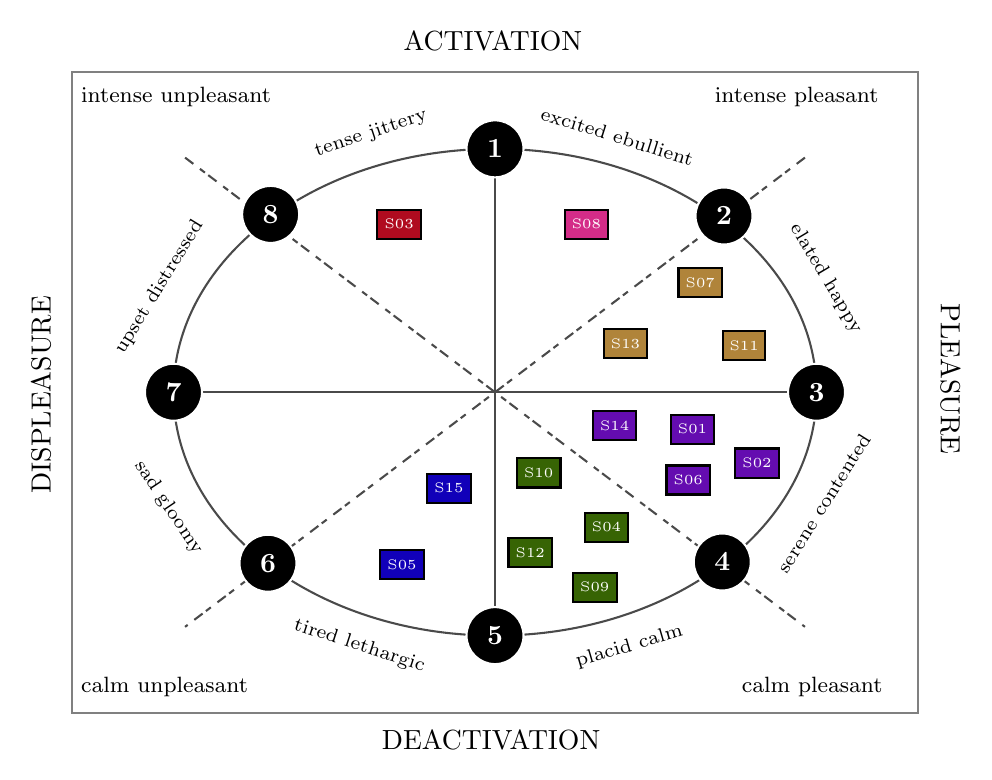
\begin{tikzpicture}[x=0.75pt,y=0.75pt,yscale=-1,xscale=1]
%uncomment if require: \path (0,389); %set diagram left start at 0, and has height of 389

%Flowchart: Or [id:dp3592995680476845] 
\draw  [color={rgb, 255:red, 74; green, 74; blue, 74 }  ,draw opacity=1 ] (182.64,181.1) .. controls (182.64,116.34) and (252,63.84) .. (337.55,63.84) .. controls (423.11,63.84) and (492.46,116.34) .. (492.46,181.1) .. controls (492.46,245.86) and (423.11,298.36) .. (337.55,298.36) .. controls (252,298.36) and (182.64,245.86) .. (182.64,181.1) -- cycle ; \draw  [color={rgb, 255:red, 74; green, 74; blue, 74 }  ,draw opacity=1 ] (182.64,181.1) -- (492.46,181.1) ; \draw  [color={rgb, 255:red, 74; green, 74; blue, 74 }  ,draw opacity=1 ] (337.55,63.84) -- (337.55,298.36) ;
%Straight Lines [id:da30798451784186187] 
\draw [color={rgb, 255:red, 74; green, 74; blue, 74 }  ,draw opacity=1 ] [dash pattern={on 3.75pt off 3pt on 2.25pt off 1.5pt}]  (188.22,68.06) -- (486.88,294.14) ;
%Straight Lines [id:da7804870395610348] 
\draw [color={rgb, 255:red, 74; green, 74; blue, 74 }  ,draw opacity=1 ] [dash pattern={on 3.75pt off 3pt on 2.25pt off 1.5pt}]  (486.88,68.06) -- (188.22,294.14) ;
%Shape: Rectangle [id:dp23344423808181314] 
\draw  [color={rgb, 255:red, 128; green, 128; blue, 128 }  ,draw opacity=1 ] (133.68,26.77) -- (541.42,26.77) -- (541.42,335.43) -- (133.68,335.43) -- cycle ;

% Text Node
\draw  [color={rgb, 255:red, 0; green, 0; blue, 0 }  ,draw opacity=1 ][fill={rgb, 255:red, 100; green, 12; blue, 176 }  ,fill opacity=1 ]  (453.29,208.22) -- (474.29,208.22) -- (474.29,222.22) -- (453.29,222.22) -- cycle  ;
\draw (463.79,215.22) node  [font=\tiny,color={rgb, 255:red, 255; green, 255; blue, 255 }  ,opacity=1 ] [align=left] {S02};
% Text Node
\draw  [color={rgb, 255:red, 0; green, 0; blue, 0 }  ,draw opacity=1 ][fill={rgb, 255:red, 176; green, 132; blue, 58 }  ,fill opacity=1 ]  (447.59,151.64) -- (467.59,151.64) -- (467.59,165.64) -- (447.59,165.64) -- cycle  ;
\draw (457.59,158.64) node  [font=\tiny,color={rgb, 255:red, 255; green, 255; blue, 255 }  ,opacity=1 ] [align=left] {S11};
% Text Node
\draw  [color={rgb, 255:red, 0; green, 0; blue, 0 }  ,draw opacity=1 ][fill={rgb, 255:red, 176; green, 11; blue, 31 }  ,fill opacity=1 ]  (280.87,93.11) -- (301.87,93.11) -- (301.87,107.11) -- (280.87,107.11) -- cycle  ;
\draw (291.37,100.11) node  [font=\tiny,color={rgb, 255:red, 255; green, 255; blue, 255 }  ,opacity=1 ] [align=left] {S03};
% Text Node
\draw  [color={rgb, 255:red, 0; green, 0; blue, 0 }  ,draw opacity=1 ][fill={rgb, 255:red, 176; green, 132; blue, 58 }  ,fill opacity=1 ]  (389.95,150.83) -- (410.95,150.83) -- (410.95,164.83) -- (389.95,164.83) -- cycle  ;
\draw (400.45,157.83) node  [font=\tiny,color={rgb, 255:red, 255; green, 255; blue, 255 }  ,opacity=1 ] [align=left] {S13};
% Text Node
\draw  [color={rgb, 255:red, 0; green, 0; blue, 0 }  ,draw opacity=1 ][fill={rgb, 255:red, 55; green, 100; blue, 4 }  ,fill opacity=1 ]  (375.12,267.99) -- (396.12,267.99) -- (396.12,281.99) -- (375.12,281.99) -- cycle  ;
\draw (385.62,274.99) node  [font=\tiny,color={rgb, 255:red, 255; green, 255; blue, 255 }  ,opacity=1 ] [align=left] {S09};
% Text Node
\draw  [color={rgb, 255:red, 0; green, 0; blue, 0 }  ,draw opacity=1 ][fill={rgb, 255:red, 100; green, 12; blue, 176 }  ,fill opacity=1 ]  (422.22,191.92) -- (443.22,191.92) -- (443.22,205.92) -- (422.22,205.92) -- cycle  ;
\draw (432.72,198.92) node  [font=\tiny,color={rgb, 255:red, 255; green, 255; blue, 255 }  ,opacity=1 ] [align=left] {S01};
% Text Node
\draw  [color={rgb, 255:red, 0; green, 0; blue, 0 }  ,draw opacity=1 ][fill={rgb, 255:red, 17; green, 0; blue, 185 }  ,fill opacity=1 ]  (282.25,257.14) -- (303.25,257.14) -- (303.25,271.14) -- (282.25,271.14) -- cycle  ;
\draw (292.75,264.14) node  [font=\tiny,color={rgb, 255:red, 255; green, 255; blue, 255 }  ,opacity=1 ] [align=left] {S05};
% Text Node
\draw  [color={rgb, 255:red, 0; green, 0; blue, 0 }  ,draw opacity=1 ][fill={rgb, 255:red, 55; green, 100; blue, 4 }  ,fill opacity=1 ]  (380.76,239.11) -- (401.76,239.11) -- (401.76,253.11) -- (380.76,253.11) -- cycle  ;
\draw (391.26,246.11) node  [font=\tiny,color={rgb, 255:red, 255; green, 255; blue, 255 }  ,opacity=1 ] [align=left] {S04};
% Text Node
\draw  [color={rgb, 255:red, 0; green, 0; blue, 0 }  ,draw opacity=1 ][fill={rgb, 255:red, 17; green, 0; blue, 185 }  ,fill opacity=1 ]  (304.83,220.33) -- (325.83,220.33) -- (325.83,234.33) -- (304.83,234.33) -- cycle  ;
\draw (315.33,227.33) node  [font=\tiny,color={rgb, 255:red, 255; green, 255; blue, 255 }  ,opacity=1 ] [align=left] {S15};
% Text Node
\draw  [color={rgb, 255:red, 0; green, 0; blue, 0 }  ,draw opacity=1 ][fill={rgb, 255:red, 100; green, 12; blue, 176 }  ,fill opacity=1 ]  (420.18,216.39) -- (441.18,216.39) -- (441.18,230.39) -- (420.18,230.39) -- cycle  ;
\draw (430.68,223.39) node  [font=\tiny,color={rgb, 255:red, 255; green, 255; blue, 255 }  ,opacity=1 ] [align=left] {S06};
% Text Node
\draw  [color={rgb, 255:red, 0; green, 0; blue, 0 }  ,draw opacity=1 ][fill={rgb, 255:red, 212; green, 44; blue, 136 }  ,fill opacity=1 ]  (371.1,93.11) -- (392.1,93.11) -- (392.1,107.11) -- (371.1,107.11) -- cycle  ;
\draw (381.6,100.11) node  [font=\tiny,color={rgb, 255:red, 255; green, 255; blue, 255 }  ,opacity=1 ] [align=left] {S08};
% Text Node
\draw  [color={rgb, 255:red, 0; green, 0; blue, 0 }  ,draw opacity=1 ][fill={rgb, 255:red, 55; green, 100; blue, 4 }  ,fill opacity=1 ]  (348.11,212.99) -- (369.11,212.99) -- (369.11,226.99) -- (348.11,226.99) -- cycle  ;
\draw (358.61,219.99) node  [font=\tiny,color={rgb, 255:red, 255; green, 255; blue, 255 }  ,opacity=1 ] [align=left] {S10};
% Text Node
\draw  [color={rgb, 255:red, 0; green, 0; blue, 0 }  ,draw opacity=1 ][fill={rgb, 255:red, 100; green, 12; blue, 176 }  ,fill opacity=1 ]  (384.68,190.21) -- (405.68,190.21) -- (405.68,204.21) -- (384.68,204.21) -- cycle  ;
\draw (395.18,197.21) node  [font=\tiny,color={rgb, 255:red, 255; green, 255; blue, 255 }  ,opacity=1 ] [align=left] {S14};
% Text Node
\draw  [color={rgb, 255:red, 0; green, 0; blue, 0 }  ,draw opacity=1 ][fill={rgb, 255:red, 55; green, 100; blue, 4 }  ,fill opacity=1 ]  (344.03,251.28) -- (365.03,251.28) -- (365.03,265.28) -- (344.03,265.28) -- cycle  ;
\draw (354.53,258.28) node  [font=\tiny,color={rgb, 255:red, 255; green, 255; blue, 255 }  ,opacity=1 ] [align=left] {S12};
% Text Node
\draw  [color={rgb, 255:red, 0; green, 0; blue, 0 }  ,draw opacity=1 ][fill={rgb, 255:red, 176; green, 132; blue, 58 }  ,fill opacity=1 ]  (425.94,121.16) -- (446.94,121.16) -- (446.94,135.16) -- (425.94,135.16) -- cycle  ;
\draw (436.44,128.16) node  [font=\tiny,color={rgb, 255:red, 255; green, 255; blue, 255 }  ,opacity=1 ] [align=left] {S07};
% Text Node
\draw  [color={rgb, 255:red, 255; green, 255; blue, 255 }  ,draw opacity=1 ][fill={rgb, 255:red, 0; green, 0; blue, 0 }  ,fill opacity=1 ]  (337.55, 63.84) circle [x radius= 13.73, y radius= 13.73]   ;
\draw (337.55,63.84) node  [font=\normalsize,color={rgb, 255:red, 255; green, 255; blue, 255 }  ,opacity=1 ] [align=left] {\textbf{1}};
% Text Node
\draw  [color={rgb, 255:red, 255; green, 255; blue, 255 }  ,draw opacity=1 ][fill={rgb, 255:red, 0; green, 0; blue, 0 }  ,fill opacity=1 ]  (447.88, 96.18) circle [x radius= 13.73, y radius= 13.73]   ;
\draw (447.88,96.18) node  [font=\normalsize,color={rgb, 255:red, 255; green, 255; blue, 255 }  ,opacity=1 ] [align=left] {\textbf{2}};
% Text Node
\draw  [color={rgb, 255:red, 255; green, 255; blue, 255 }  ,draw opacity=1 ][fill={rgb, 255:red, 0; green, 0; blue, 0 }  ,fill opacity=1 ]  (492.46, 181.1) circle [x radius= 13.73, y radius= 13.73]   ;
\draw (492.46,181.1) node  [font=\normalsize,color={rgb, 255:red, 255; green, 255; blue, 255 }  ,opacity=1 ] [align=left] {\textbf{3}};
% Text Node
\draw  [color={rgb, 255:red, 255; green, 255; blue, 255 }  ,draw opacity=1 ][fill={rgb, 255:red, 0; green, 0; blue, 0 }  ,fill opacity=1 ]  (447.05, 262.88) circle [x radius= 13.73, y radius= 13.73]   ;
\draw (447.05,262.88) node  [font=\normalsize,color={rgb, 255:red, 255; green, 255; blue, 255 }  ,opacity=1 ] [align=left] {\textbf{4}};
% Text Node
\draw  [color={rgb, 255:red, 255; green, 255; blue, 255 }  ,draw opacity=1 ][fill={rgb, 255:red, 0; green, 0; blue, 0 }  ,fill opacity=1 ]  (337.55, 298.36) circle [x radius= 13.73, y radius= 13.73]   ;
\draw (337.55,298.36) node  [font=\normalsize,color={rgb, 255:red, 255; green, 255; blue, 255 }  ,opacity=1 ] [align=left] {\textbf{5}};
% Text Node
\draw  [color={rgb, 255:red, 255; green, 255; blue, 255 }  ,draw opacity=1 ][fill={rgb, 255:red, 0; green, 0; blue, 0 }  ,fill opacity=1 ]  (228.16, 263.49) circle [x radius= 13.73, y radius= 13.73]   ;
\draw (228.16,263.49) node  [font=\normalsize,color={rgb, 255:red, 255; green, 255; blue, 255 }  ,opacity=1 ] [align=left] {\textbf{6}};
% Text Node
\draw  [color={rgb, 255:red, 255; green, 255; blue, 255 }  ,draw opacity=1 ][fill={rgb, 255:red, 0; green, 0; blue, 0 }  ,fill opacity=1 ]  (182.64, 181.1) circle [x radius= 13.73, y radius= 13.73]   ;
\draw (182.64,181.1) node  [font=\normalsize,color={rgb, 255:red, 255; green, 255; blue, 255 }  ,opacity=1 ] [align=left] {\textbf{7}};
% Text Node
\draw  [color={rgb, 255:red, 255; green, 255; blue, 255 }  ,draw opacity=1 ][fill={rgb, 255:red, 0; green, 0; blue, 0 }  ,fill opacity=1 ]  (229.45, 95.43) circle [x radius= 13.73, y radius= 13.73]   ;
\draw (229.45,95.43) node  [font=\normalsize,color={rgb, 255:red, 255; green, 255; blue, 255 }  ,opacity=1 ] [align=left] {\textbf{8}};
% Text Node
\draw (112.89,231.39) node [anchor=north west][inner sep=0.75pt]  [rotate=-270] [align=left] {DISPLEASURE};
% Text Node
\draw (292.08,5.96) node [anchor=north west][inner sep=0.75pt]   [align=left] {ACTIVATION};
% Text Node
\draw (281.58,342.71) node [anchor=north west][inner sep=0.75pt]   [align=left] {DEACTIVATION};
% Text Node
\draw (562.94,136.89) node [anchor=north west][inner sep=0.75pt]  [rotate=-90] [align=left] {PLEASURE};
% Text Node
\draw (150.9,160.23) node [anchor=north west][inner sep=0.75pt]  [font=\scriptsize,rotate=-301.49] [align=left] {upset distressed};
% Text Node
\draw (247.79,60.45) node [anchor=north west][inner sep=0.75pt]  [font=\scriptsize,rotate=-341.6] [align=left] {tense jittery};
% Text Node
\draw (359.94,41.46) node [anchor=north west][inner sep=0.75pt]  [font=\scriptsize,rotate=-17.34] [align=left] {excited ebullient};
% Text Node
\draw (485.75,96.5) node [anchor=north west][inner sep=0.75pt]  [font=\scriptsize,rotate=-59.2] [align=left] {elated happy};
% Text Node
\draw (470.66,265.95) node [anchor=north west][inner sep=0.75pt]  [font=\scriptsize,rotate=-301.93] [align=left] {serene contented};
% Text Node
\draw (373.68,306.2) node [anchor=north west][inner sep=0.75pt]  [font=\scriptsize,rotate=-343.65] [align=left] {placid calm};
% Text Node
\draw (241.21,287.33) node [anchor=north west][inner sep=0.75pt]  [font=\scriptsize,rotate=-18.04] [align=left] {tired lethargic};
% Text Node
\draw (169.56,210.51) node [anchor=north west][inner sep=0.75pt]  [font=\scriptsize,rotate=-56.13] [align=left] {sad gloomy};
% Text Node
\draw (455,317) node [anchor=north west][inner sep=0.75pt]  [font=\footnotesize] [align=left] {calm pleasant};
% Text Node
\draw (136.67,317) node [anchor=north west][inner sep=0.75pt]  [font=\footnotesize] [align=left] {calm unpleasant};
% Text Node
\draw (136.67,32.78) node [anchor=north west][inner sep=0.75pt]  [font=\footnotesize] [align=left] {intense unpleasant};
% Text Node
\draw (442,32.78) node [anchor=north west][inner sep=0.75pt]  [font=\footnotesize] [align=left] {intense pleasant};


\end{tikzpicture}

    \fonte{Author.}
\end{figure}

% O formulário \ac{sus} aplicado baseou-se no seu formato clássico, com dez (10) afirmações com uma escala Likert associada.
% Esta escala vai de um (1) até cinco (5).
% As dez (10) afirmações que os sujeitos avaliaram eram as seguintes:
The \ac{sus} form was applied based on its classic format, with ten (10) statements with an associated Likert~\cite{Likert} scale.
This scale goes from one (1) to five (5).
The ten (10) statements that the subjects rated were as follows:

% !!!!!!!!!!!!!!!!!!!!!!!!!!!!!!!!!!!!!!!!!!!!!!!!!!!!!!!!!!!!!!!!!
% !! Fazer tabela para condensar invformações, deixar \scriptsize!!
% !!!!!!!!!!!!!!!!!!!!!!!!!!!!!!!!!!!!!!!!!!!!!!!!!!!!!!!!!!!!!!!!!
% \begin{enumerate}
%     \item {\scriptsize \textit{I think that I would like to use this solution frequently.}}
%     \item {\scriptsize \textit{I found the solution unnecessarily complex.}}
%     \item {\scriptsize \textit{I thought the solution was easy to use.}}
%     \item {\scriptsize \textit{I think that I would need the support of a technical person to be able to use this solution.}}
%     \item {\scriptsize \textit{I found the various functions in this solution were well integrated.}}
%     \item {\scriptsize \textit{I thought there was too much inconsistency in this solution.}}
%     \item {\scriptsize \textit{I would imagine that most people would learn to use this solution very quickly.}}
%     \item {\scriptsize \textit{I found the solution very cumbersome to use.}}
%     \item {\scriptsize \textit{I felt very confident using the solution.}}
%     \item {\scriptsize \textit{I needed to learn a lot of things before I could get going with this solution.}}
% \end{enumerate}

\rowcolors{1}{gray!15}{white}
\begin{table}[!htb]
    \caption{SUS statements.}
    \label{tab:SUSstatements}
    \centering
    \scriptsize
    \begin{tabular}{ll}
    \rowcolor[HTML]{C0C0C0}
    \bottomrule
    \textbf{\#} & \textbf{SUS STATEMENTS} \\ \hline
    01 & I think that I would like to use this solution frequently. \\
    02 & I found the solution unnecessarily complex. \\
    03 & I thought the solution was easy to use. \\
    04 & I think that I would need the support of a technical person to be able to use this solution. \\
    05 & I found that the various functions in this solution were well integrated. \\
    06 & I thought there was too much inconsistency in this solution. \\
    07 & I would imagine that most people would learn to use this solution very quickly. \\
    08 & I found the solution very cumbersome to use. \\
    09 & I felt very confident using the solution. \\
    10 & I needed to learn a lot of things before I could get going with this solution. \\ \toprule
    \end{tabular}
    \fonte{\cite{sus:1995}.}
\end{table}

% Este método pode ser usado para avaliar produtos, serviços, hardware, software, websites, aplicações e qualquer outro tipo de interface. 
% Os critérios este método ajuda a availar abrangem:
We can use this method to evaluate products, services, hardware, software, websites, applications, and any other type of interface.
%This method can be used to evaluate products, services, hardware, software, websites, applications and any other type of interface.
The criteria this method helps to assess cover are: (i) Effectiveness (can users complete their objectives?); (ii) Efficiency (how much effort and resources are needed for this?); and (iii) Satisfaction (was the experience satisfactory?).

% \begin{enumerate} [label=\roman*.]
    % \item Efetividade (os usuários conseguem completar seus objetivos?);
    % \item Effectiveness (can users complete their objectives?);
    % \item Eficiência (quanto esforço e recursos são necessários para isso?);
    % \item Efficiency (how much effort and resources are needed for this?);
    % \item Satisfação (a experiência foi satisfatória?).
    % \item Satisfaction (was the experience satisfactory?).
% \end{enumerate}

% O cálculo do score para cada afirmação se dá através de uma equação simples.
% As afirmações que são ímpares (1, 3, 5, 7, 9) é necessário se subtrair 1 do valor da escala Likert escolhida pelo participante. 
% Por exemplo, a afirmação 5 foi avaliada como 4, logo 4 \textminus~1 = 3.
We calculated the score for each statement using a simple equation.
%The score for each statement is calculated using a simple equation.
The odd statements (1, 3, 5, 7, 9) need to be subtracted 1 (one) from the Likert~\cite{Likert} scale value chosen by the participant.
%The statements that are odd (1, 3, 5, 7, 9) need to be subtracted 1 from the Likert scale value chosen by the participant.
For example, statement 5 evaluated as 4, so 4\textminus1=3.

% Para as afirmações pares (2, 4, 6, 8, 10) é necessário que o valor escolhido na escala Likert seja subtraído de 5.
% Por exemplo, digamos que na afirmação 4 o valor escolhido é 3. 
% Então, se tem 5 \textminus~3 = 2. 
% Com os valores individuais de cada afirmação calculados, deve-se somar tudo e multiplicar por 2,5.
% Os valores obtidos devem então ser somados e divididos por 10, chegando-se assim no valor final geral correspondente.
For even statements (2, 4, 6, 8, 10), the value must choose on the Likert scale subtracted from 5.
%For even statements (2, 4, 6, 8, 10) it is necessary that the value chosen on the Likert scale be subtracted from 5.
For example, let's say that in statement 4, the value chosen is 3.
So if you have 5\textminus3=2.
With the individual values of each statement calculated, add them all together and multiply by 2.5.
The values obtained must then be added and divided by 10, thus arriving at the corresponding final general value.

% A Tabela \ref{tab:ResultsSUS} apresenta os valores finais obtidos.
% Pode-se obeservar que houve um máximo de 100 para ambas as abordagens, e um mínimo de 37,50 para a abordagem gráfica, enquanto a abordagem textual teve 50,00.
% Os valores médios totais ficaram muito parecidos, sendo 76,83 e 78,50 para as abordagens gráfica e textual, respectivamente. 
% A Figura \ref{fig:BoxPlotSUS_tools} apresenta o gráfico de dispersão dos resultados finais.
Table \ref{tab:ResultsSUS} presents the final values obtained.
It can see that both approaches reached a maximum of 100 and a minimum of 37.50 for the graphical, while the textual one had 50.00.
%It can be seen that there was a maximum of 100 for both approaches, and a minimum of 37.50 for the graphical approach, while the textual approach had 50.00.
The total average values were very similar, whose values are 76.83 and 78.50, respectively, for the graphical and textual approaches.
%The total average values were very similar, being 76.83 and 78.50 for the graphic and textual approaches, respectively.
Figure \ref{fig:BoxPlotSUS_tools} shows the box-plot of the final results.

\rowcolors{1}{gray!15}{white}
\begin{table}[!htb]
    \caption{Measures of the SUS values in EX3.}
    \label{tab:ResultsSUS}
    \centering
    \scriptsize
    % \tiny
    \begin{tabular}{l|ccccc|ccccc}%{l|ccccc|ccccc}
    \bottomrule
    \rowcolor[HTML]{C0C0C0}
    \multicolumn{1}{l}{} &
    \multicolumn{1}{c|}{\textbf{Graphical Treatment}} &
    \multicolumn{1}{c}{\textbf{Textual Treatment}}
    \\ 
    \hline
    \rowcolor[HTML]{C0C0C0}
    \textbf{Measure} & \textbf{SUS Final Score} & \textbf{SUS Final Score}
    \\
    \hline
Maximum	&	100.00	&	100.00		\\
3\textdegree Quartile	&	85.00	&	92.50	\\
Average	&	76.83	&	78.50	\\
Median	&	80.00	&	75.00	\\
1\textdegree Quartile	&	73.75	&	67.50	\\
Minimum	&	37.50	&	50.00	\\
Variance	&	248.63	&	241.79	\\
SD	&	15.77	&	15.55	\\
    \toprule
\end{tabular}
\begin{tablenotes}
    \scriptsize
    \centering
    \item \textit{Legend: SD = Standard Deviation.}
\end{tablenotes}
\fonte{Author.}
\end{table}

% Para comparação final, os resultados médios apresentados classificam as duas ferramentas dentro da faixa que diz respeito ao conceito de bom quanto a sua usabilidade.
% A Tabela \ref{tab:GradesSUS} apresenta a tabela com adjetivos que podem ser atribuídos aos artefatos avaliados utilizando o método \ac{sus}.
For a final comparison, the average results presented classify the two tools within the range that concerns the concept of good in terms of their usability.
Table \ref{tab:GradesSUS} presents the table with adjectives that can be assigned to the evaluated artifacts using the \ac{sus} method.

\rowcolors{1}{gray!15}{white}
\begin{table}[!htb]
\centering
\scriptsize
\caption{SUS classification.}
\label{tab:GradesSUS}
\begin{tabular}{ccc}
\bottomrule
\rowcolor[HTML]{C0C0C0}
\textbf{SUS Score} & \textbf{Grade} & \textbf{Adjective Rating} \\ \hline
\textgreater~80.3 & \cellcolor[HTML]{34A853}A & Excellent \\
68 - 80.3 & \cellcolor[HTML]{93C47D}B & Good \\
68 & \cellcolor[HTML]{FFFF00}C & Okay \\
51 - 68 & \cellcolor[HTML]{FBBC04}D & Poor \\
\textless~51 & \cellcolor[HTML]{EA4335}E & Awful \\
\toprule
\end{tabular}
\fonte{Adapted from~\cite{sus:1995}.}
\end{table}

\begin{figure}[!htb]
    \centering
    \caption{Box-plot - SUS score per treatments in EX3.}
    \label{fig:BoxPlotSUS_tools}
    \begin{filecontents*}{data5.csv}
37.5,50,72.5,72.5,75,75,75,80,80,82.5,85,85,87.5,95,100
50,60,67.5,67.5,67.5,70,70,75,80,90,92.5,92.5,97.5,97.5,100
\end{filecontents*}

\makeatletter
\pgfplotsset{
    boxplot/hide outliers/.code={
        \def\pgfplotsplothandlerboxplot@outlier{}%
    }
}
\makeatother

\begin{tikzpicture}
    \pgfplotstableread[col sep=comma]{data5.csv}\csvdata
    % Boxplot groups columns, but we want rows
    \pgfplotstabletranspose\datatransposed{\csvdata} 
    \begin{axis}[
         boxplot/draw direction=y,
        xtick={1, 2},
        ylabel={\scriptsize Percentage (\%)},
        xticklabels={{\scriptsize Graphical Treatment}, {\scriptsize Textual Treatment}},
        height=7cm,
        width=10cm,
        % boxplot/draw direction = y,
        % axis x line* = bottom,
        % axis y line = left,
        % enlarge y limits,
        ymajorgrids,
        % xtick = {1, 2},
        % xticklabel style = {align=center, font=\small},
        % xticklabels = {Graphical Treatment, Textual Treatment},
        % ylabel = {Percentage (\%)},
        ytick = {40, 50, 60, 70, 80, 90},
        yticklabel style = {font=\scriptsize}
    ]
        \foreach \n in {1,...,2} {
            \addplot+[boxplot, fill, fill opacity=0.4, draw=black] table[y index=\n] {\datatransposed};
        }
    \end{axis}
\end{tikzpicture}

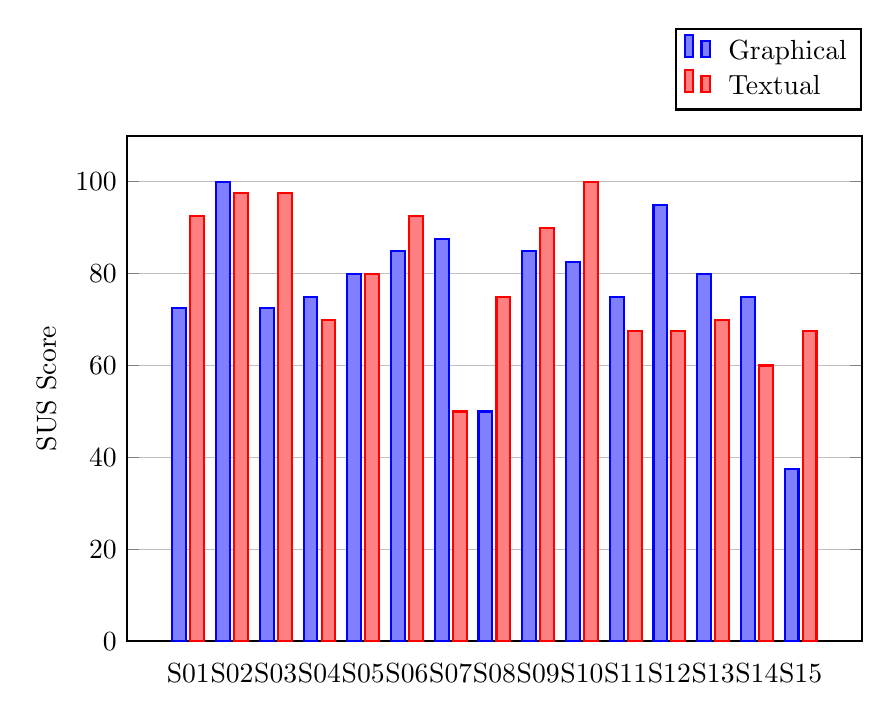
\begin{tikzpicture}
    \begin{axis}[
        width  = 0.90\textwidth,
        height = 8cm,
        major x tick style = transparent,
        ybar=2*\pgflinewidth,
        bar width=5pt,
        ymajorgrids = true,
        ylabel = {SUS Score},
        symbolic x coords={
        S01, S02, S03, S04, S05, S06, S07, S08, S09, S10, S11, S12, S13, S14, S15
        },
        xtick = data,
        scaled y ticks = false,
        % enlarge x limits=0.20,
        ymin=0,
        legend cell align=left,
        legend style={
                at={(1,1.05)},
                anchor=south east,
                column sep=1ex
        }
    ]
        \addplot[style={blue,fill=blue!50}]
            coordinates {
            (S01,72.5) (S02,100) (S03,72.5) (S04,75) (S05,80) (S06,85) (S07,87.5) (S08,50) (S09,85) (S10,82.5) (S11,75) (S12,95) (S13,80) (S14,75) (S15,37.5)
            };

        \addplot[style={red,fill=red!50}]
            coordinates {
            (S01,92.5) (S02,97.5) (S03,97.5) (S04,70) (S05,80) (S06,92.5) (S07,50) (S08,75) (S09,90) (S10,100) (S11,67.5) (S12,67.5) (S13,70) (S14,60) (S15,67.5)
            };
            
        \legend{Graphical,Textual}
    \end{axis}
\end{tikzpicture}

    \fonte{Author.}
\end{figure}

% Um gráfico de barras agrupadas é apresentado na Figura \ref{fig:GroupedBarSUS_tools} apresenta os valores obtidos por cada um dos quinze (15) indivíduos para cada uma das abordagens.
% É díficil avaliar uma relação de causa e efeito que seja equivalente entre os valores obtidos no cálculo \ac{sus}, mas é possível fazer algumas inferências.
Figure \ref{fig:GroupedBarSUS_tools} shows a chart of grouped bars and presents the values obtained by each one of fifteen (15) individuals for both approaches.
%A chart of grouped bars is shown in Figure \ref{fig:GroupedBarSUS_tools}, and presents the values obtained by each of the fifteen (15) individuals for each of the approaches.
It is ambitious to evaluate a cause and effect relationship equivalent to the values obtained in the \ac{sus} calculation, but it is possible to make some inferences.
%It is difficult to evaluate a cause and effect relationship that is equivalent between the values obtained in the \ac{sus} calculation, but it is possible to make some inferences.

% Por exemplo, o Sujeito 03 demonstrou que se sentia com um sentimento de irritabilidade enquanto utilizava a ferramenta brModelo, enquanto estava em um aspecto de emoção ligada a felicidade no uso da ferramenta ERtext.
% Isso se traduziu na avaliação do \ac{sus}, uma vez que o sujeito avaliou de melhor forma a abordagem textual frente a abordagem gráfica.
For example, subject S03 demonstrated that he felt a feeling of irritability while using the brModelo tool, while he was in an aspect of emotion linked to happiness in the use of the ERtext tool. 
We translated this evidence in the \ac{sus} evaluation since the subject better evaluated the textual approach when compared to the graphical one.
%This resulted in the evaluation of \ac{sus}, since the subject better evaluated the textual approach compared to the graphic approach.

% Este padrão acontece mais vezes, mas em outras ocorrências não há essa equivalência.
% É o caso do Sujeito 07, que declarou estar sentindo emoções ligadas as irritabilidade durante o uso da abordagem textual, enquanto se sentia no espectro de emoções felizes na abordagem gráfica.
% De forma contraditória, na valor \ac{sus} calculado para este elemento há uma avaliação muito melhor para a abordagem gráfica utilizando a ferramenta brModelo, enquanto a abordagem textual utilizando a solução proposta ERtext recebeu um dos menores valores do \ac{sus}. 
% Contudo, de modo geral, os valores obtidos da maioria dos outros participantes correspondem a sensação relatada para o estado de espírito que eles sentiam no momento.
This pattern happens more often, but there is no such equivalence in other instances.
%This pattern happens at other times, but in other instances there is no such equivalence.
For instance, the case of subject S07, who declared that he was feeling emotions linked to irritability during the textual approach utilization while feeling on the spectrum of happy emotion in the graphical one.
%This is the case of Subject 07, who declared that he was feeling emotions linked to irritability during the use of the textual approach, while feeling on the spectrum of happy emotions in the graphic approach.
In a contradictory way, in the value \ac{sus} calculated for this subject, there is a much better evaluation for the graphical approach using the brModelo tool, while the textual one using the proposed solution ERtext received one of the lowest values of \ac{sus}.
However, in general, the values obtained from most other participants correspond to the sensation reported for the state of mind they were feeling at the time.

\begin{figure}[!htb]
    \centering
    \caption{Grouped Bar Chart - SUS score per subjects and treatments.}
    \label{fig:GroupedBarSUS_tools}
    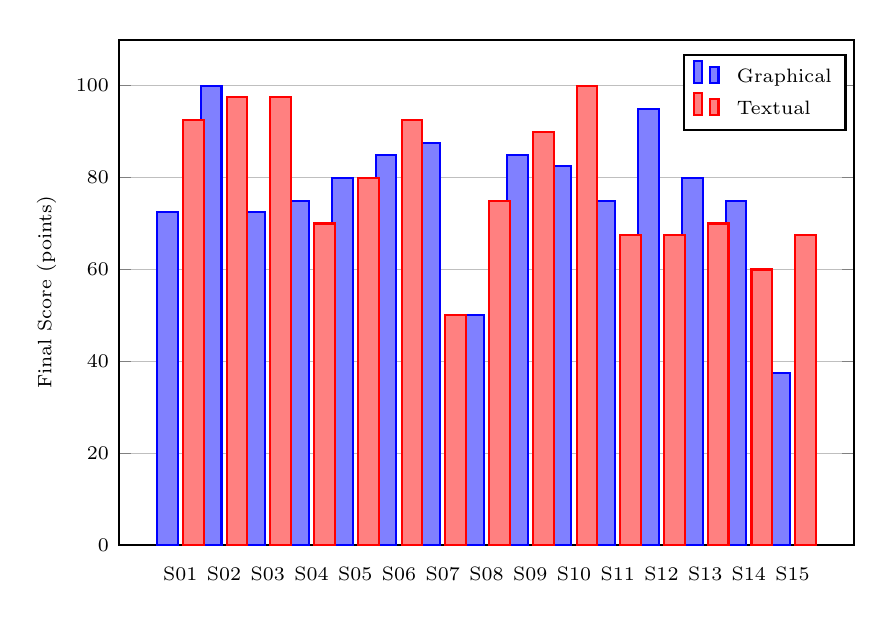
\begin{tikzpicture}
    \begin{axis}[
        width  = 0.90\textwidth,
        height = 8cm,
        major x tick style = transparent,
        ybar=2.5*\pgflinewidth,
        bar width=7.5pt,
        ymajorgrids = true,
        ylabel = {Final Score (points)},
        symbolic x coords={
        S01, S02, S03, S04, S05, S06, S07, S08, S09, S10, S11, S12, S13, S14, S15
        },
        xtick = data,
        scaled y ticks = false,
        % enlarge x limits=0.20,
        ymin=0,
        label style={font=\scriptsize},
        tick label style={font=\scriptsize},
        legend cell align=left,
        legend style={
                at={(0.99,0.82)},
                anchor=south east,
                column sep=1ex,
                font = \scriptsize
        }
    ]
        \addplot[style={blue,fill=blue!50}]
            coordinates {
            (S01,72.5) (S02,100) (S03,72.5) (S04,75) (S05,80) (S06,85) (S07,87.5) (S08,50) (S09,85) (S10,82.5) (S11,75) (S12,95) (S13,80) (S14,75) (S15,37.5)
            };

        \addplot[style={red,fill=red!50}]
            coordinates {
            (S01,92.5) (S02,97.5) (S03,97.5) (S04,70) (S05,80) (S06,92.5) (S07,50) (S08,75) (S09,90) (S10,100) (S11,67.5) (S12,67.5) (S13,70) (S14,60) (S15,67.5)
            };
            
        \legend{Graphical,Textual}
    \end{axis}
\end{tikzpicture}
    \fonte{Author.}
\end{figure}

% Para a avaliação das questões abertas houve um processo de codificação das respostas dadas nos intrumentos de avaliação.
% Neste momento foi utilizada a ferramenta de análise qualitativa QAnubis\footnote{QAnubis tool: \url{http://168.138.132.249/}}.
% Esta ferramenta Web tem por objetivo apoiar o processo de análise qualitativa por meio da criação de códigos e anotações sobre arquivos PDF, gerando relatórios capazes de sumarizar os conceitos capturados.
For the evaluation of open-ended questions, there was a process of coding the answers given in the evaluation instruments.
At this moment, we used the qualitative analysis tool QAnubis\footnote{QAnubis tool: We received early access for testing only, public access link is unavailable currently.}.
This web tool aims to support the qualitative analysis process by creating codings and annotations directly on PDF files, generating reports capable of summarizing the captured concepts.

% Foram cerca de setenta (70) respostas curtas em formato aberto, uma vez que cada um dos quinze (15) participantes podiam dar suas impressões sobre os artefatos gerados nos três (3) níveis de modelagem, para cada uma das duas (2) abordagens.
There were about seventy (70) short answers in an open-ended format since each of the fifteen (15) participants could give their impressions about the artifacts generated in the three (3) modeling levels for each of the two (2) approaches.

% Os códigos definidos foram Positive Feedback, Negative Feedback, Neutral Feedback, Improvements e Feature Idea.
% Como mencionado anteriormente, estas perguntas abertas pediam critícas, elogios, dúvidas ou sugestões de melhoria quando os participantes achassem interessante realizar o relato.
The codes defined were Positive Feedback, Negative Feedback, Neutral Feedback, Improvements, and Feature Idea.
As aforementioned, when participants found it interesting to report for criticism, compliments, questions, or suggestions for improvement, they answered the open-ended questions.
%As mentioned earlier, these open-ended questions asked for criticism, compliments, questions, or suggestions for improvement when participants found it interesting to report.

% Os elogios e relatos de experiência satisfatória ficaram categorizados como Positive Feedback.
% Algumas críticas, quando não mencionassem melhorias ou apontassem problemas de funcionamento de alguma característica das ferramentas, eram categorizadas como Negative feedback.
% As respostas que indicassem que não havia sugestões, críticas ou elogios, apenas relatando opiniões vagas ou ambíguas, eram então classificadas como Neutral Feedback.
We categorized compliments and reports of satisfactory experience as Positive Feedback.
% Compliments and reports of satisfactory experience were categorized as Positive Feedback.
Further, we classified as Negative Feedback some criticisms when they did not mention improvements or pointed out malfunctions of some features of the tools.
% Some criticisms, when they did not mention improvements or pointed out malfunctions of some feature of the tools, were categorized as Negative feedback.
Furthermore, we grouped Neutral Feedback responses that indicated that there were no suggestions, criticisms, or compliments, only reporting vague or ambiguous opinions.
% Responses that indicated that there were no suggestions, criticisms or compliments, only reporting vague or ambiguous opinions, were then classified as Neutral Feedback.

% As respostas que indicassem problemas quanto a funcionalidades que não operavam corretamente, conforme o esperado pelo usuário, foram classificadas como Improvements.
% Finalmente, os relatos de possíveis funcionalidades não existentes e que poderiam ser implementadas foram categorizadas como Feature Idea.
Moreover, we classified as Improvements responses that indicated problems with functionality that did not operate correctly, as expected by the user.
%Responses that indicated problems with functionality that did not operate correctly, as expected by the user, were classified as Improvements.
Finally, we categorized as Feature Ideas reports of possible non-existent features that could implement.
%Finally, reports of possible non-existent features that could be implemented were categorized as Feature Idea.

% A Tabela \ref{tab:QAnubis} apresenta a quantidade de ocorrências de cada código nas respostas analisadas, conforme a abordagem a qual pertenciam.
Table \ref{tab:QAnubis} shows the number of occurrences of each coding in the analyzed responses, according to the approach to which they belonged.

\rowcolors{1}{gray!15}{white}
\begin{table}[!htb]
 \caption{Occurrences of codings per treatments in EX3.}
    \label{tab:QAnubis}
\scriptsize
\centering
\begin{tabular}{rccccc}
\bottomrule
\rowcolor[HTML]{C0C0C0}
\textbf{Approach} & \textbf{Positive F.} & \textbf{Neutral F.} & \textbf{Negative F.} & \textbf{Improvements} & \textbf{Feature Idea} \\ \hline
\textbf{Graphical} & 14 & 4 & 17 & 7 & 2 \\
\textbf{Textual} & 16 & 2 & 5 & 2 & 4 \\ \toprule
\end{tabular}
\begin{tablenotes}
    \scriptsize
    \centering
    \item \textit{Legend: F = Feedback.}
\end{tablenotes}
\fonte{Author.}
\end{table}

% Foi realizado o mapeamento dos respondentes conforme feito para as respostas referentes aos Emocards e formulário \ac{sus}.
% Dessa forma é possível citar, por exemplo, que o Sujeito 06 considerou a abordagem textual para modelagem conceitual eficiente e mais rápida que a abordagem gráfica.
% Este sujeito ainda cita ter achado um pouco confuso entender o modelo lógico textual gerado em um primeiro momento, mas ainda assim ter gostado do resultado final.
We mapped respondents as was done for the responses referring to Emocards and the SUS form.
%Respondents were mapped as was done for the responses referring to Emocards and the \ac{sus} form.
Therefore, for example, it is possible to mention that subject S06 considered the textual approach to conceptual modeling efficient and faster than the graphical one.
%Thus, it is possible to mention, for example, that Subject 06 considered the textual approach to conceptual modeling efficient and faster than the graphical approach.
This subject still mentions having found it a bit confusing to understand the logical textual model generated at first, but yet have liked the final result.
%This subject still mentions having found it a bit confusing to understand the logical textual model generated at first, but still having liked the final result.

% Outro exemplo é o Sujeito 12 que fornece a recomendação de que seria interessante uma funcionalidade que pudesse dar liberdade de escolher as cores do diagrama conceitual e modelo lógico textual na abordagem usada na ferramenta ERtext, algo que ele menciona estar presente na  brModelo.
Another example is subject S12, who recommends that it would be interesting to have a functionality that could offer customization of the colors of the conceptual diagram and textual logical model in the approach used in the ERtext tool, something he mentions being present in brModelo.

% O Sujeito 03 relata que a padronização utilizando elementos da \ac{uml} para o diagrama conceitual produzido pela ERtext era algo inesperado para ele, bem como a impossibilidade de reorganiza-lo.
% De outra forma, citou que o diagrama da brModelo, apesar de mais familiar com o aprendizado dele, apresentava alguns problemas para a organização automática dos elementos, o fazendo gastar mais tempo do que o esperado.
On the one hand, subject S03 reports that the standardization using elements from UML for the conceptual diagram produced by ERtext was anything unexpected for him as even the impossibility of reorganizing it.
%Subject S03 reports that the standardization using elements from \ac{uml} for the conceptual diagram produced by ERtext was something unexpected for him, as well as the impossibility of reorganizing it.
On the other hand, he mentioned that despite being more familiar with learning the brModelo diagram, he presented some problems with the automatic organization of the elements, making him spend more time than expected.
%On the other hand, he mentioned that the brModelo diagram, despite being more familiar with his learning, presented some problems for the automatic organization of the elements, making him spend more time than expected.

% As principais críticas, gerando classificações em Negative Feedacks, se deram em relação aos modelos físicos.
% O número maior foram a respeito do código \ac{sql} gerado pela ferramenta brModelo, que segundo muitos dos respondentes, precisou de pequenos ajustes para que fossem executados no \ac{dbms} exigido.
% Acreditamos que isso se deu em razão das instruções não serem focadas em uma plataforma \ac{dbms} específica, uma vez que no geral tem um teor mais genérico.
The main criticisms generating classifications in Negative Feedback were concerning the physical models.
%The main criticisms, generating classifications in Negative Feedacks, were in relation to the physical models.
We related the highest number to the \ac{sql} code generated by the brModelo tool. Many of the respondents needed minor adjustments to execute the required DBMS.
%The largest number was related to the \ac{sql} code generated by the brModelo tool, which, according to many of the respondents, needed small adjustments to be executed in the required \ac{dbms}.
We aim at obtaining enough shreds of evidence because the instructions are not focused on a specific \ac{dbms} platform since, in general, it has a more generic template.
%We believe that this is because the instructions are not focused on a specific \ac{dbms} platform, since in general it has a more generic template.

% Os Sujeitos 04, 07 e 14 ainda relataram haver problemas na geração das chaves estrangeiras, que precisaram ser analisadas e então modificadas para execução correta.
% Os mesmos problemas, entretanto, não foram relatados na abordagem textual utilizando a ERtext.
% Todos os dados brutos analisados no \ac{ex3} estão também disponíveis em um repositório\footnote{: link do repositório ex3 no Zenodo.} público na plataforma Zenodo.
Subjects S04, S07, and S14 still reported problems in the foreign keys generation, which had to be analyzed and then modified for correct execution.
However, we have not reported the same problems in the textual approach using ERtext.
%The same problems, however, were not reported in the textual approach using ERtext.
All raw data analyzed in \ac{ex3} is also available in a public repository\footnote{: link to ex3 repository on Zenodo.} on the Zenodo platform.

%------------------------------------------------------------------------------
\section{Chapter Lessons}
\label{sec_experiments:lessons}
%------------------------------------------------------------------------------

% Este capítulo apresentou uma replicação preliminar de um experimento controlado, chamado \ac{ex1}, com uma amostra de 33 sujeitos avaliando a proposta ERtext, uma proposta de ferramenta textual utilizando uma \ac{dsl} para modelagem conceitual do \acp{db}.
% Comparamos a ERtext com a brModelo, uma ferramenta de abordagem gráfica bastante conhecida nas aulas de Computação.
This chapter presented a preliminary replication of a controlled experiment, called \ac{ex1}, with a sample of 33 subjects evaluating the ERtext proposal, a proposed textual tool using \ac{dsl} for conceptual modeling of \acp{db} .
We compared ERtext with brModelo, a graphical approach tool well known in Computing classes.

% Em seguida, foram realizados mais outros dois experimentos.
% O \ac{ex2} foi uma nova replicação com algumas modificações no protocolo, especificamente a adição de instrumentos novos, e tendo desta vez vinte e cinco (25) participantes.
% O objetivo foi realizar uma nova análise do esforço e eficácia das abordagens com cada ferramenta. 
% Ainda buscou-se fazer uma avaliação mais profunda da qualidade no uso utilizando conceitos como o de circumplexo de Russel combinado com o método Emocards.
Then, two more experiments were carried out.
\ac{ex2} was a new replication with some modifications in the protocol, specifically the addition of new instruments, and this time having twenty-five (25) participants.
The objective was to carry out a new analysis of the effort and effectiveness of the approaches with each tool.
We also sought to make a deeper assessment of the quality of use by applying concepts of Russell's circumplex combined with the Emocards method.

% Finalmente, o \ac{ex3} foi outra nova execução do protocolo, agora com a adição do formulário \ac{sus} e de uma análise qualitativa por codificação.
% Este último experimento contou com quinze (15) participantes e objetivou avaliar os diversos artefatos (modelos conceituais, diagramas, modelos lógicos e instruções \ac{sql}) que podiam ser gerados por ambas as ferramentas.
Finally, \ac{ex3} was another new implementation of the protocol, now with the addition of the \ac{sus} form and a qualitative coding analysis.
This last experiment had fifteen (15) participants and aimed to evaluate the various artifacts (conceptual models, diagrams, logical models and \ac{sql} instructions) that could be generated by both tools.

% Desta forma chegou-se a um conjunto de três (3) avaliações empíricas com um total combinado de setenta e três (73) participantes. 
% Com os resultados obtidos, foi possível responder aos quatro QRs do experimento, bem como às duas hipóteses associadas.
% Nesse sentido, podemos dizer que investigamos três aspectos principais do nosso \ac{dsl}: esforço, eficácia e qualidade no uso.
In this way, a set of three (3) empirical evaluations was reached with a combined total of seventy-three (73) participants.
With the results obtained, it was possible to answer the four RQs of the experiment, as well as the two associated hypotheses.
In this sense, we can say that we investigated three main aspects of our \ac{dsl}: effort, effectiveness and quality in use.

% A partir da análise de todos os conjuntos de dados obtidos, é possível destacar os seguintes aspectos:
From the analysis of all datasets obtained, it is possible to highlight the following aspects:

% \item \textbf{Esforço:} A diferença média calculada nos experimentos constata que não há diferenças entre as abordagens, \textit{ie}, uma abordagem não é mais rápida que a outra.
\item \textbf{Effort:} The average difference calculated in the experiments concludes that there are no differences between the approaches, \textit{i.e.}, one approach is not faster than the other.

% \item \textbf{Eficácia:} Através do teste estatístico rejeitamos a hipótese nula de que as abordagens são igualmente eficazes no \ac{ex1}.
% Ao comparar os gráficos box-plot produzidos, é possível observar uma pequena vantagem para a abordagem textual de cerca de 5\% em média.
% Contudo, no \ac{ex2} observou-se que não houve diferenças estatisticamente significativas quanto aos artefatos modelados.
% Na realidade, o qualidade média teve uma diferença de cerca de pouco mais de 1\% no \ac{ex2}.
% Isso demonstra que de certa forma é possível se sustentar que ambas as abordagens são similares quanto a qualidade dos modelos produzidos, haja visto a baixa diferença percentual apreciada.
% Também não descartamos possíveis influências causadas pelo fato de os experimentos terem sido conduzidos remotamente por conta do contexto de pandemia.
\item \textbf{Efficacy:} Through the statistical test we reject the null hypothesis that the approaches are equally effective in \ac{ex1}.
When comparing the box-plot plots produced, it is possible to observe a small advantage for the textual approach of about 5\% on average.
However, in \ac{ex2} it was observed that there were no statistically significant differences regarding the modeled artifacts.
In fact, the average quality had a difference of about a little over 1\% on \ac{ex2}.
This demonstrates that in a way it is possible to sustain that both approaches are similar in terms of the quality of the models produced, given the low percentage difference appreciated.
We also don’t discard possible influences caused by the fact that the experiments were conducted remotely due to the pandemic context.

% \item \textbf{Comparação qualitativa entre tratamentos:} Observou-se certo equilíbrio entre os tratamentos, mas com avaliação positiva para ERtext quanto aos atributos ``Produtividade'' e ``Operabilidade'' no \ac{ex1}.
% A principal vantagem observada quanto a brModelo se deu no \ac{ex2} em relação ao atributo de ``aprendizibilidade''.
\item \textbf{Qualitative comparison between treatments:} There was a certain balance between treatments, but with a positive evaluation for ERtext regarding the attributes ``Productivity'' and ``Operability'' in \ac{ex1}.
The main advantage observed for brModelo occurred in \ac{ex2} in relation to the ``Learnability'' attribute.

% \item Também coletamos \textbf{feedback qualitativo}, inclusive na forma de \textbf{respostas abertas} de indivíduos que participaram dos experimentos:
% Como resultado, existem algumas melhorias em relação ao design da \ac{dsl} que precisam ser revisadas, em particular nos relacionamentos ternários (\ac{ex1} e \ac{ex2}) e autorrelações (\ac{ex1}).
% Quanto a codificação de respostas abertas recebidas no \ac{ex3}, conseguimos mapear algumas críticas e sugestões interessantes para o planejamento de uma evolução da ERtext, sobretudo quanto a criação dinâmica e personalização de diagramas equivalentes as descrições textuais.
\item We also collected \textbf{qualitative feedback}, including in the form of \textbf{open-ended responses} from subjects who participated in the experiments:
As a result, there are some improvements regarding the design of \ac{dsl} that need to be revised, in particular in the ternary relationships (\ac{ex1} and \ac{ex2}) and self-relationships (\ac{ex1}).
Concerning the coding of the responses of open-ended questions received in \ac{ex3}, we were able to map some interesting criticisms and suggestions for planning an evolution of ERtext, especially regarding the dynamic creation and customization of diagrams equivalent to textual descriptions.

% Uma vez que está prevista a continuidade do desenvolvimento do \ac{dsl}, a execução de uma possível refatoração, e também a implementação de novos construtores de ER, é um passo natural para a evolução do solução.
% A partir dos resultados experimentais obtidos, concluímos que há viabilidade e boas perspectivas para nossa solução proposta como uma alternativa de ferramenta de apoio ao processo de ensino-aprendizagem.
Since the development of \ac{dsl} is expected to continue, the execution of a possible refactoring, as well as the implementation of new \ac{er} builders, is a natural step towards the evolution of the solution.
From the experimental results obtained, we conclude that there is feasibility and good prospects for our proposed solution as an alternative tool to support the teaching-learning process.


% RESULTADOS DO EXPERIMENTO 2

% \textbf{NORMALIDADE DAS AMOSTRAS}\\
% Método: \textbf{Shapiro-Wilk} (amostra com menos de 30 elementos)\\~\\

% \textbf{TEMPO}\\
% \textbf{P-value	= 0.5991} com com $\alpha$~=~5\%  (Significance level)\\
% Sample size (n)	25\\
% Os testes de Shapiro-Wilk não mostraram um desvio significativo da normalidade, W(25) = 0,968, p = 0,5991\\
% Ou seja, o conjunto da diferença entre os valores dos tempos de execução de cada tratamento (textual X gráfico) pode ser cosiderado uma \textbf{distribuição normal}.
% \\~\\ 
% \textbf{MEDIDA-F}\\
% \textbf{P-value = 0.5166} com $\alpha$~=~5\% (Significance level)\\
% Sample size (n)	25\\
% Os testes de Shapiro-Wilk não mostraram um desvio significativo da normalidade, W(25) = 0,965, p = 0,5166\\
% Ou seja, o conjunto da diferença entre os valores das medidas-F de cada tratamento (textual X gráfico) pode ser cosiderado uma \textbf{distribuição normal}.


% \\~\\

% \textbf{TESTE DE HIPÓTESE}\\
% Método: \textbf{Teste T pareado (amostras dependentes, com menos de 30 elementos)}\\~\\
% \textbf{MEDIDA-F}\\
% P-value	= 0.2147 com $\alpha$~=~5\% (Significance level)\\ 
% Sample size (n)	25\\
% Como o valor de P \textgreater $\alpha$, \textbf{H0 não pode ser rejeitada}.
% A média dos valores da brModelo é considerada igual à média da população da ERtext.
% Em outras palavras, a \textbf{diferença} entre as médias d brModelo e da ERtext \textbf{não é grande o suficiente para ser estatisticamente significativa}.\\
% \textbf{Lembrete: Um resultado de não significância não pode provar que H0 está correta, apenas que a suposição nula não pode ser rejeitada, ou seja, não se aceita H0 mas sim deixa-se de rejeitar H0.}
% \\~\\ 
% \textbf{TEMPO}\\
% P-value = 0.3492 com $\alpha$~=~5\% (Significance level)\\
% Sample size (n)	25\\
% Como o valor de P \textgreater $\alpha$, \textbf{H0 não pode ser rejeitada}.
% A média dos valores da brModelo é considerada igual à média da população da ERtext.
% Em outras palavras, a \textbf{diferença} entre as médias d brModelo e da ERtext \textbf{não é grande o suficiente para ser estatisticamente significativa}.